% =====================================================================
% 4-р бүлэг  —  Системийн Хэрэгжүүлэлт
% implementation.tex  |  % =====================================================================
% 4-р бүлэг  —  Системийн Хэрэгжүүлэлт
% implementation.tex  |  % =====================================================================
% 4-р бүлэг  —  Системийн Хэрэгжүүлэлт
% implementation.tex  |  % =====================================================================
% 4-р бүлэг  —  Системийн Хэрэгжүүлэлт
% implementation.tex  |  \input{implementation} гэж үндсэн файлд оруулна
% Шаардлагатай package-ууд: booktabs, float, graphicx, listings,
%   tabularx, amsmath, hyperref
% =====================================================================

3-р бүлэгт тодорхойлсон архитектурын загвар нь хийсвэр зарчмуудын
цуглуулга~--- энэхүү бүлэгт эдгээр зарчмуудыг бодит кодын дэс дараа,
тохиргооны файл, алдааны дүн шинжилгээ, инженерчлэлийн практик
шийдлийн хэлбэрт хувиргасан ажлыг баримтжуулна. Загварын ``юу'' нь
хэрэгжүүлэлтийн ``хэрхэн'' болж хувирах явцад тулгарсан техникийн
хүндрэл, нарийн шийдвэр, хийсвэрлэлийн тохируулгуудыг тайлбарлана.

% ─────────────────────────────────────────────────────────────────────
\section{Frontend Хэрэгжүүлэлт ба Нэгтгэлт}
% ─────────────────────────────────────────────────────────────────────

\subsection{Vite Module Federation-ийн Тохиргоо}

3-р бүлэгт Runtime Integration стратегийг сонгосны практик хэрэгжүүлэлт нь
\texttt{@originjs/vite-plugin-federation} хэрэгсэлд тулгуурласан. Уг
хэрэгсэл нь Webpack~5-ийн \texttt{ModuleFederationPlugin}-ийн Vite орчинд
ажилладаг хувилбар бөгөөд \texttt{remoteEntry.js} файл үүсгэж, Remote
MFE-ийн экспортлосон бүрэлдэхүүнүүдийг Host-д ачаалах боломжийг хангана.

MFE модуль тус бүрийн \texttt{vite.config.ts} нь дараах бүтэцтэй тохиргоог
дагана. \texttt{module-thesis} модулийн тохиргоо нь дараах байдалтай:

\begin{figure}[H]
    \centering
    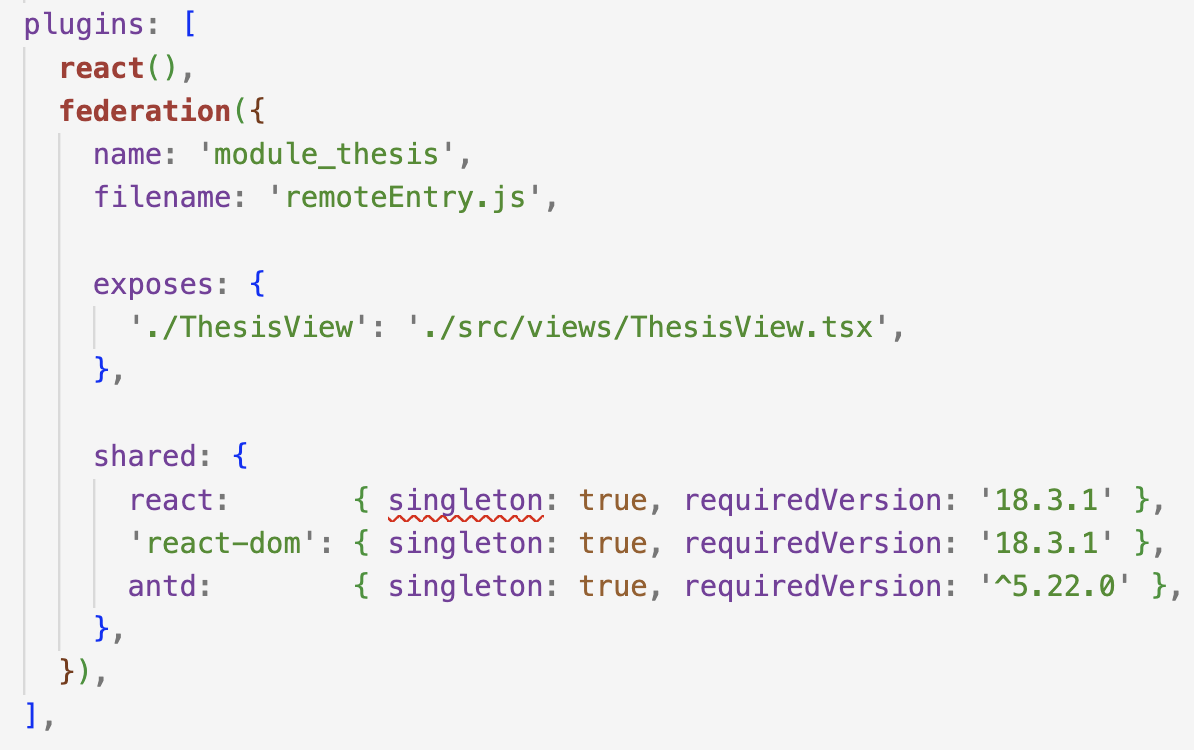
\includegraphics[width=14cm]{images/fig_vite_federation_config.png}
    \caption{Зураг 4.1. \texttt{module-thesis}-ийн \texttt{vite.config.ts} тохиргооны бүтэц. \texttt{name}, \texttt{filename}, \texttt{exposes}, \texttt{shared} дөрвөн гол тохиргооны цэгийг харуулна.}
    \label{fig:vite_config}
\end{figure}

Тохиргооны дөрвөн тулгуур параметрийг тайлбарлая:

\textbf{\texttt{name: 'module\_thesis'}:} Federation-ийн глобал нэрийн
орон зай (namespace). Browser-ийн \texttt{window} объект дээр энэ нэрийн
дор модулийн бүртгэл хийгдэнэ. Нэрийн зөрчлөөс зайлсхийхийн тулд
дор хаяж нэг давхарга нэртэй prefix ашиглах зарчмыг дагав.

\textbf{\texttt{filename: 'remoteEntry.js'}:} Remote MFE-ийн ``агуулгын
хүснэгт'' болох файлын нэр. Host нь энэ URL-г динамикаар \texttt{<script>}
tag хэлбэрт DOM-д оруулах замаар Remote-ийн бүртгэлийг ачаалдаг.

\textbf{\texttt{exposes: \{ './ThesisView': '...' \}}:} Энэ Remote-аас
Host-д нээлттэй байх бүрэлдэхүүнүүд. Дан \texttt{'./ThesisView'} экспортлосон
нь нэгдсэн зарчмыг баримтлж байна~--- нэг Remote нь нэг бизнесийн чадвар.

\textbf{\texttt{shared: \{ react, 'react-dom', antd \}}:} Singleton
хэлбэрт хуваалцагдах хамаарлууд. \texttt{singleton: true} тохиргоо нь
Host болон бүх Remote нэг React instance ашиглахыг баталгаажуулна~---
ингэснээр \texttt{useState}, \texttt{useContext} hook-ууд хөндлөн модулийн
хооронд зөв ажиллана.

\subsection{Runtime Integration: JSF-ийн Script Injection Механизм}

JSF хостын хуудсанд React MFE-г ачаалах гол механизм нь динамик
\texttt{<script>} tag injection юм. Production орчинд Tomcat~8080-д
\texttt{/microfrontends/} замаар static файлуудыг хүргэдэг бол
development орчинд \texttt{http://localhost:30XX} хаягаар Vite-ийн
dev server ажилладаг.

JSF-ийн \texttt{.xhtml} хуудсанд MFE-г ачаалах хэсэг нь дараах
ерөнхий бүтэцтэй:

\begin{figure}[H]
    \centering
    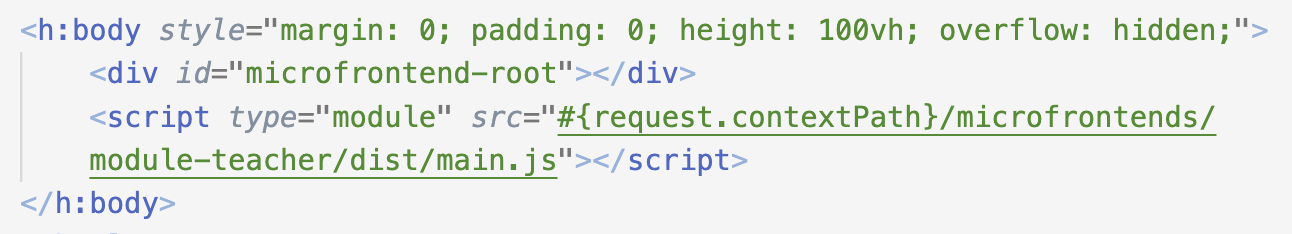
\includegraphics[width=14cm]{images/fig_jsf_script_injection.png}
    \caption{JSF \texttt{.xhtml} хуудасны MFE injection механизм. \texttt{remoteEntry.js} ачаалагдсаны дараа bootstrap.js нь \texttt{<div id="microfrontend-root">} дотор React компонентийг render хийнэ}
    \label{fig:jsf_injection}
\end{figure}

Injection-ийн техникийн дэс дараа:

\begin{enumerate}
  \item JSF Facelets нь хуудсыг server-side render хийхдээ
    \texttt{<div id="microfrontend-root"/>} DOM цэгийг байрлуулна.
  \item \texttt{<script type="module" src=".../remoteEntry.js"/>} tag
    нь браузерт Remote Federation-ийн manifest-ийг ачаална.
  \item \texttt{<script type="module">} блок нь динамик \texttt{import()}
    ашиглан Remote-ийн экспортлосон компонентийг авна.
  \item React-ийн \texttt{createRoot(\#microfrontend-root).render(\ldots)}
    нь тухайн DOM цэгт компонентийг mount хийнэ.
  \item React Router-ийн \textbf{HashRouter} ашигладгийн шалтгаан нь
    JSF-ийн FacesServlet нь \texttt{/student/*} гэх URL pattern-ийг
    хариуцдаг бөгөөд React SPA маршрутлалт нь JSF-тэй зөрчилддгийг
    арилгахын тулд \texttt{/\#/student/dashboard} хэлбэрийн hash-based
    routing хэрэглэнэ.
\end{enumerate}

\subsection{Маршрутлалтын Хүндрэл ба HashRouter Шийдэл}

MFE архитектурт маршрутлалтын хоёр давхарга байдаг: нэгдүгээр давхарга
нь JSF хостын маршрутлалт (\texttt{FacesServlet}-ийн URL pattern), хоёрдугаар
давхарга нь тухайн MFE-ийн React Router дотоод маршрутлалт. Эдгээр хоёр
давхарга зөрчилдөхөд \textbf{``404 Not Found''} буюу JSF-ийн хуудас олдохгүй
алдаа гардаг.

Энэ зөрчлийг шийдвэрлэх хоёр арга байна:

\begin{enumerate}
  \item \textbf{HistoryRouter + Server Catch-all:} Tomcat-д
    \texttt{<url-pattern>/student/*</url-pattern>} бүгдийг нэг JSF
    хуудас руу шилжүүлж, React Router-ийн \texttt{createBrowserRouter}
    ашиглана. Тохиргоо нарийн боловч хэрэглэгчийн URL чухал.
  \item \textbf{HashRouter:} URL-ийн \texttt{\#} хэсэг нь сервер рүү
    хэзээ ч явдаггүй тул JSF-тэй зөрчилддөггүй. React Router-ийн
    \texttt{HashRouter} нь \texttt{/\#/thesis/list} хэлбэрийн URL
    ашиглан дотоод маршрутлалтыг зохицуулна.
\end{enumerate}

Энэ системд \texttt{HashRouter} сонгосны шалтгаан нь: JSF-ийн \texttt{web.xml}
болон \texttt{faces-config.xml}-ийн нарийн URL pattern тохиргоог өөрчлөх
нь монолитийн дотоод урсгалд нөлөөлнө гэсэн эрсдэлтэй байсан тул
хамгийн бага өөрчлөлтийн зарчмаар \texttt{HashRouter}-ийг сонгов.

\subsection{JWT болон Глобал Төлөвийн Хуваалцалт}

JSF хост болон React MFE хоорондын хэрэглэгчийн нэвтрэлтийн мэдлэгийн
хуваалцалт нь архитектурын хамгийн нарийн хэсэг юм. Хэрэглэгч
\texttt{module-auth}-д нэвтрэхэд дараах дараалал гүйцэтгэгдэнэ:

\begin{figure}[H]
    \centering
    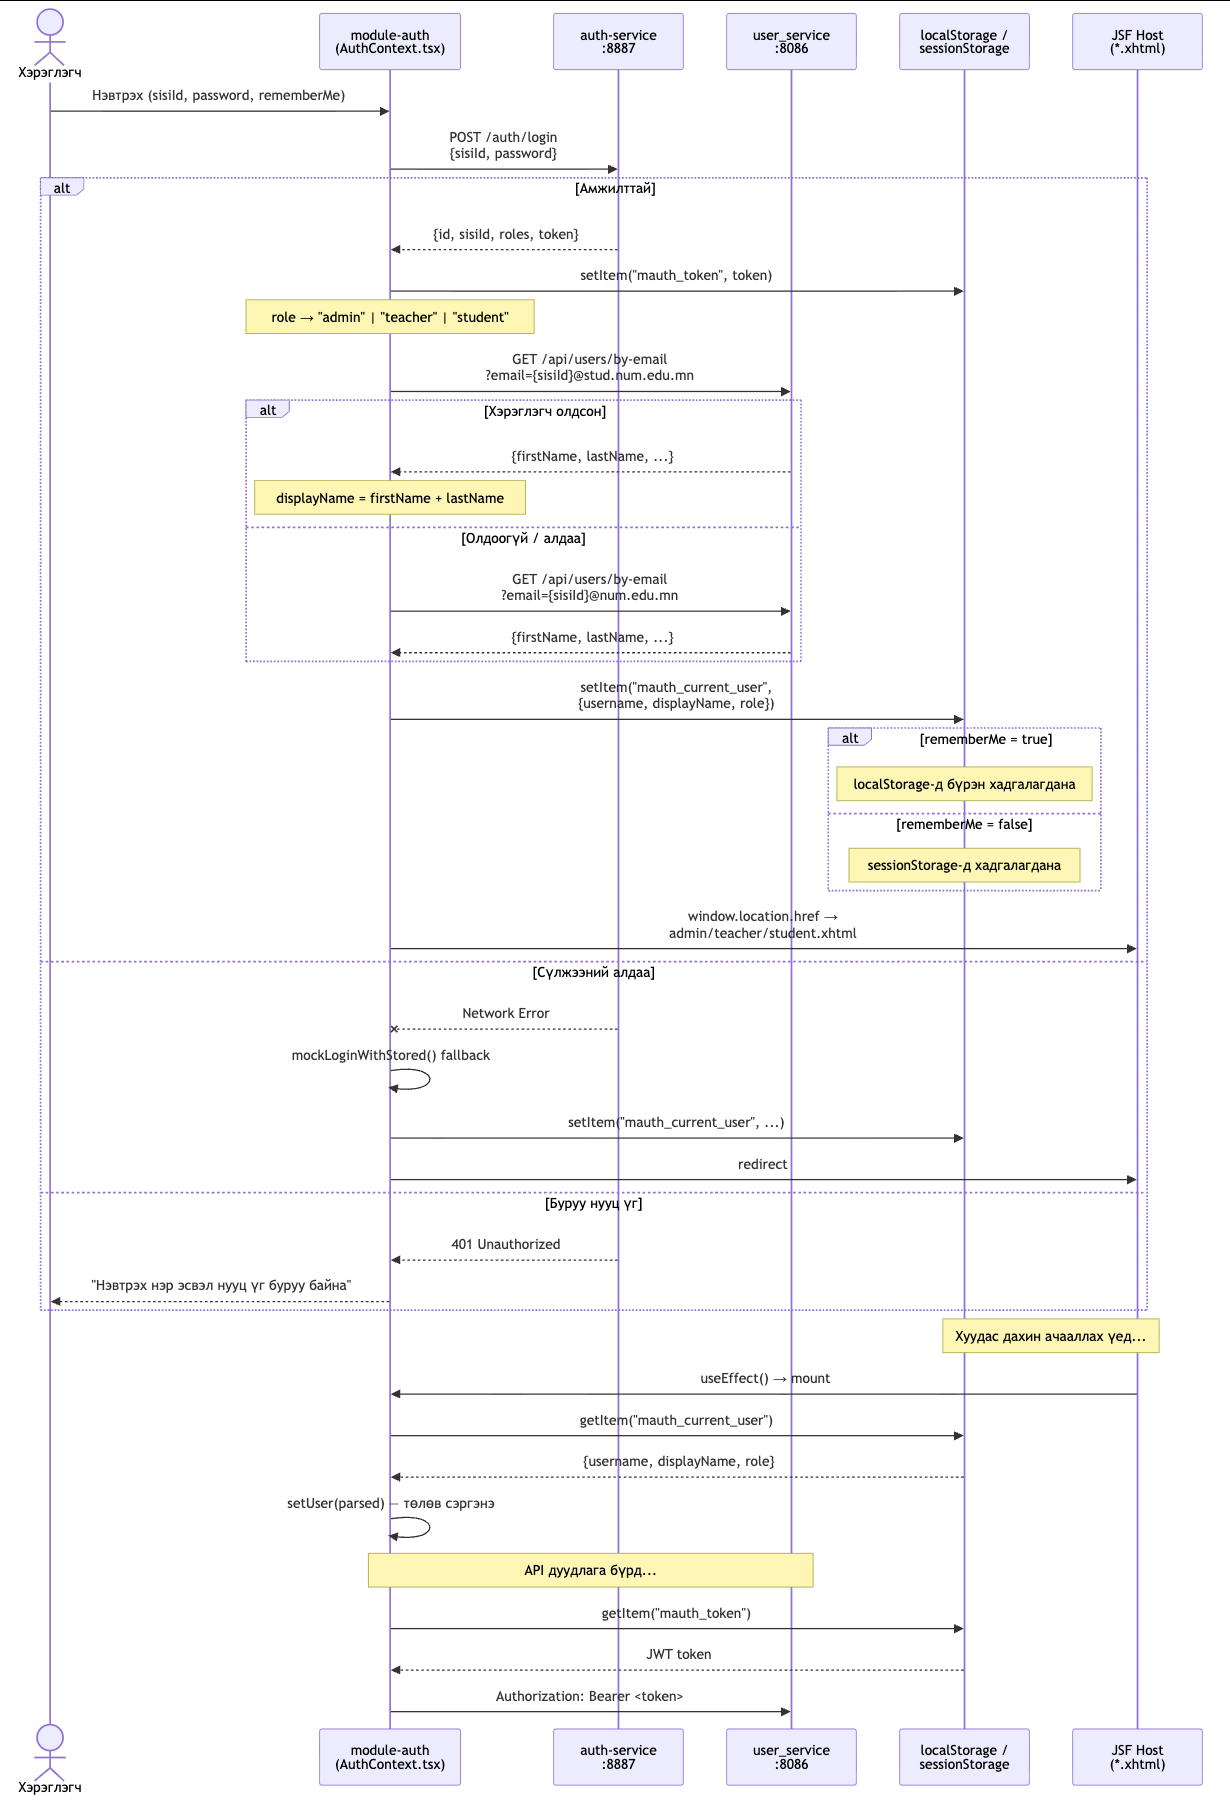
\includegraphics[width=14cm]{images/fig_jwt_flow_sequence.png}
    \caption{JWT нэвтрэлтийн дараалалт диаграм. Auth MFE нь токений хүсэлт илгээж, хүлээн авсан JWT-г localStorage-д хадгалах бөгөөд бусад MFE-ууд нь тэндээс JWT-г уншиж API дуудлагад ашиглана}
    \label{fig:jwt_flow}
\end{figure}

Хуваалцах механизм нь \texttt{localStorage} дотор тодорхой key-д JSON
объект хэлбэрт хадгалагдана:

\begin{itemize}
  \item \texttt{mauth\_token}: JWT Bearer токен~--- API дуудлага бүрийн
    \texttt{Authorization: Bearer \ldots} header-т ашиглагдана.
  \item \texttt{mauth\_current\_user}: \texttt{\{username, displayName,
    role\}} бүтэцтэй JSON~--- хэрэглэгчийн нэр, дүр зэргийг хадгалана.
\end{itemize}

Дизайн шийдвэрийн үндэслэл: \texttt{localStorage} нь хуудас дахин
ачааллагдах (page refresh) болон хэд хэдэн browser tab хооронд бүтэн
хадгалагддаг. \texttt{sessionStorage} нь tab хаагдахад устдаг тул
``Намайг санах'' (Remember Me) функцийг дэмжихгүй. Аюулгүй байдлын
хувьд \texttt{HttpOnly Cookie} нь XSS халдлагаас хамгаалалт сайн боловч
JSF-ийн хуудасны дагуу cookie scope нарийн удирдлага шаардана~---
тул энэ прототипд \texttt{localStorage} ашигласан бөгөөд үйлдвэрлэлийн
орчинд \texttt{HttpOnly} cookie руу шилжихийг зөвлөмж болгоно.

\texttt{AuthContext.tsx} нь React-ийн Context API-д суурилсан global
state provider бөгөөд MFE модуль бүрийн root-д байрладаг. Хуудас
ачааллагдах бүрт localStorage-ийн утгыг уншиж, хэрэглэгчийн төлөвийг
сэргээдэг. Нэвтрэлтийн дараалал нь дараах байна: эхлээд
\texttt{POST http://localhost:8887/auth/login} руу \texttt{\{sisiId,
password\}} илгээнэ; амжилттай тохиолдолд хариуд JWT токен болон
дүрийн мэдээлэл ирнэ; дараа нь \texttt{GET http://localhost:8086/api/users/by-email}
руу хүсэлт илгээж хэрэглэгчийн дэлгэрэнгүй нэрийг авна; эцэст нь
дүрд тохирсон URL руу чиглүүлнэ.

\subsection{Shared-UI ба Singleton Хамаарлын Зохицуулалт}

3-р бүлэгт тодорхойлсон \texttt{shared-ui} модуль нь практик хэрэгжүүлэлтэд
нарийн техникийн хүндрэлтэй тулгарав. Анх nested federation загвараар~---
\texttt{module-thesis} нь \texttt{shared\_ui} Remote-ийг агуулах~---
загварчилсан боловч хэрэгжүүлэлтийн явцад критик алдаа илэрлээ:

\texttt{TypeError: Failed to resolve module specifier '\$\{\_\_federation\_expose\_./SharedUI\}'}

Энэ алдааны үндэс нь \texttt{@originjs/vite-plugin-federation} нь
Remote-ийн \texttt{remoteEntry.js}-д Remote-ийн Remote-ийн URL template-ийг
динамикаар тохируулах механизм дутмаг байдаг явдал юм. Tomcat-д статик
файл хэлбэрт хүргэгдсэн Remote нь өөрийн nested Remote-ийн URL-г
тодорхойлж чадахгүй.

\textbf{Шийдэл:} Nested federation-ийн оронд \texttt{shared-ui}-ийн
бүрэлдэхүүнүүдийг (\texttt{PageHeader}, \texttt{PortalTabs},
\texttt{StatusBadge}, \texttt{DataTable}) тухайн Remote-ийн дотор шууд
нэгтгэж, Ant Design-ийг federation-ийн \texttt{shared singleton}
механизмаар хуваалцана. Энэ нь кодын хуулбарлалтын зардалтай боловч
runtime-д нэг antd instance ашиглагддаг тул bundle хэмжээ нэмэгдэхгүй.

\begin{figure}[H]
    \centering
    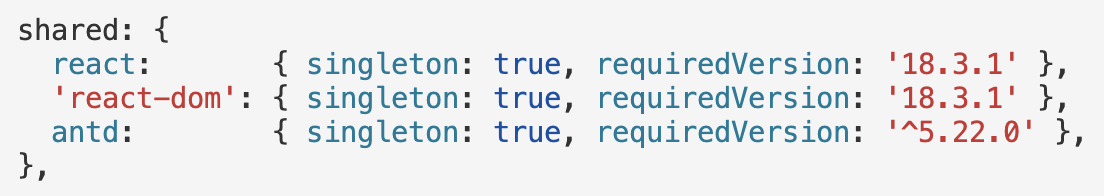
\includegraphics[width=14cm]{images/fig_shared_singleton_pattern.png}
    \caption{Shared Singleton загварын зохицуулалт. Antd нь нэгдсэн singleton хэлбэрт ачааллагдаж, Remote модуль бүр энэ нэг instance-ийг ашиглана~--- nested federation-ийн алдааг арилгана. Эх сурвалж: зохиогчийн судалгаа, 2026.}
    \label{fig:shared_singleton}
\end{figure}

\subsection{Build ба Deploy Паплайн}

Хэрэгжүүлэлтийн орчинд \texttt{build-modules.sh} shell скрипт нь
бүх MFE модулийг дараалан build хийж, \texttt{dist/} гаралтыг
Tomcat-ийн \texttt{webapps/microfrontends/\{module-name\}/dist/}
хавтаст хуулдаг. Скриптийн ерөнхий урсгал нь:

\begin{enumerate}
  \item MFE модуль бүрийн \texttt{npm run build} ажиллуулна.
  \item \texttt{dist/assets/remoteEntry.js} файлыг \texttt{dist/}
    root рүү хуулна~--- \texttt{@originjs}-ийн хуучин хувилбар нь
    \texttt{remoteEntry.js}-г \texttt{dist/assets/} дотор үүсгэдэг
    тул Host-ийн URL тохиргоотой зөрчилддгийг засна.
  \item Томкат нь \texttt{/microfrontends/\{module\}/dist/remoteEntry.js}
    замаар тухайн Remote-ийн manifest-ийг хүргэнэ.
\end{enumerate}

\begin{figure}[H]
    \centering
    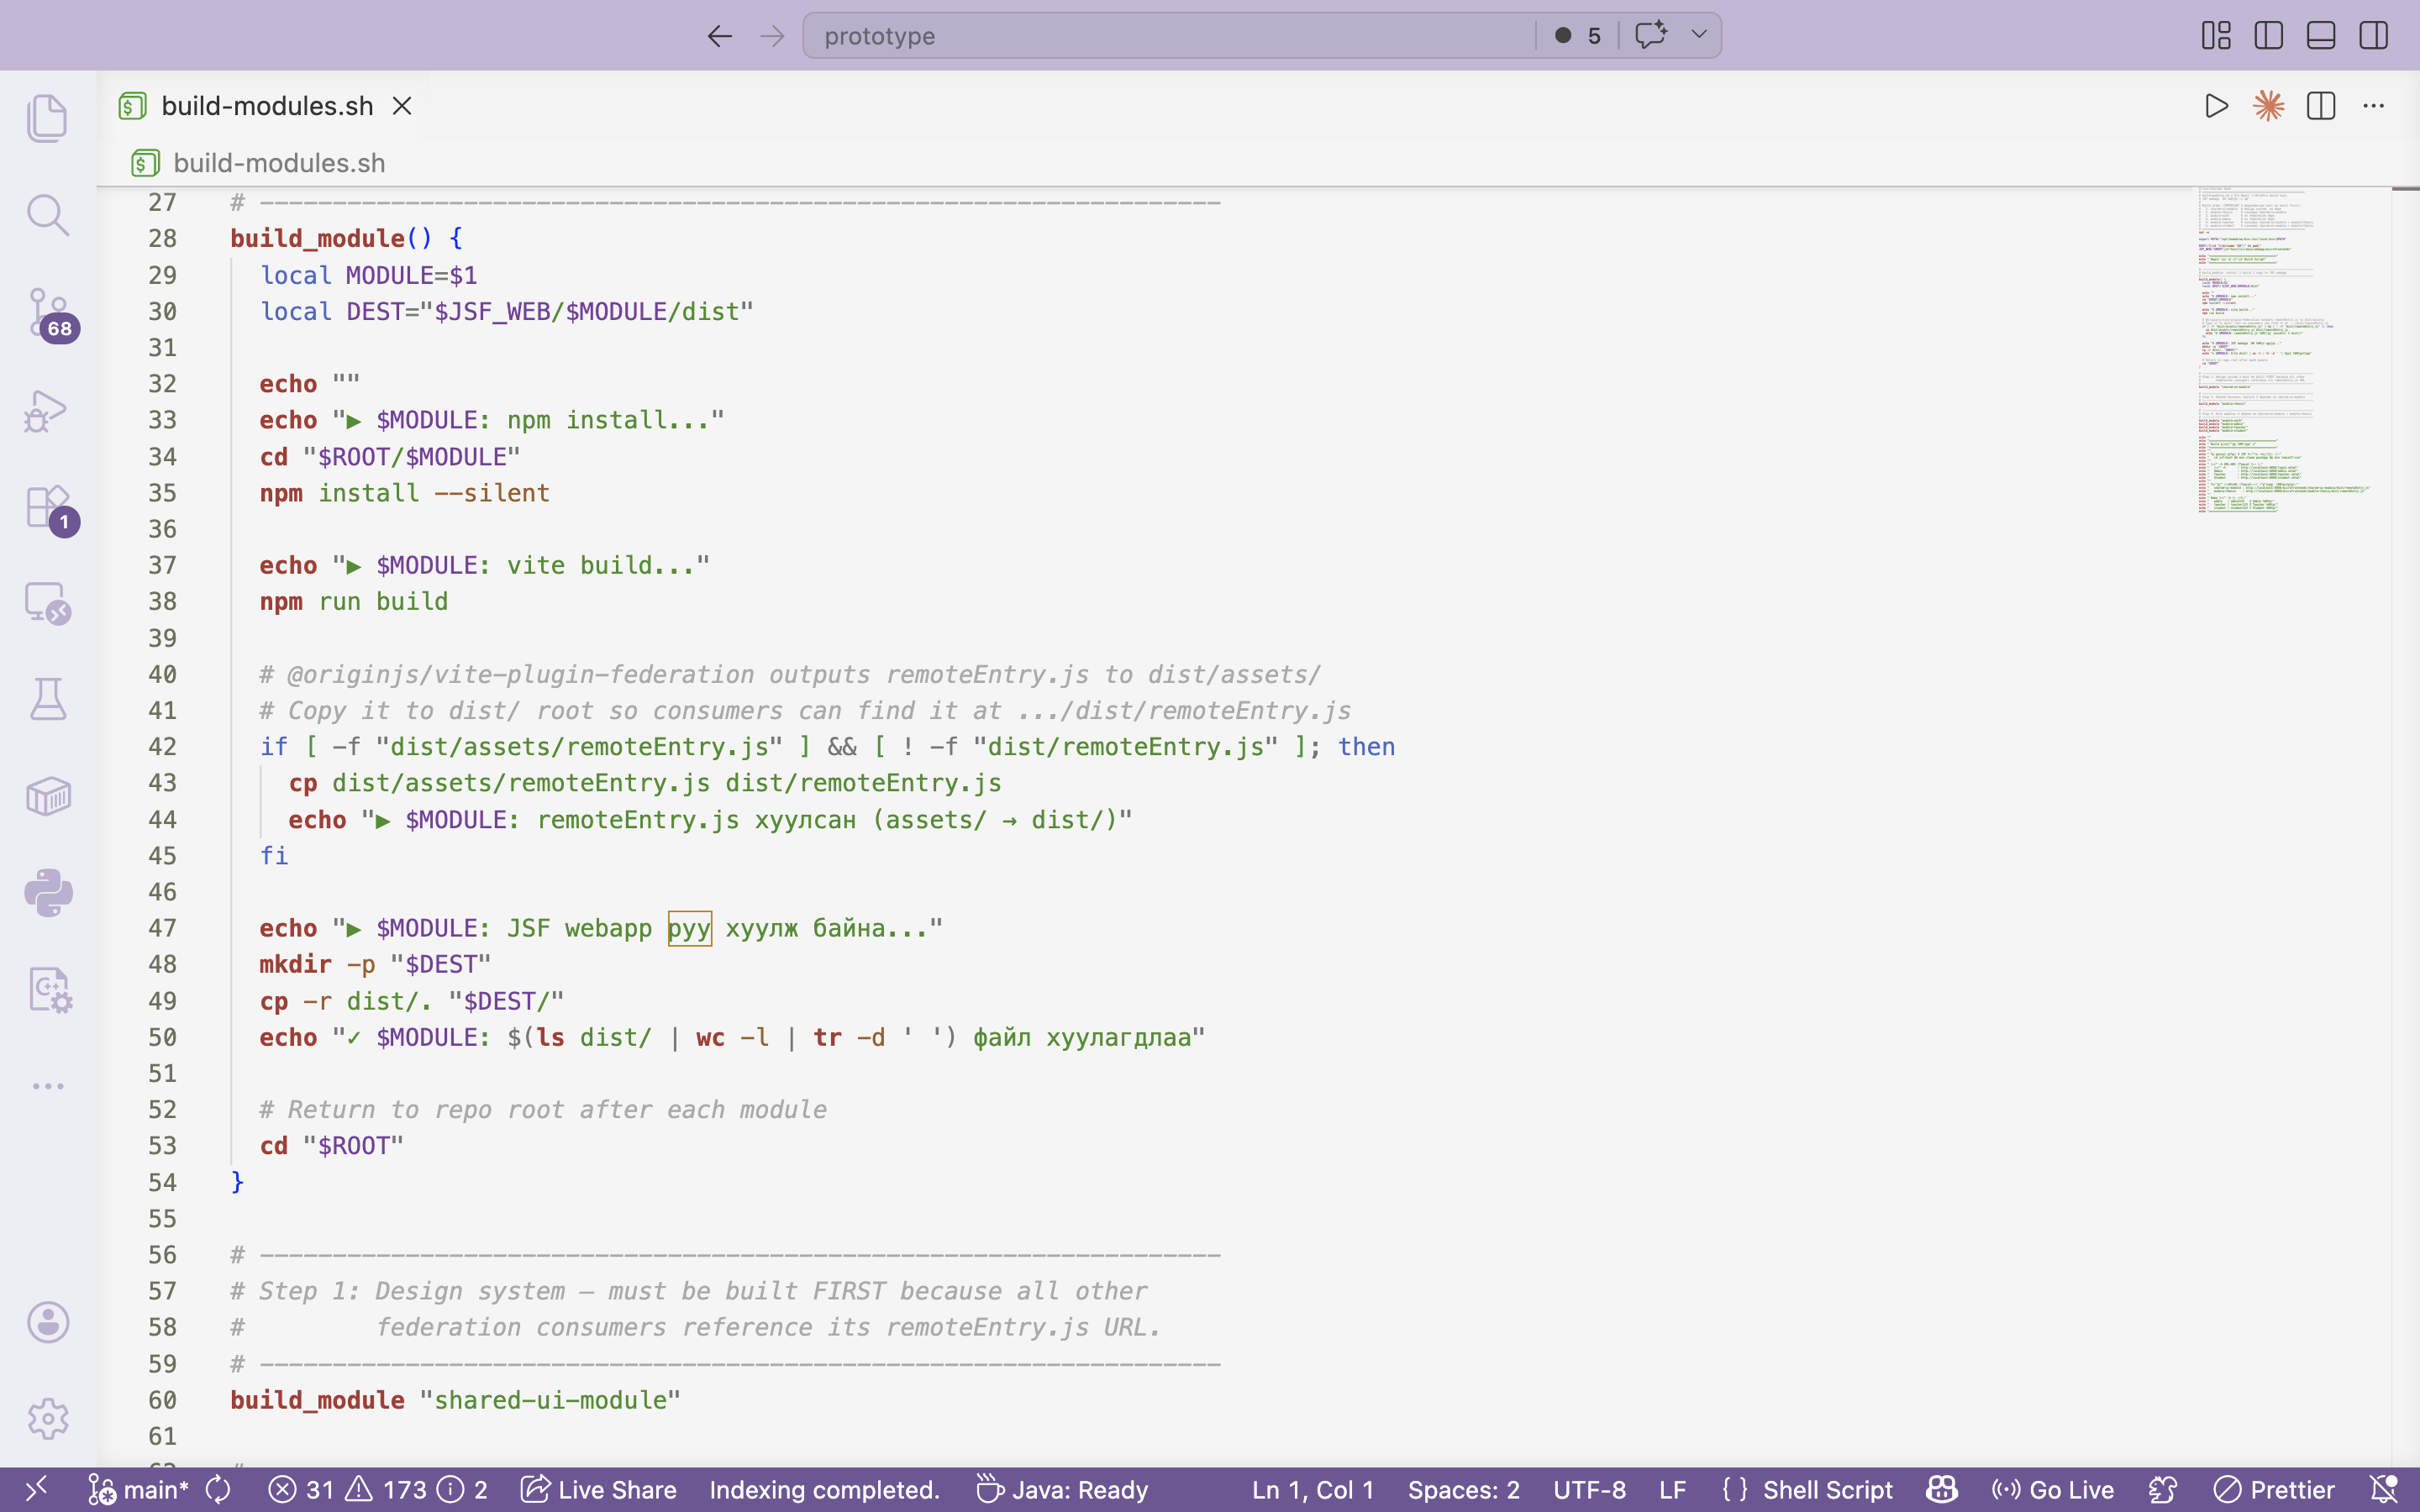
\includegraphics[width=14cm]{images/fig_build_deploy_pipeline.png}
    \caption{Зураг 4.5. Build ба Deploy паплайны урсгалын диаграм. Модуль тус бүрийн Vite build гаралт нь Tomcat-ийн webapps хавтасрт хуулагдаж, нэгдсэн байдлаар 8080 порт дээр хүргэгдэнэ. Эх сурвалж: зохиогчийн судалгаа, 2026.}
    \label{fig:build_pipeline}
\end{figure}

% ─────────────────────────────────────────────────────────────────────
\section{Backend Хэрэгжүүлэлт}
% ─────────────────────────────────────────────────────────────────────

\subsection{Spring Boot болон Spring WebFlux-ийн Сонголт}

Backend микросервисүүдийн хэрэгжүүлэлтэд Java~21 болон Spring Boot~3.2.x
framework-ийг ашиглав. Гэвч 3-р бүлгийн 3.3.2-т тодорхойлсон масштабдах
чадварын шаардлагын дагуу уламжлалт \textbf{Spring MVC} (thread-per-request)
загварын оронд \textbf{Spring WebFlux} (reactive, event-loop) загварыг
сонгов.

Spring MVC нь request бүрт нэг thread хуваарилдаг тул 1,000 зэрэгцэх
хүсэлт нь 1,000 thread шаарддаг~--- JVM-ийн thread stack дундажаар 512~КБ
тул 1,000 thread нь $\approx$~500~МБ санах ой хэрэглэнэ. Spring WebFlux
нь Netty-ийн Non-blocking I/O event-loop дээр суурилж, CPU-ийн цөмийн
тоо ($n$) thread-аар хэдэн мянган зэрэгцэх холболтыг удирддаг.

\textbf{Hexagonal Architecture (Ports and Adapters):} Сервис тус бүрийн
дотоод бүтэц нь Alistair Cockburn (2005)-ийн Hexagonal Architecture
зарчмаар зохион байгуулагдсан:

\begin{itemize}
  \item \textbf{Domain Layer:} Бизнесийн логик агуулсан цөм~---
    жишээ нь \texttt{Thesis}, \texttt{WorkflowState} домейн объектууд.
    Аль ч фреймворкоос тусгаарлагдсан цэвэр Java/Kotlin класс.
  \item \textbf{Application Layer (Ports):} Use Case интерфэйс~---
    \texttt{CreateStudentUseCase}, \texttt{FindUserUseCase},
    \texttt{SubmitThesisUseCase}. Домейн логикийг хэрхэн дуудах
    гэрээг тодорхойлно.
  \item \textbf{Adapter Layer:} Гадаад ертөнцтэй холбогч~---
    \texttt{UserController} (HTTP adapter), \texttt{UserR2dbcRepository}
    (persistence adapter), \texttt{NotificationWebSocketAdapter}
    (messaging adapter).
\end{itemize}

\begin{figure}[H]
    \centering
    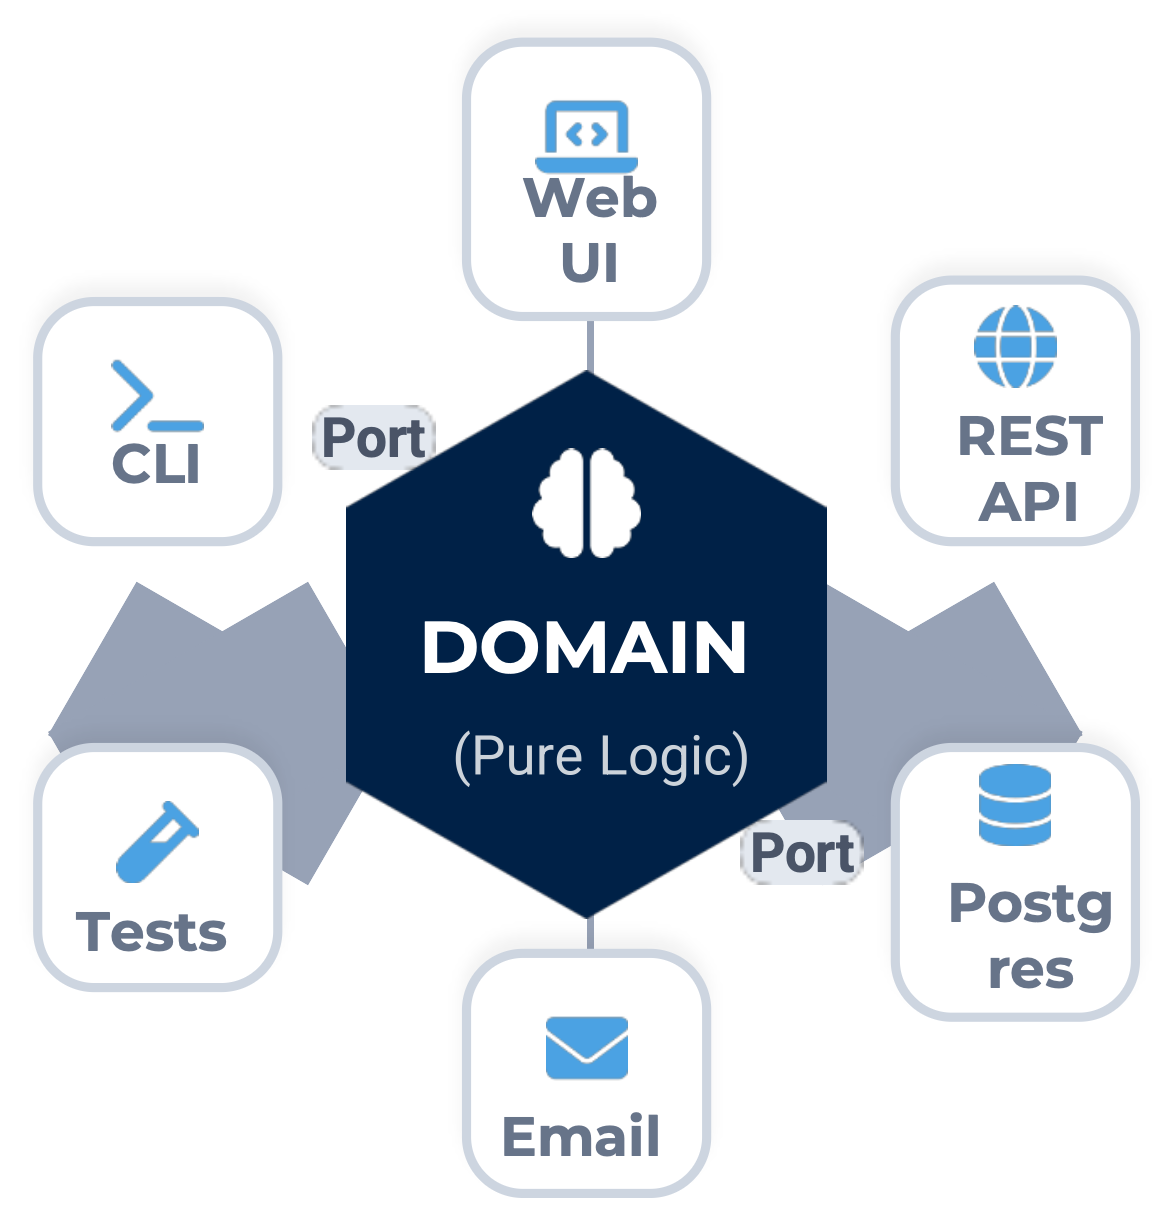
\includegraphics[width=14cm]{images/fig_hexagonal_architecture.png}
    \caption{Hexagonal Architecture-ийн \texttt{user\_service} дахь хэрэгжүүлэлтийн бүтэц. Домейн давхарга нь дотор цагирагт, Port-ууд нь дунд цагирагт, Adapter-ууд нь гадаад цагирагт байрлана. Эх сурвалж: зохиогчийн судалгаа, 2026.}
    \label{fig:hexagonal_arch}
\end{figure}

\subsection{Микросервис Тус Бүрийн Хэрэгжүүлэлтийн Нарийн}

\subsubsection{auth-service ба JWT Токений Хэрэгжүүлэлт}

\texttt{auth-service} нь \texttt{sisiId} болон нууц үг хүлээн авч, хэрэглэгчийн
бичлэгтэй харьцуулж, \texttt{jjwt}~(Java JWT) санг ашиглан токен
үүсгэнэ. Токений payload нь \texttt{\{sub: sisiId, roles: [...],
iat: epochSeconds, exp: iat+86400\}} бүтэцтэй. Нийтийн болон хувийн
түлхүүрийн хос (RSA-256)-ийн оронд энэ прототипд HMAC-SHA256 алгоритмтай
нийтлэг нууц key ашиглагдав~--- үйлдвэрлэлийн орчинд RSA key pair
болон Key Management Service (KMS) ашиглахыг зөвлөмж болгоно.

\texttt{authorization-service} нь дүр болон эрхийн матрицийг удирдана.
\texttt{ROLE\_ADMIN}, \texttt{ROLE\_TEACHER}, \texttt{ROLE\_STUDENT},
\texttt{ROLE\_COMMITTEE\_MEMBER} дүрүүд тодорхойлогдсон бөгөөд endpoint
бүр дээр Spring Security-ийн \texttt{@PreAuthorize} annotationоор
хандах эрхийн шалгалт хэрэгжинэ.

\subsubsection{user\_service-ийн Reactive Хэрэгжүүлэлт}

\texttt{user\_service} нь Spring WebFlux болон R2DBC-г хослуулан ашиглах
бөгөөд \texttt{UserController}-д хэрэглэгчийн CRUD болон хайлтын
endpoint-ууд хэрэгждэнэ. \texttt{/api/users/by-email} endpoint нь
\texttt{UserR2dbcRepository.findByEmail(String email)} reactive метод
дуудаж, \texttt{Mono<User>} буцаана~--- энэ нь AuthContext-ийн
display name lookup-д зориулан нэмэгдсэн.

\texttt{UserR2dbcRepository} нь \texttt{ReactiveCrudRepository<User, String>}
интерфэйсийг өргөтгөсөн бөгөөд Spring Data R2DBC нь SQL query-г
\texttt{findBy\{FieldName\}} нэрлэлтийн конвенцоос автоматаар үүсгэнэ.
Энэ нь ``конвенц дагасан тохиргоо'' (convention over configuration)
зарчмын практик хэрэглэлт бөгөөд boilerplate кодын хэмжээг мэдэгдэхүйц
бууруулна.

\subsubsection{workflow\_service-ийн State Machine Хэрэгжүүлэлт}

\texttt{workflow\_service} нь дипломын ажлын статус шилжилтийг хариуцна.
State Machine нь Java-ийн enum болон явцын хамгаалагдсан шилжилтийн
матрицаар хэрэгжинэ:

\begin{table}[H]
    \centering
    \caption{Дипломын ажлын статус шилжилтийн зөвшөөрөгдсөн матриц}
    \label{tab:workflow_transitions}
    \renewcommand{\arraystretch}{0.7}
    \begin{tabular}{lll}
        \toprule
        \textbf{Одоогийн статус} & \textbf{Зорилтот статус} & \textbf{Хэн гүйцэтгэх} \\
        \midrule
        DRAFT              & SUBMITTED           & Оюутан \\
        SUBMITTED          & UNDER\_REVIEW       & Удирдагч багш \\
        SUBMITTED          & REJECTED            & Удирдагч багш \\
        UNDER\_REVIEW      & REVISION\_REQUESTED & Удирдагч багш \\
        UNDER\_REVIEW      & APPROVED            & Удирдагч багш \\
        REVISION\_REQUESTED & SUBMITTED          & Оюутан \\
        APPROVED           & DEFENSE\_SCHEDULED  & Систем / Админ \\
        DEFENSE\_SCHEDULED & DEFENDED            & Хорооны гишүүн \\
        DEFENDED           & ARCHIVED            & Систем \\
        \bottomrule
    \end{tabular}
\end{table}

Зөвшөөрөгдөөгүй шилжилтийн оролдлого нь \texttt{HTTP 422 Unprocessable
Entity} буцаах бөгөөд хариу body нь шилжилт яагаад зөвшөөрөгдөхгүй
байгаа шалтгааны тайлбарыг агуулна.

\subsection{API Gateway-ийн Тохиргоо}

Тус системд тусдаа API Gateway сервис биш харин \textbf{Tomcat-ийн
reverse proxy} тохиргоо gateway-ийн үүрэг гүйцэтгэнэ. Apache Tomcat
нь \texttt{server.xml}-д \texttt{ProxyPass} директивоор (эсвэл Nginx
reverse proxy хослуулан) backend сервисүүд рүү HTTP хүсэлтийг
чиглүүлнэ. Энэ нь Nginx эсвэл Spring Cloud Gateway-тай харьцуулахад
хялбар боловч илүү нарийн CORS, rate limiting, circuit breaker
хяналт шаарддаг тул ирээдүйн шатанд тусдаа gateway нэвтрүүлэх
хэрэгцээ байна.

Frontend JavaScript-аас API дуудлагын CORS тохиргоо нь сервис
бүрийн \texttt{application.yml}-д тохируулагдсан:

\begin{figure}[H]
    \centering
    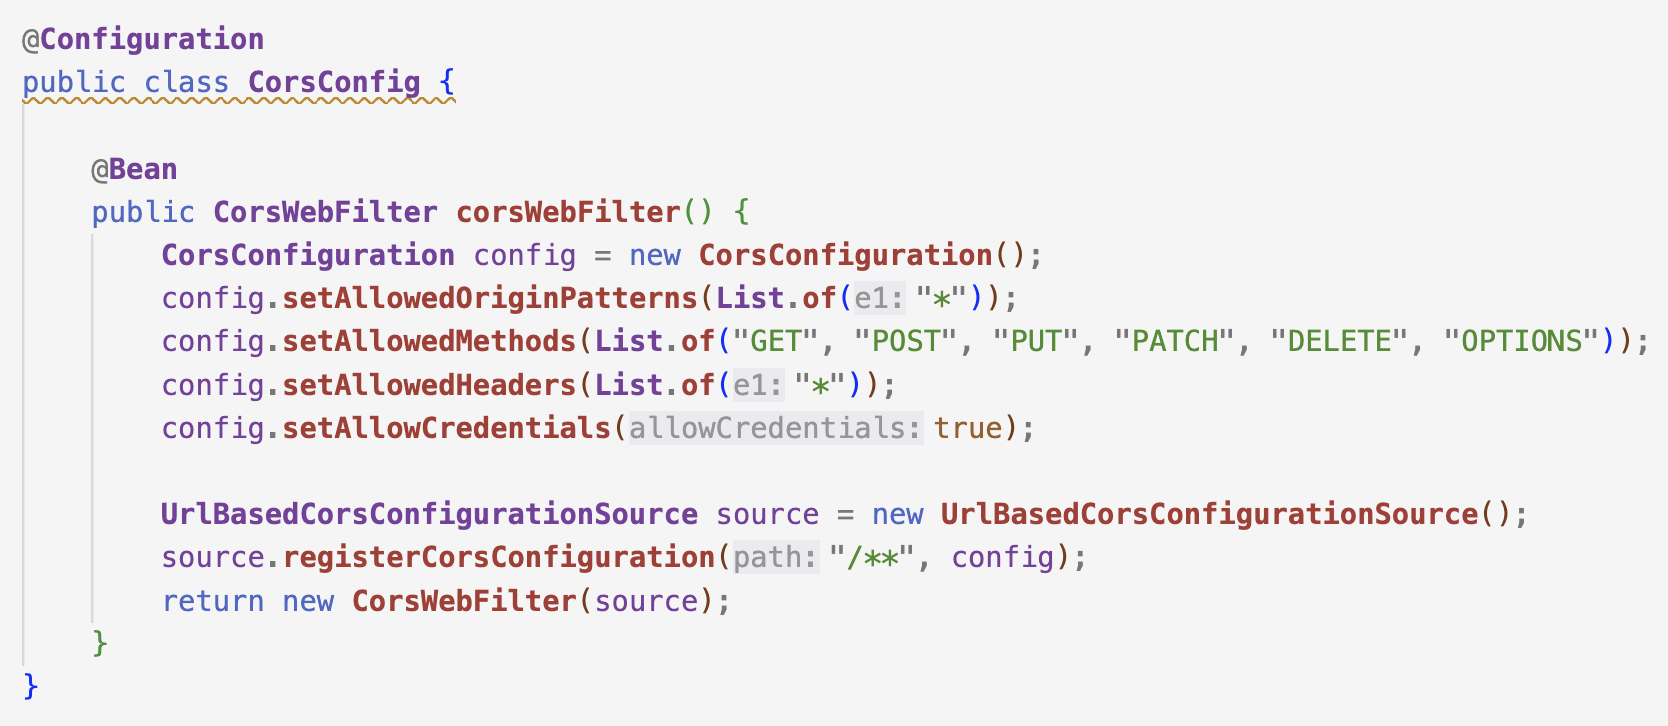
\includegraphics[width=14cm]{images/fig_cors_config.png}
    \caption{Зураг 4.7. Spring WebFlux-ийн CORS тохиргооны жишээ. \texttt{allowedOrigins} нь Tomcat-ийн 8080 порт, \texttt{allowedMethods} нь REST стандартын бүх method-уудыг агуулна. Эх сурвалж: зохиогчийн судалгаа, 2026.}
    \label{fig:cors_config}
\end{figure}

\texttt{allowedOrigins: "http://localhost:8080"} нь зөвхөн JSF хостын
хаягаас ирсэн AJAX хүсэлтийг зөвшөөрнө. Үйлдвэрлэлийн орчинд
энэ нь бодит domain нэрийг агуулна, wildcard (\texttt{*}) ашиглахаас
зайлсхийнэ.

\subsection{Distributed Tracing-ийн Хэрэгжүүлэлт}

Сервисүүдийн хоорондох хүсэлтийн урсгалыг хянах Distributed Tracing-ийг
OpenTelemetry Java Agent болон Jaeger-ийн хослолоор хэрэгжүүлэв.
JVM startup parameter-т \texttt{-javaagent:opentelemetry-agent.jar}
нэмснээр application кодыг өөрчлөхгүйгээр HTTP request бүрт
\texttt{traceparent}, \texttt{tracestate} W3C стандартын trace header
автоматаар нэмэгдэнэ.

Нэг хэрэглэгчийн хүсэлт хэд хэдэн сервисийг дамжих бүрт нэг
\texttt{traceId}-ийн дор бүх span-ууд нэгтгэгдэнэ~--- Jaeger UI-д
waterfall диаграм хэлбэрт харагддаг бөгөөд сервис бүрийн саатал
(latency contribution) тус тусад нь хэмжигдэнэ. Оюутан дипломын ажил
илгээхэд \texttt{POST /api/thesis/submit}-ийн trace нь
\texttt{auth-service} (JWT шалгах), \texttt{thesis-service}
(бичлэг шинэчлэх), \texttt{workflow-service} (статус шилжүүлэх),
\texttt{notification-service} (мэдэгдэл илгээх) гэсэн 4 span агуулдаг.

% ─────────────────────────────────────────────────────────────────────
\section{Өгөгдлийн Сангийн Хэрэгжүүлэлт}
% ─────────────────────────────────────────────────────────────────────

\subsection{PostgreSQL болон R2DBC-ийн Сонголт}

3-р бүлгийн өгөгдлийн давхаргын загварчлалд PostgreSQL-г харилцааны
(relational) өгөгдлийн санаар, R2DBC-г реактив driver хэлбэрт сонгосон
байсан. Практик хэрэгжүүлэлтэд PostgreSQL~16.2 болон
\texttt{io.r2dbc:r2dbc-postgresql:1.0.4} driver ашиглав.

\textbf{Яагаад PostgreSQL:} Дипломын ажлын бизнесийн логик нь олон
харилцаатай өгөгдлийн бүтэц (User $\leftrightarrow$ Thesis
$\leftrightarrow$ Committee $\leftrightarrow$ Evaluation) агуулдаг
тул харилцааны бүрэн бүтэн байдлын баталгаа (referential integrity),
ACID transaction, SQL-ийн хүчирхэг query боломж шаардагдана. Document
store (MongoDB) нь schema-flexible боловч JOIN-ийн хэрэгцээтэй энэ
домейнд неудобен.

\textbf{Яагаад R2DBC (JDBC биш):} Spring WebFlux-ийн event-loop
загвар нь blocking JDBC дуудлагатай ``reactive pollution'' (цуваа
блоклолт) асуудалд орно~--- blocking call нь event-loop thread-ийг
хааж, бусад хүсэлтийн хариулт удаашралд орно. R2DBC нь Non-blocking
reactive driver тул WebFlux-тэй зохистой хэрэгждэнэ.

\subsection{Schema Тодорхойлолт ба Migration}

Сервис тус бүрийн өгөгдлийн сангийн schema нь тухайн сервисийн
\texttt{src/main/resources/schema\_\{service\_name\}.sql} файлд
тодорхойлогдсон. Эхний нэвтрэлтэд Spring Boot-ийн
\texttt{spring.sql.init.mode: always} тохиргоог ашиглан schema
автоматаар үүснэ. Үйлдвэрлэлийн орчинд Flyway эсвэл Liquibase
migration хэрэгслийг ашиглахыг зөвлөмж болгоно.

\texttt{user\_service}-ийн \texttt{schema\_user\_service.sql}-ийн
гол хэсгийг жишээ болгон дурдвал:

\begin{lstlisting}[language=sql, caption={\texttt{user\_service}-ийн SQL schema-ийн жишээ. \texttt{users}, \texttt{departments} хүснэгтүүдийн DDL болон constraint-уудыг харуулна.}, label={lst:schema_sql}]
CREATE TABLE IF NOT EXISTS users (
    id              VARCHAR(255) PRIMARY KEY,
    first_name      VARCHAR(255) NOT NULL,
    last_name       VARCHAR(255) NOT NULL,
    email           VARCHAR(255) NOT NULL UNIQUE,
    department_id   VARCHAR(255),
    system_role     VARCHAR(50)  NOT NULL,
    active          BOOLEAN      NOT NULL DEFAULT TRUE,
    photo_url       VARCHAR(1000),
    created_at      TIMESTAMP    NOT NULL DEFAULT CURRENT_TIMESTAMP,
    CONSTRAINT chk_system_role
        CHECK (system_role IN ('ADMIN','STUDENT','TEACHER','DEPARTMENT_HEAD'))
);

CREATE TABLE IF NOT EXISTS students (
    id                  VARCHAR(255) PRIMARY KEY,
    user_id             VARCHAR(255) NOT NULL UNIQUE
        REFERENCES users(id) ON DELETE CASCADE,
    student_id          VARCHAR(255) NOT NULL UNIQUE,  
    major               VARCHAR(255),
    has_approved_topic  BOOLEAN NOT NULL DEFAULT FALSE
);

CREATE TABLE IF NOT EXISTS teachers (
    id                          VARCHAR(255) PRIMARY KEY,
    user_id                     VARCHAR(255) NOT NULL UNIQUE
        REFERENCES users(id) ON DELETE CASCADE,
    position                    VARCHAR(255),
    supervisor_quota            INT NOT NULL DEFAULT 5,
    current_supervised_count    INT NOT NULL DEFAULT 0,
    CONSTRAINT chk_quota_positive
        CHECK (supervisor_quota > 0),
    CONSTRAINT chk_count_non_negative
        CHECK (current_supervised_count >= 0)
);

CREATE TABLE IF NOT EXISTS departments (
    id              VARCHAR(255) PRIMARY KEY,
    user_id         VARCHAR(255) NOT NULL UNIQUE
        REFERENCES users(id) ON DELETE CASCADE,
    department_name VARCHAR(255) NOT NULL
);
CREATE INDEX IF NOT EXISTS idx_users_email       ON users(email);
CREATE INDEX IF NOT EXISTS idx_users_role        ON users(system_role);
CREATE INDEX IF NOT EXISTS idx_users_dept        ON users(department_id);
CREATE INDEX IF NOT EXISTS idx_students_user     ON students(user_id);
CREATE INDEX IF NOT EXISTS idx_students_sisi     ON students(student_id);
CREATE INDEX IF NOT EXISTS idx_teachers_user     ON teachers(user_id);
CREATE INDEX IF NOT EXISTS idx_departments_user  ON departments(user_id);

\end{lstlisting}

\texttt{user\_type} нь PostgreSQL-ийн native \texttt{ENUM} гэхийн
оронд \texttt{VARCHAR(20) CHECK (user\_type IN (...))}-ийн хэлбэрт
хэрэгжсэн~--- R2DBC-ийн хуучин хувилбарт native enum-ийн codec
авторегистр хийгддэггүй тул энэ шийдэл нь портатив, хамааралгүй.

\subsection{Connection Pooling ба Гүйцэтгэлийн Тохируулга}

R2DBC нь өөрийн \texttt{r2dbc-pool} connection pool-тай. Сервис
тус бүрийн \texttt{application.yml}-д connection pool-ийн тохиргоо
дараах байдлаар хийгдэв:

\begin{table}[H]
    \centering
    \caption{R2DBC Connection Pool-ийн тохиргооны параметрүүд}
    \label{tab:r2dbc_pool}
    \renewcommand{\arraystretch}{0.7}
    \begin{tabular}{lrl}
        \toprule
        \textbf{Параметр} & \textbf{Утга} & \textbf{Тайлбар} \\
        \midrule
        \texttt{initial-size}       & 5   & Эхлэлийн холболтын тоо \\
        \texttt{max-size}           & 20  & Хамгийн их зэрэгцэх холболт \\
        \texttt{max-idle-time}      & 30м & Идэвхгүй холболтын хамгийн их хугацаа \\
        \texttt{max-life-time}      & 60м & Холболтын нийт амьдах хугацаа \\
        \texttt{acquire-retry}      & 3   & Холболт авах оролдлогын тоо \\
        \texttt{validation-query}   & SELECT~1 & Холболт шалгах query \\
        \bottomrule
    \end{tabular}
\end{table}

\texttt{max-size: 20} нь нэг PostgreSQL-ийн default \texttt{max\_connections}
(100)-тай харьцуулахад таван сервис нэгэн зэрэг ажиллахад нийт
$5 \times 20 = 100$ холболтын хязгаарт ойрхон болно. Үйлдвэрлэлийн
орчинд \texttt{pgBouncer} connection pooler нэмэх нь PostgreSQL-ийн
connection-г дахин ашиглах боломж олгоно.

\subsection{Cross-Service Мэдээллийн Нийцэл}

Практик хэрэгжүүлэлтэд distributed transaction (2PC) ашиглахын оронд
дараах хоёр механизмыг хэрэглэв:

\textbf{Application-level Retry:} \texttt{workflow\_service}-ийн
\texttt{WebClient} нь upstream сервис рүү хүсэлт илгээхдээ
\texttt{retry(3).retryWhen(Retry.backoff(3, Duration.ofMillis(500)))}
оператораар экспоненциал backoff retry хэрэгжүүлнэ. Гурван оролдлогын
дараа амжилтгүй бол \texttt{workflow\_service} нь локал статус шилжилтийг
``rollback'' хийж, хэрэглэгчид алдааны хариу буцаана.

\textbf{Idempotency Key:} Сервисүүдийн хоорондох мутацийн хүсэлтэд
\texttt{Idempotency-Key: \{uuid\}} HTTP header ашиглана. Нэг хүсэлт
хэд хэдэн удаа хүрсэн тохиолдолд (retry эсвэл дахин дамжуулалт)
хоёр дахь хэрэгжүүлэлтийг дэд бүтэц шаардлагагүй болгоно~---
аль хэдийн хэрэгжсэн \texttt{Idempotency-Key}-тэй хүсэлтэд анхны
амжилттай хариуг буцаана.

\begin{lstlisting}[language=Java, caption={Cross-service мэдээллийн нийцлийн механизм. Retry болон Idempotency Key-ийн хослол нь eventual consistency-г хангана}, label={lst:data_consistency}]
    @PostMapping
    public Mono<ResponseEntity<DefenseSessionEntity>> create(@RequestBody CreateDefenseSessionRequest req) {
        if (!STAGE_MAX_POINTS.containsKey(req.stageType())) {
            return Mono.just(ResponseEntity.badRequest().<DefenseSessionEntity>build());
        }
        String canonicalStage = canonicalStageType(req.stageType());
        BigDecimal maxPts = req.maxPoints() != null ? req.maxPoints() : STAGE_MAX_POINTS.get(req.stageType());

        DefenseSessionEntity entity = new DefenseSessionEntity();
        entity.setId(UUID.randomUUID().toString());
        entity.setNew(true);
        entity.setDepartmentId(req.departmentId() != null ? req.departmentId() : "GLOBAL");
        entity.setCommitteeId(req.committeeId() != null ? req.committeeId() : "GLOBAL");
        entity.setStageType(canonicalStage);
        entity.setMaxPoints(maxPts);
        entity.setStatus("PENDING");
        entity.setCreatedAt(LocalDateTime.now());

        return repository.save(entity)
                .map(saved -> ResponseEntity.status(HttpStatus.CREATED).body(saved))
                .onErrorResume(org.springframework.dao.DuplicateKeyException.class, e ->
                        repository.findByCommitteeIdAndStageType(entity.getCommitteeId(), canonicalStage)
                                .map(existing -> ResponseEntity.ok(existing))
                                .defaultIfEmpty(ResponseEntity.status(HttpStatus.CONFLICT).<DefenseSessionEntity>build())
                );
    }
\end{lstlisting}

%\begin{lstlisting}[language=Java, caption={Cross-service мэдээллийн нийцлийн механизм. Retry болон Idempotency Key-ийн хослол нь eventual consistency-г хангана}, label={lst:data_consistency}]

%\end{lstlisting}

% ─────────────────────────────────────────────────────────────────────
\section{Аюулгүй Байдлын Хэрэгжүүлэлт}
% ─────────────────────────────────────────────────────────────────────

\subsection{JWT Баталгаажуулалтын Дамжуулалт}

Frontend-аас ирсэн API хүсэлт бүр \texttt{Authorization: Bearer
\{jwt\}} header агуулдаг. Backend-ийн сервис тус бүр энэ header-г
шалгана~--- auth-service руу дахин дуудлага хийхгүй, харин JWT-ийн
тоон гарын үсгийг (digital signature) орон нутагт буюу localhost-д
шалгана. Энэ нь ``token introspection'' (online validation) биш
``token verification'' (offline validation) загвар бөгөөд latency
болон auth-service-ийн ачааллыг хамгийн бага байлгана.

Spring Security-ийн \texttt{SecurityWebFilterChain} нь reactive
WebFlux контекстэд JWT filter нэмэх боломж олгодог:

\begin{enumerate}
  \item HTTP request бүрийн \texttt{Authorization} header уншина.
  \item JWT тоон гарын үсгийг нийтийн key (HMAC secret)-аар шалгана.
  \item Токений \texttt{exp} (expiration) талбарыг шалгана.
  \item Шалгалт амжилттай бол \texttt{roles} claim-ийг уншиж
    \texttt{ReactiveSecurityContextHolder}-д байрлуулна.
  \item \texttt{@PreAuthorize("hasRole('TEACHER')")} annotation нь
    энэ context-аас дүрийг шалгана.
\end{enumerate}

\subsection{CORS болон Аюулгүй байдлын Тохиргоо}

Cross-Origin Resource Sharing (CORS) нь браузерийн аюулгүй байдлын
механизм бөгөөд Frontend (8080) ба Backend сервисүүд (8081--8887)
хоорондын хүсэлтийг зохицуулна. Сервис тус бүрийн CORS тохиргоо нь
\texttt{allowedOrigins} нь зөвхөн Tomcat-ийн хаягийг агуулахаар
хязгаарлагдсан. \texttt{allowCredentials: true} тохиргоо нь wildcard
origin-тэй хамтарч ажиллахгүй тул тусгай origin тодорхойлох
шаардлагатай.

% ─────────────────────────────────────────────────────────────────────
\section{Хэрэгжүүлэлтийн Нэгтгэсэн Дүгнэлт}
% ─────────────────────────────────────────────────────────────────────

Энэхүү бүлэгт 3-р бүлгийн хийсвэр загварчлалыг практик кодын дэс
дараа болгон хэрэгжүүлсэн ажлыг баримтжуулав. Хэрэгжүүлэлтийн явцад
тулгарсан гол техникийн шийдвэрүүдийг дараах хүснэгтэд нэгтгэн
харуулав:

\begin{table}[H]
    \centering
    \caption{Загварчлалын шийдвэр ба хэрэгжүүлэлтийн шийдлийн хооронд зөрөөний бүртгэл}
    \label{tab:design_vs_impl}
    \renewcommand{\arraystretch}{0.7}
    \begin{tabular}{p{4cm}p{4.5cm}p{4.5cm}}
        \toprule
        \textbf{Асуудал} & \textbf{Загварчлалын шийдвэр} & \textbf{Хэрэгжүүлэлтийн шийдэл} \\
        \midrule
        Shared UI хуваалцалт & Nested federation & Shared singleton (antd) \\
        Маршрутлалтын зөрчил & HistoryRouter & HashRouter (\texttt{\#} prefix) \\
        remoteEntry.js байршил & dist/ root & assets/-аас root-д хуулах \\
        Хэрэглэгч мэдлэгийн хуваалцалт & SharedScope & localStorage + AuthContext \\
        API Gateway & Тусдаа сервис & Tomcat reverse proxy \\
        Distributed TX & Saga Pattern & Retry + Idempotency Key \\
        Schema тусгаарлалт & Тусдаа DB & Нэг DB, schema-level тусгаарлалт \\
        \bottomrule
    \end{tabular}
\end{table}

Хүснэгт~\ref{tab:design_vs_impl}-ийн зөрөө бүр нь гутамшгийн
шинж биш~--- Agile инженерчлэлийн ``empiricism'' (туршлагаас суралцах)
зарчмын дагуу хэрэгжүүлэлтийн явцад илэрсэн бодит хязгаарлалтад
прагматик байдлаар хариулсны үр дүн юм. 3-р бүлгийн загварчлал нь
зорилгыг тодорхойлж, энэ бүлгийн хэрэгжүүлэлт нь боломжийн хязгаарт
хамгийн ойр шийдлийг олсон. Тодорхойлогдсон зөрөөнүүд нь ирээдүйн
хөгжлийн замналын оролт болж, 6-р бүлгийн нээлттэй судалгааны асуудлуудад
цааш авч үзэгдэнэ.

\begin{figure}[H]
    \centering
    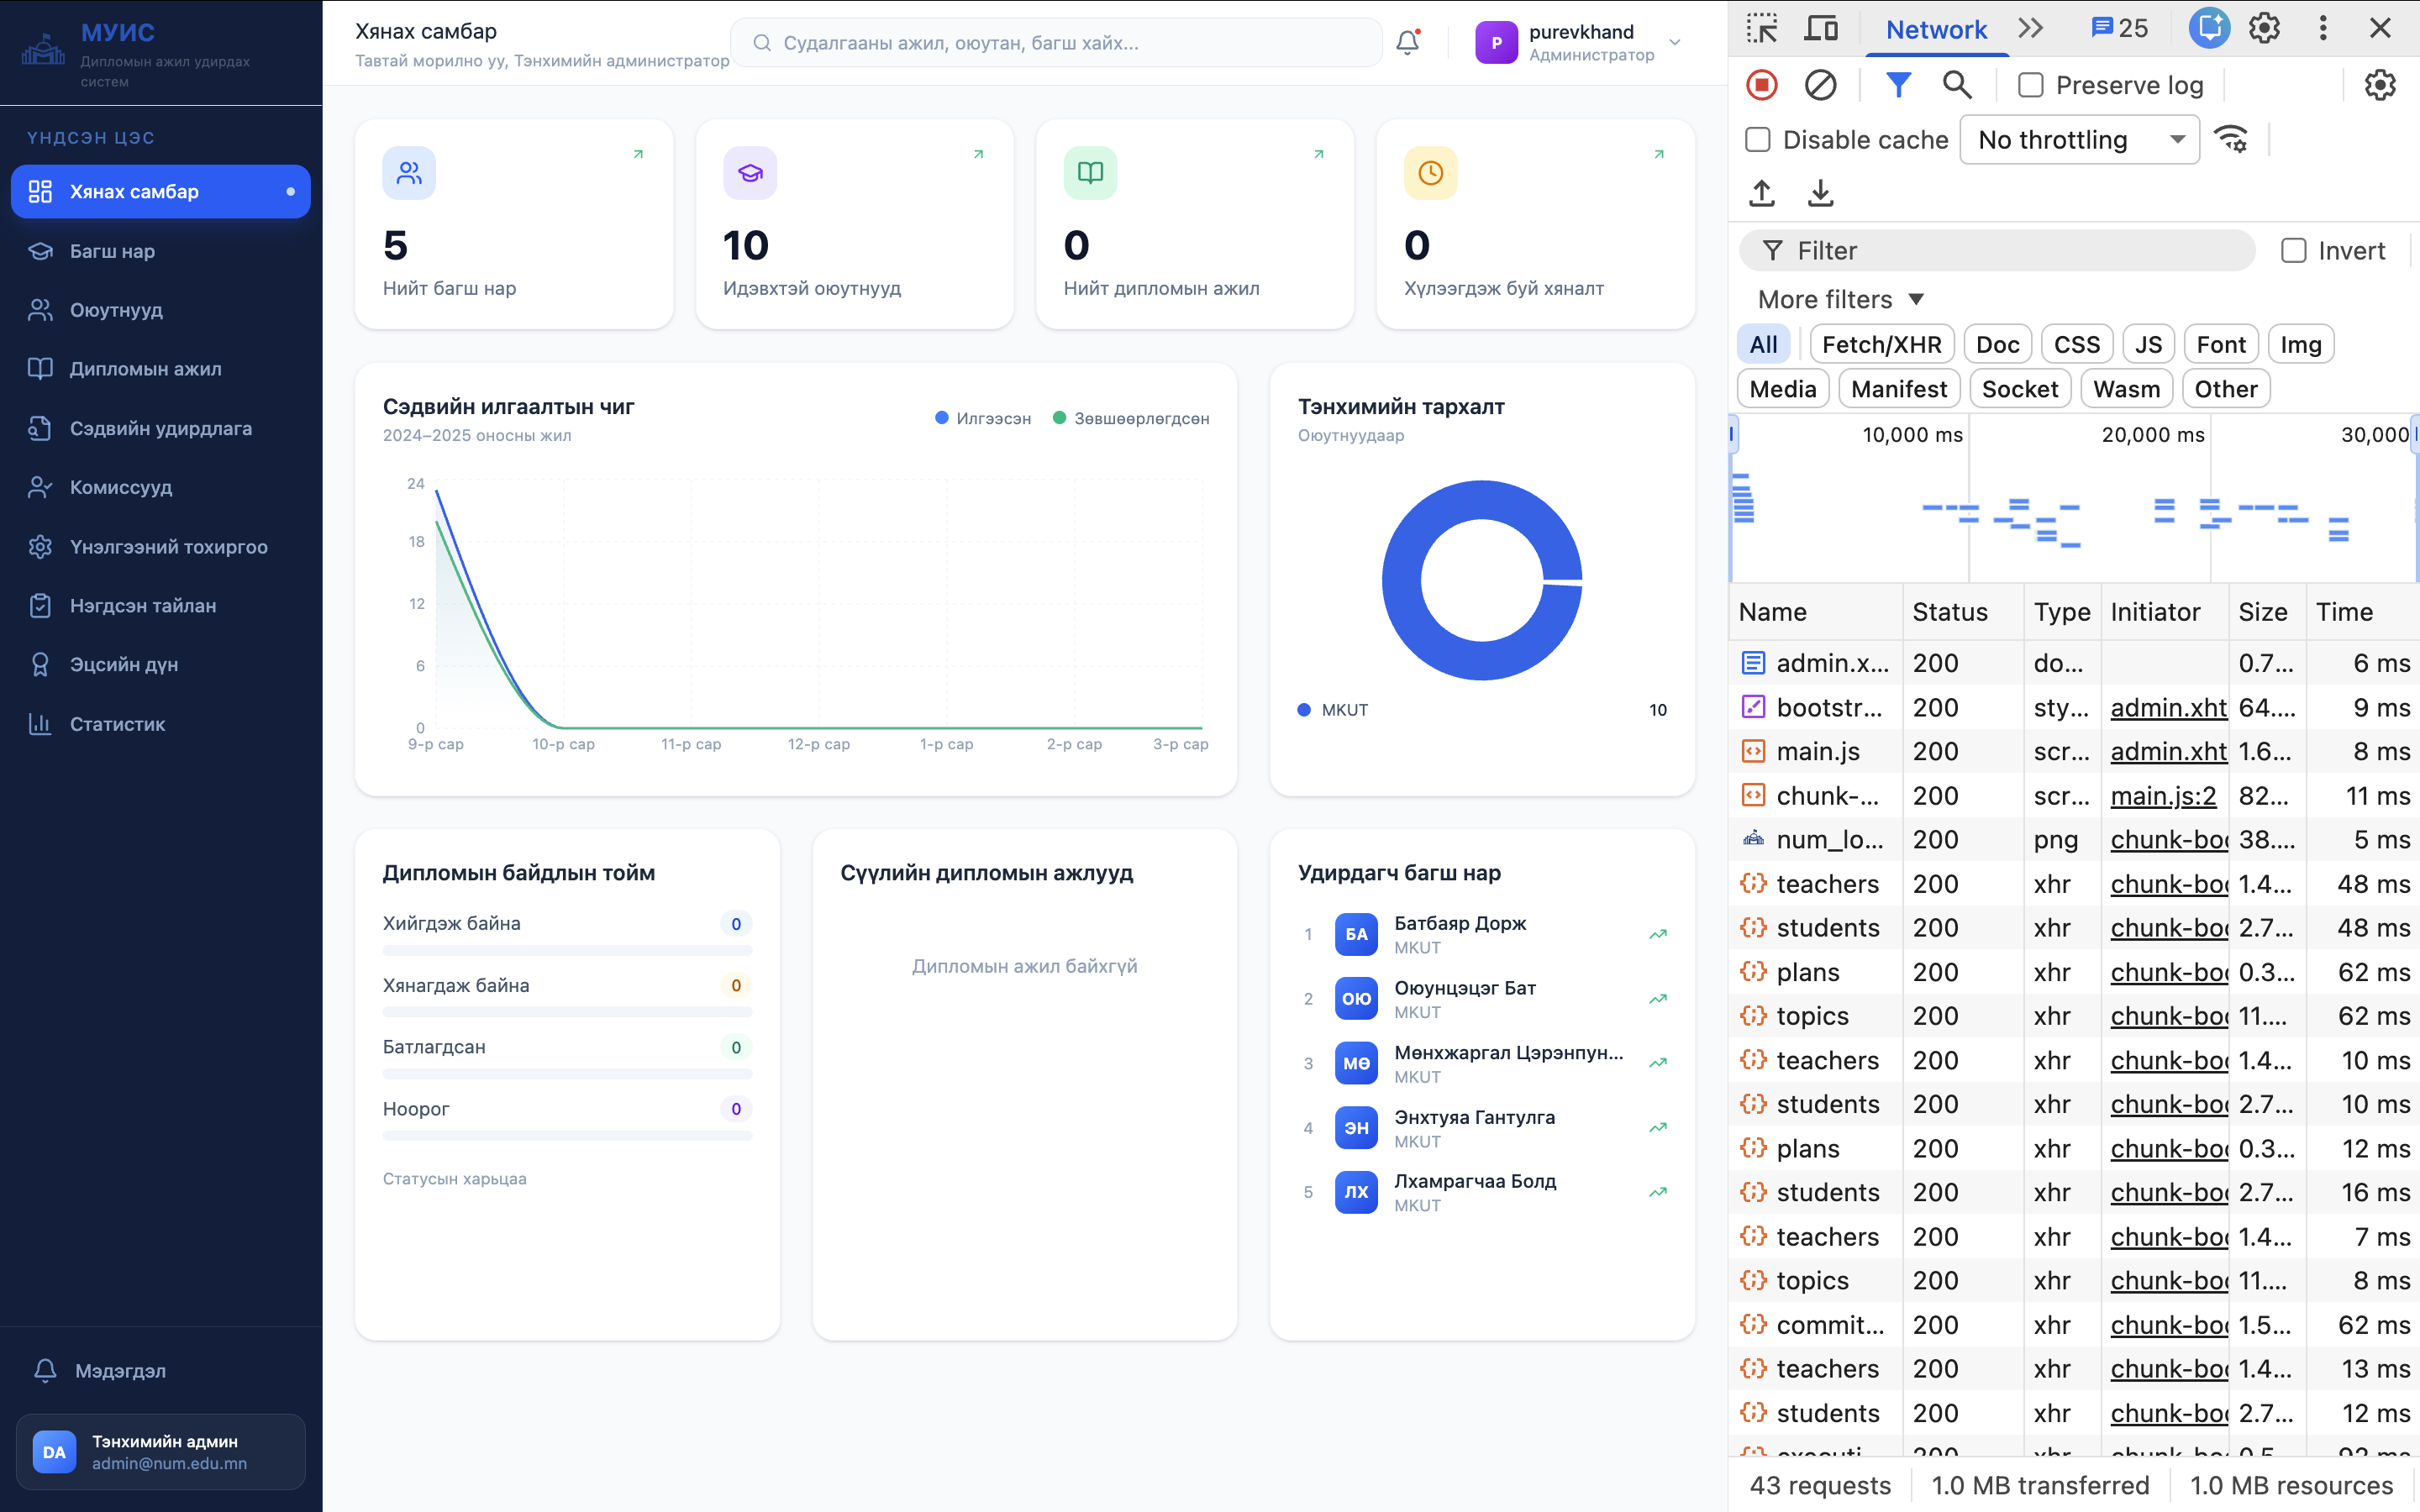
\includegraphics[width=14cm]{images/fig_implementation_summary.png}
    \caption{Зураг 4.10. Системийн хэрэгжүүлэлтийн нэгдсэн бүдүүвч. Frontend MFE давхарга, Tomcat хост, backend микросервис, PostgreSQL өгөгдлийн давхарга нь нэгдсэн байдлаар хамтарч ажилладаг бүрэн дүр зургийг харуулна. Эх сурвалж: зохиогчийн судалгаа, 2026.}
    \label{fig:impl_summary}
\end{figure}
 гэж үндсэн файлд оруулна
% Шаардлагатай package-ууд: booktabs, float, graphicx, listings,
%   tabularx, amsmath, hyperref
% =====================================================================

3-р бүлэгт тодорхойлсон архитектурын загвар нь хийсвэр зарчмуудын
цуглуулга~--- энэхүү бүлэгт эдгээр зарчмуудыг бодит кодын дэс дараа,
тохиргооны файл, алдааны дүн шинжилгээ, инженерчлэлийн практик
шийдлийн хэлбэрт хувиргасан ажлыг баримтжуулна. Загварын ``юу'' нь
хэрэгжүүлэлтийн ``хэрхэн'' болж хувирах явцад тулгарсан техникийн
хүндрэл, нарийн шийдвэр, хийсвэрлэлийн тохируулгуудыг тайлбарлана.

% ─────────────────────────────────────────────────────────────────────
\section{Frontend Хэрэгжүүлэлт ба Нэгтгэлт}
% ─────────────────────────────────────────────────────────────────────

\subsection{Vite Module Federation-ийн Тохиргоо}

3-р бүлэгт Runtime Integration стратегийг сонгосны практик хэрэгжүүлэлт нь
\texttt{@originjs/vite-plugin-federation} хэрэгсэлд тулгуурласан. Уг
хэрэгсэл нь Webpack~5-ийн \texttt{ModuleFederationPlugin}-ийн Vite орчинд
ажилладаг хувилбар бөгөөд \texttt{remoteEntry.js} файл үүсгэж, Remote
MFE-ийн экспортлосон бүрэлдэхүүнүүдийг Host-д ачаалах боломжийг хангана.

MFE модуль тус бүрийн \texttt{vite.config.ts} нь дараах бүтэцтэй тохиргоог
дагана. \texttt{module-thesis} модулийн тохиргоо нь дараах байдалтай:

\begin{figure}[H]
    \centering
    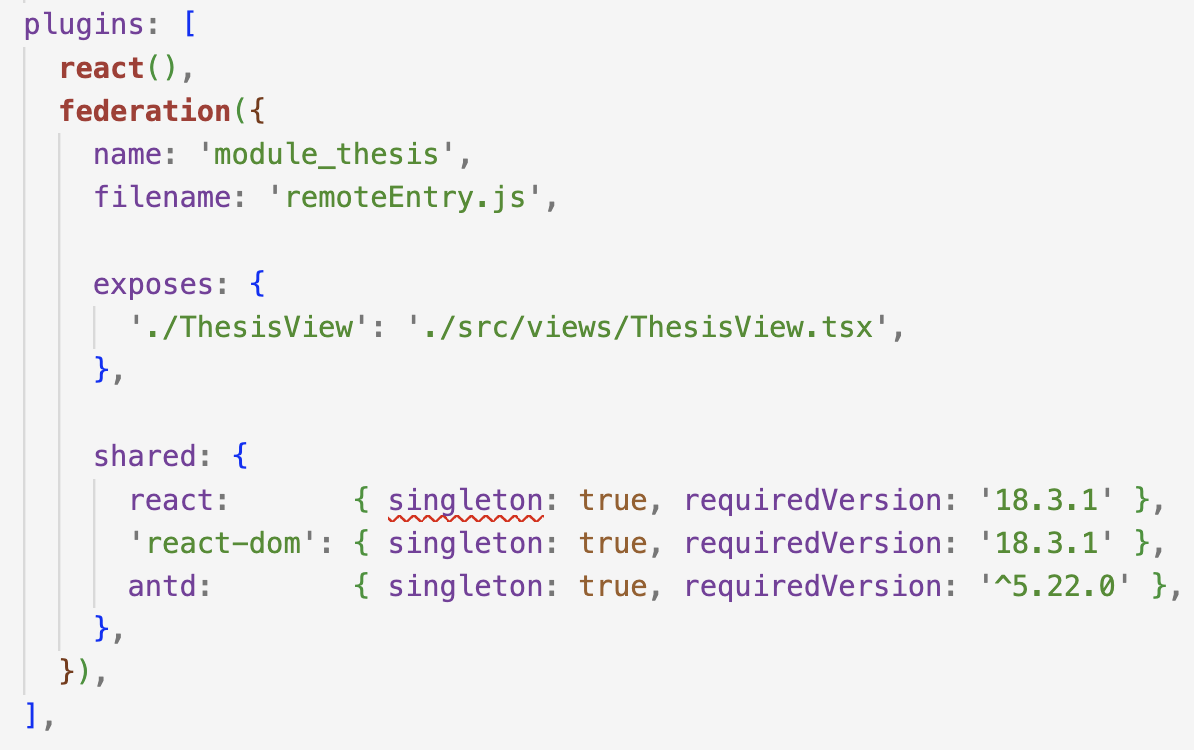
\includegraphics[width=14cm]{images/fig_vite_federation_config.png}
    \caption{Зураг 4.1. \texttt{module-thesis}-ийн \texttt{vite.config.ts} тохиргооны бүтэц. \texttt{name}, \texttt{filename}, \texttt{exposes}, \texttt{shared} дөрвөн гол тохиргооны цэгийг харуулна.}
    \label{fig:vite_config}
\end{figure}

Тохиргооны дөрвөн тулгуур параметрийг тайлбарлая:

\textbf{\texttt{name: 'module\_thesis'}:} Federation-ийн глобал нэрийн
орон зай (namespace). Browser-ийн \texttt{window} объект дээр энэ нэрийн
дор модулийн бүртгэл хийгдэнэ. Нэрийн зөрчлөөс зайлсхийхийн тулд
дор хаяж нэг давхарга нэртэй prefix ашиглах зарчмыг дагав.

\textbf{\texttt{filename: 'remoteEntry.js'}:} Remote MFE-ийн ``агуулгын
хүснэгт'' болох файлын нэр. Host нь энэ URL-г динамикаар \texttt{<script>}
tag хэлбэрт DOM-д оруулах замаар Remote-ийн бүртгэлийг ачаалдаг.

\textbf{\texttt{exposes: \{ './ThesisView': '...' \}}:} Энэ Remote-аас
Host-д нээлттэй байх бүрэлдэхүүнүүд. Дан \texttt{'./ThesisView'} экспортлосон
нь нэгдсэн зарчмыг баримтлж байна~--- нэг Remote нь нэг бизнесийн чадвар.

\textbf{\texttt{shared: \{ react, 'react-dom', antd \}}:} Singleton
хэлбэрт хуваалцагдах хамаарлууд. \texttt{singleton: true} тохиргоо нь
Host болон бүх Remote нэг React instance ашиглахыг баталгаажуулна~---
ингэснээр \texttt{useState}, \texttt{useContext} hook-ууд хөндлөн модулийн
хооронд зөв ажиллана.

\subsection{Runtime Integration: JSF-ийн Script Injection Механизм}

JSF хостын хуудсанд React MFE-г ачаалах гол механизм нь динамик
\texttt{<script>} tag injection юм. Production орчинд Tomcat~8080-д
\texttt{/microfrontends/} замаар static файлуудыг хүргэдэг бол
development орчинд \texttt{http://localhost:30XX} хаягаар Vite-ийн
dev server ажилладаг.

JSF-ийн \texttt{.xhtml} хуудсанд MFE-г ачаалах хэсэг нь дараах
ерөнхий бүтэцтэй:

\begin{figure}[H]
    \centering
    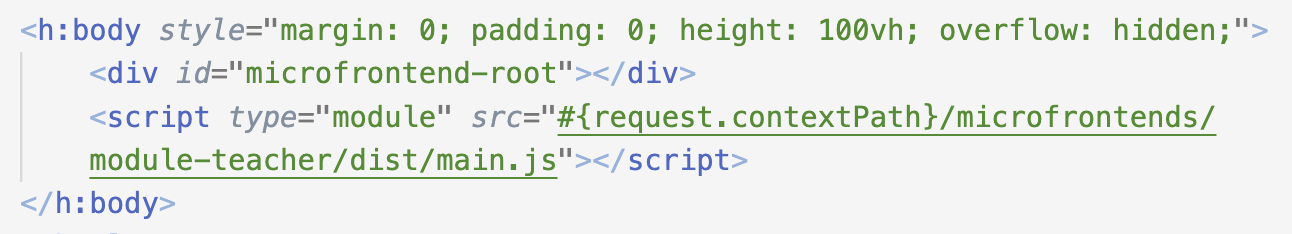
\includegraphics[width=14cm]{images/fig_jsf_script_injection.png}
    \caption{JSF \texttt{.xhtml} хуудасны MFE injection механизм. \texttt{remoteEntry.js} ачаалагдсаны дараа bootstrap.js нь \texttt{<div id="microfrontend-root">} дотор React компонентийг render хийнэ}
    \label{fig:jsf_injection}
\end{figure}

Injection-ийн техникийн дэс дараа:

\begin{enumerate}
  \item JSF Facelets нь хуудсыг server-side render хийхдээ
    \texttt{<div id="microfrontend-root"/>} DOM цэгийг байрлуулна.
  \item \texttt{<script type="module" src=".../remoteEntry.js"/>} tag
    нь браузерт Remote Federation-ийн manifest-ийг ачаална.
  \item \texttt{<script type="module">} блок нь динамик \texttt{import()}
    ашиглан Remote-ийн экспортлосон компонентийг авна.
  \item React-ийн \texttt{createRoot(\#microfrontend-root).render(\ldots)}
    нь тухайн DOM цэгт компонентийг mount хийнэ.
  \item React Router-ийн \textbf{HashRouter} ашигладгийн шалтгаан нь
    JSF-ийн FacesServlet нь \texttt{/student/*} гэх URL pattern-ийг
    хариуцдаг бөгөөд React SPA маршрутлалт нь JSF-тэй зөрчилддгийг
    арилгахын тулд \texttt{/\#/student/dashboard} хэлбэрийн hash-based
    routing хэрэглэнэ.
\end{enumerate}

\subsection{Маршрутлалтын Хүндрэл ба HashRouter Шийдэл}

MFE архитектурт маршрутлалтын хоёр давхарга байдаг: нэгдүгээр давхарга
нь JSF хостын маршрутлалт (\texttt{FacesServlet}-ийн URL pattern), хоёрдугаар
давхарга нь тухайн MFE-ийн React Router дотоод маршрутлалт. Эдгээр хоёр
давхарга зөрчилдөхөд \textbf{``404 Not Found''} буюу JSF-ийн хуудас олдохгүй
алдаа гардаг.

Энэ зөрчлийг шийдвэрлэх хоёр арга байна:

\begin{enumerate}
  \item \textbf{HistoryRouter + Server Catch-all:} Tomcat-д
    \texttt{<url-pattern>/student/*</url-pattern>} бүгдийг нэг JSF
    хуудас руу шилжүүлж, React Router-ийн \texttt{createBrowserRouter}
    ашиглана. Тохиргоо нарийн боловч хэрэглэгчийн URL чухал.
  \item \textbf{HashRouter:} URL-ийн \texttt{\#} хэсэг нь сервер рүү
    хэзээ ч явдаггүй тул JSF-тэй зөрчилддөггүй. React Router-ийн
    \texttt{HashRouter} нь \texttt{/\#/thesis/list} хэлбэрийн URL
    ашиглан дотоод маршрутлалтыг зохицуулна.
\end{enumerate}

Энэ системд \texttt{HashRouter} сонгосны шалтгаан нь: JSF-ийн \texttt{web.xml}
болон \texttt{faces-config.xml}-ийн нарийн URL pattern тохиргоог өөрчлөх
нь монолитийн дотоод урсгалд нөлөөлнө гэсэн эрсдэлтэй байсан тул
хамгийн бага өөрчлөлтийн зарчмаар \texttt{HashRouter}-ийг сонгов.

\subsection{JWT болон Глобал Төлөвийн Хуваалцалт}

JSF хост болон React MFE хоорондын хэрэглэгчийн нэвтрэлтийн мэдлэгийн
хуваалцалт нь архитектурын хамгийн нарийн хэсэг юм. Хэрэглэгч
\texttt{module-auth}-д нэвтрэхэд дараах дараалал гүйцэтгэгдэнэ:

\begin{figure}[H]
    \centering
    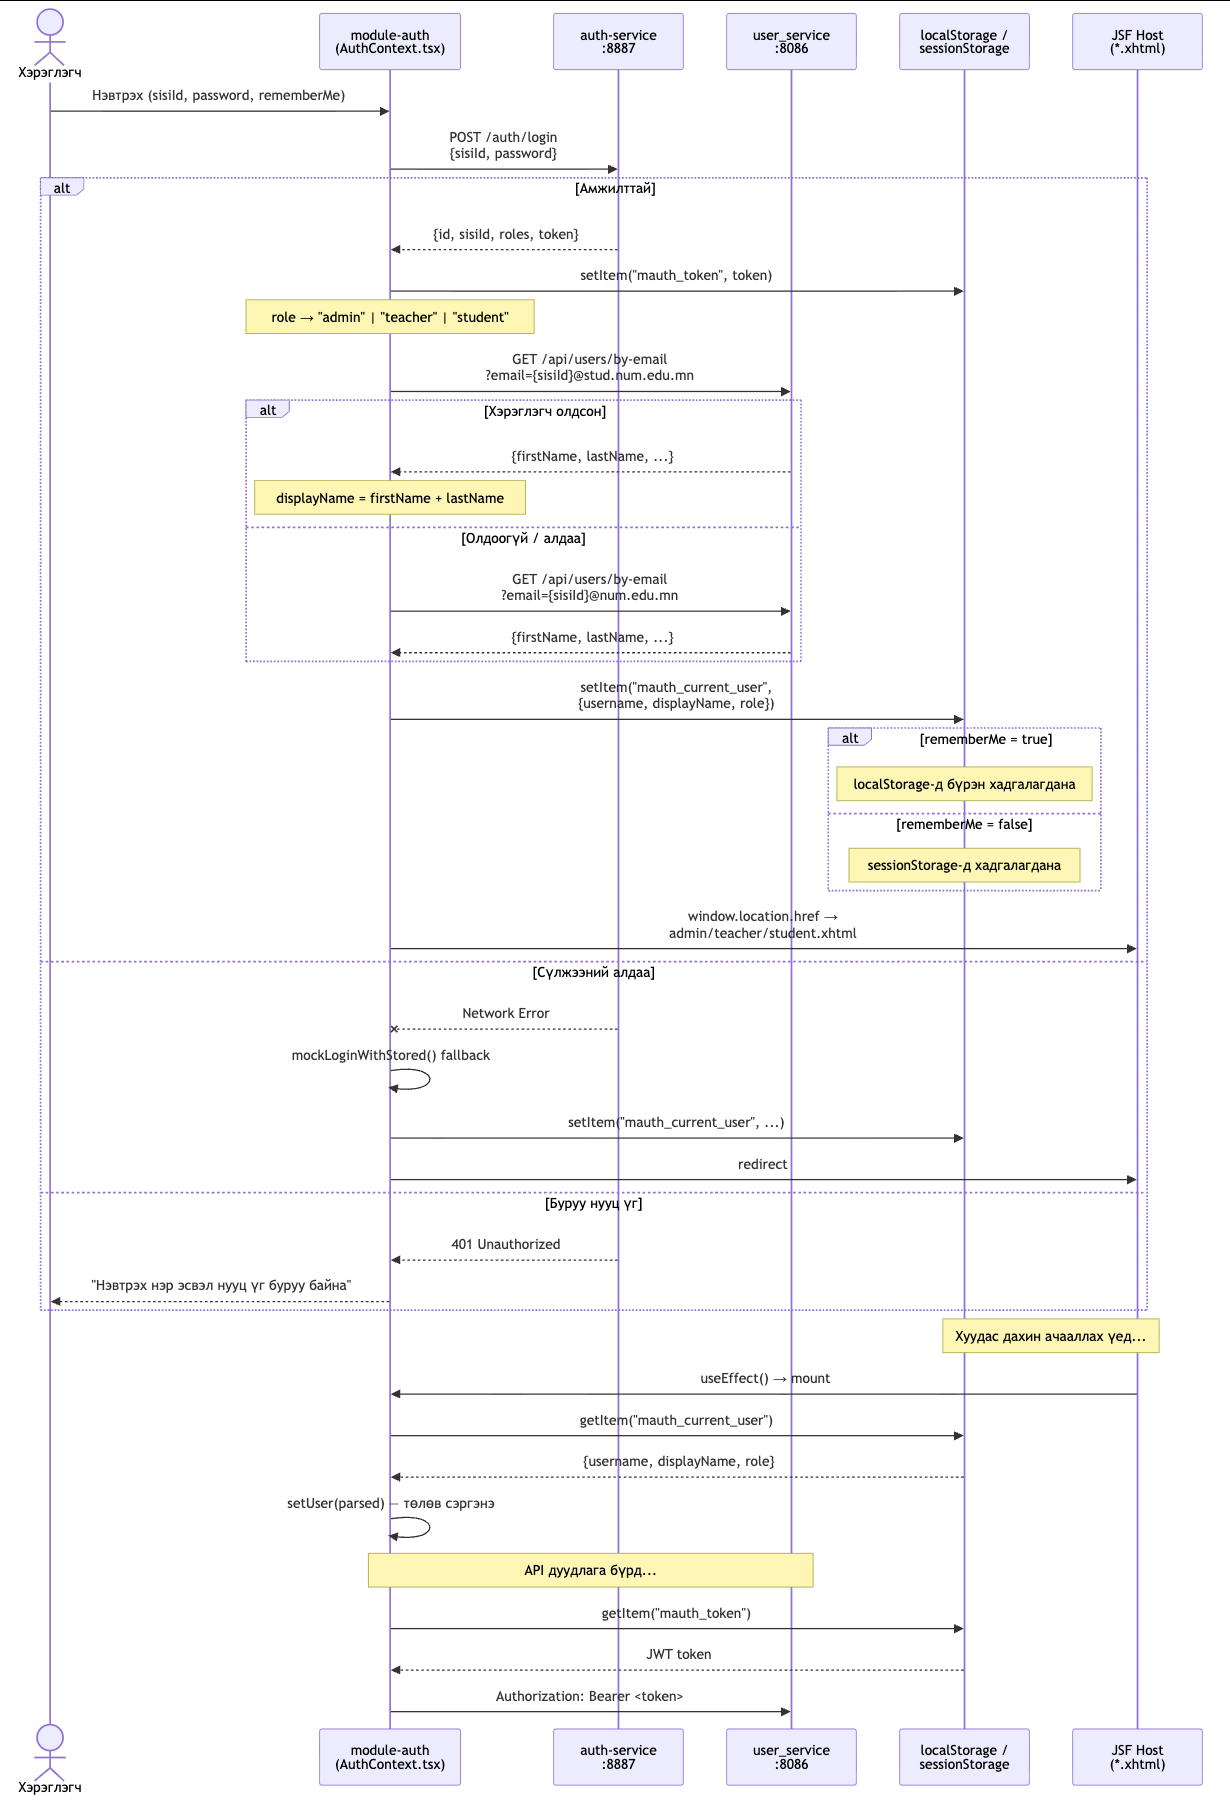
\includegraphics[width=14cm]{images/fig_jwt_flow_sequence.png}
    \caption{JWT нэвтрэлтийн дараалалт диаграм. Auth MFE нь токений хүсэлт илгээж, хүлээн авсан JWT-г localStorage-д хадгалах бөгөөд бусад MFE-ууд нь тэндээс JWT-г уншиж API дуудлагад ашиглана}
    \label{fig:jwt_flow}
\end{figure}

Хуваалцах механизм нь \texttt{localStorage} дотор тодорхой key-д JSON
объект хэлбэрт хадгалагдана:

\begin{itemize}
  \item \texttt{mauth\_token}: JWT Bearer токен~--- API дуудлага бүрийн
    \texttt{Authorization: Bearer \ldots} header-т ашиглагдана.
  \item \texttt{mauth\_current\_user}: \texttt{\{username, displayName,
    role\}} бүтэцтэй JSON~--- хэрэглэгчийн нэр, дүр зэргийг хадгалана.
\end{itemize}

Дизайн шийдвэрийн үндэслэл: \texttt{localStorage} нь хуудас дахин
ачааллагдах (page refresh) болон хэд хэдэн browser tab хооронд бүтэн
хадгалагддаг. \texttt{sessionStorage} нь tab хаагдахад устдаг тул
``Намайг санах'' (Remember Me) функцийг дэмжихгүй. Аюулгүй байдлын
хувьд \texttt{HttpOnly Cookie} нь XSS халдлагаас хамгаалалт сайн боловч
JSF-ийн хуудасны дагуу cookie scope нарийн удирдлага шаардана~---
тул энэ прототипд \texttt{localStorage} ашигласан бөгөөд үйлдвэрлэлийн
орчинд \texttt{HttpOnly} cookie руу шилжихийг зөвлөмж болгоно.

\texttt{AuthContext.tsx} нь React-ийн Context API-д суурилсан global
state provider бөгөөд MFE модуль бүрийн root-д байрладаг. Хуудас
ачааллагдах бүрт localStorage-ийн утгыг уншиж, хэрэглэгчийн төлөвийг
сэргээдэг. Нэвтрэлтийн дараалал нь дараах байна: эхлээд
\texttt{POST http://localhost:8887/auth/login} руу \texttt{\{sisiId,
password\}} илгээнэ; амжилттай тохиолдолд хариуд JWT токен болон
дүрийн мэдээлэл ирнэ; дараа нь \texttt{GET http://localhost:8086/api/users/by-email}
руу хүсэлт илгээж хэрэглэгчийн дэлгэрэнгүй нэрийг авна; эцэст нь
дүрд тохирсон URL руу чиглүүлнэ.

\subsection{Shared-UI ба Singleton Хамаарлын Зохицуулалт}

3-р бүлэгт тодорхойлсон \texttt{shared-ui} модуль нь практик хэрэгжүүлэлтэд
нарийн техникийн хүндрэлтэй тулгарав. Анх nested federation загвараар~---
\texttt{module-thesis} нь \texttt{shared\_ui} Remote-ийг агуулах~---
загварчилсан боловч хэрэгжүүлэлтийн явцад критик алдаа илэрлээ:

\texttt{TypeError: Failed to resolve module specifier '\$\{\_\_federation\_expose\_./SharedUI\}'}

Энэ алдааны үндэс нь \texttt{@originjs/vite-plugin-federation} нь
Remote-ийн \texttt{remoteEntry.js}-д Remote-ийн Remote-ийн URL template-ийг
динамикаар тохируулах механизм дутмаг байдаг явдал юм. Tomcat-д статик
файл хэлбэрт хүргэгдсэн Remote нь өөрийн nested Remote-ийн URL-г
тодорхойлж чадахгүй.

\textbf{Шийдэл:} Nested federation-ийн оронд \texttt{shared-ui}-ийн
бүрэлдэхүүнүүдийг (\texttt{PageHeader}, \texttt{PortalTabs},
\texttt{StatusBadge}, \texttt{DataTable}) тухайн Remote-ийн дотор шууд
нэгтгэж, Ant Design-ийг federation-ийн \texttt{shared singleton}
механизмаар хуваалцана. Энэ нь кодын хуулбарлалтын зардалтай боловч
runtime-д нэг antd instance ашиглагддаг тул bundle хэмжээ нэмэгдэхгүй.

\begin{figure}[H]
    \centering
    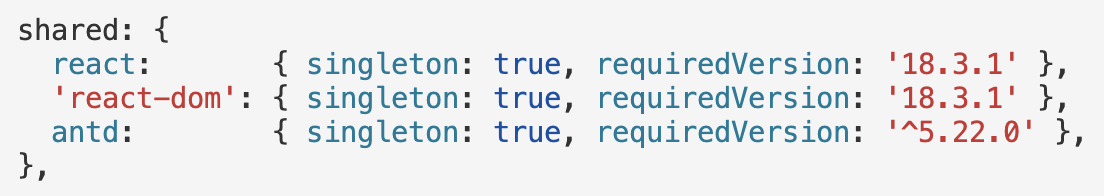
\includegraphics[width=14cm]{images/fig_shared_singleton_pattern.png}
    \caption{Shared Singleton загварын зохицуулалт. Antd нь нэгдсэн singleton хэлбэрт ачааллагдаж, Remote модуль бүр энэ нэг instance-ийг ашиглана~--- nested federation-ийн алдааг арилгана. Эх сурвалж: зохиогчийн судалгаа, 2026.}
    \label{fig:shared_singleton}
\end{figure}

\subsection{Build ба Deploy Паплайн}

Хэрэгжүүлэлтийн орчинд \texttt{build-modules.sh} shell скрипт нь
бүх MFE модулийг дараалан build хийж, \texttt{dist/} гаралтыг
Tomcat-ийн \texttt{webapps/microfrontends/\{module-name\}/dist/}
хавтаст хуулдаг. Скриптийн ерөнхий урсгал нь:

\begin{enumerate}
  \item MFE модуль бүрийн \texttt{npm run build} ажиллуулна.
  \item \texttt{dist/assets/remoteEntry.js} файлыг \texttt{dist/}
    root рүү хуулна~--- \texttt{@originjs}-ийн хуучин хувилбар нь
    \texttt{remoteEntry.js}-г \texttt{dist/assets/} дотор үүсгэдэг
    тул Host-ийн URL тохиргоотой зөрчилддгийг засна.
  \item Томкат нь \texttt{/microfrontends/\{module\}/dist/remoteEntry.js}
    замаар тухайн Remote-ийн manifest-ийг хүргэнэ.
\end{enumerate}

\begin{figure}[H]
    \centering
    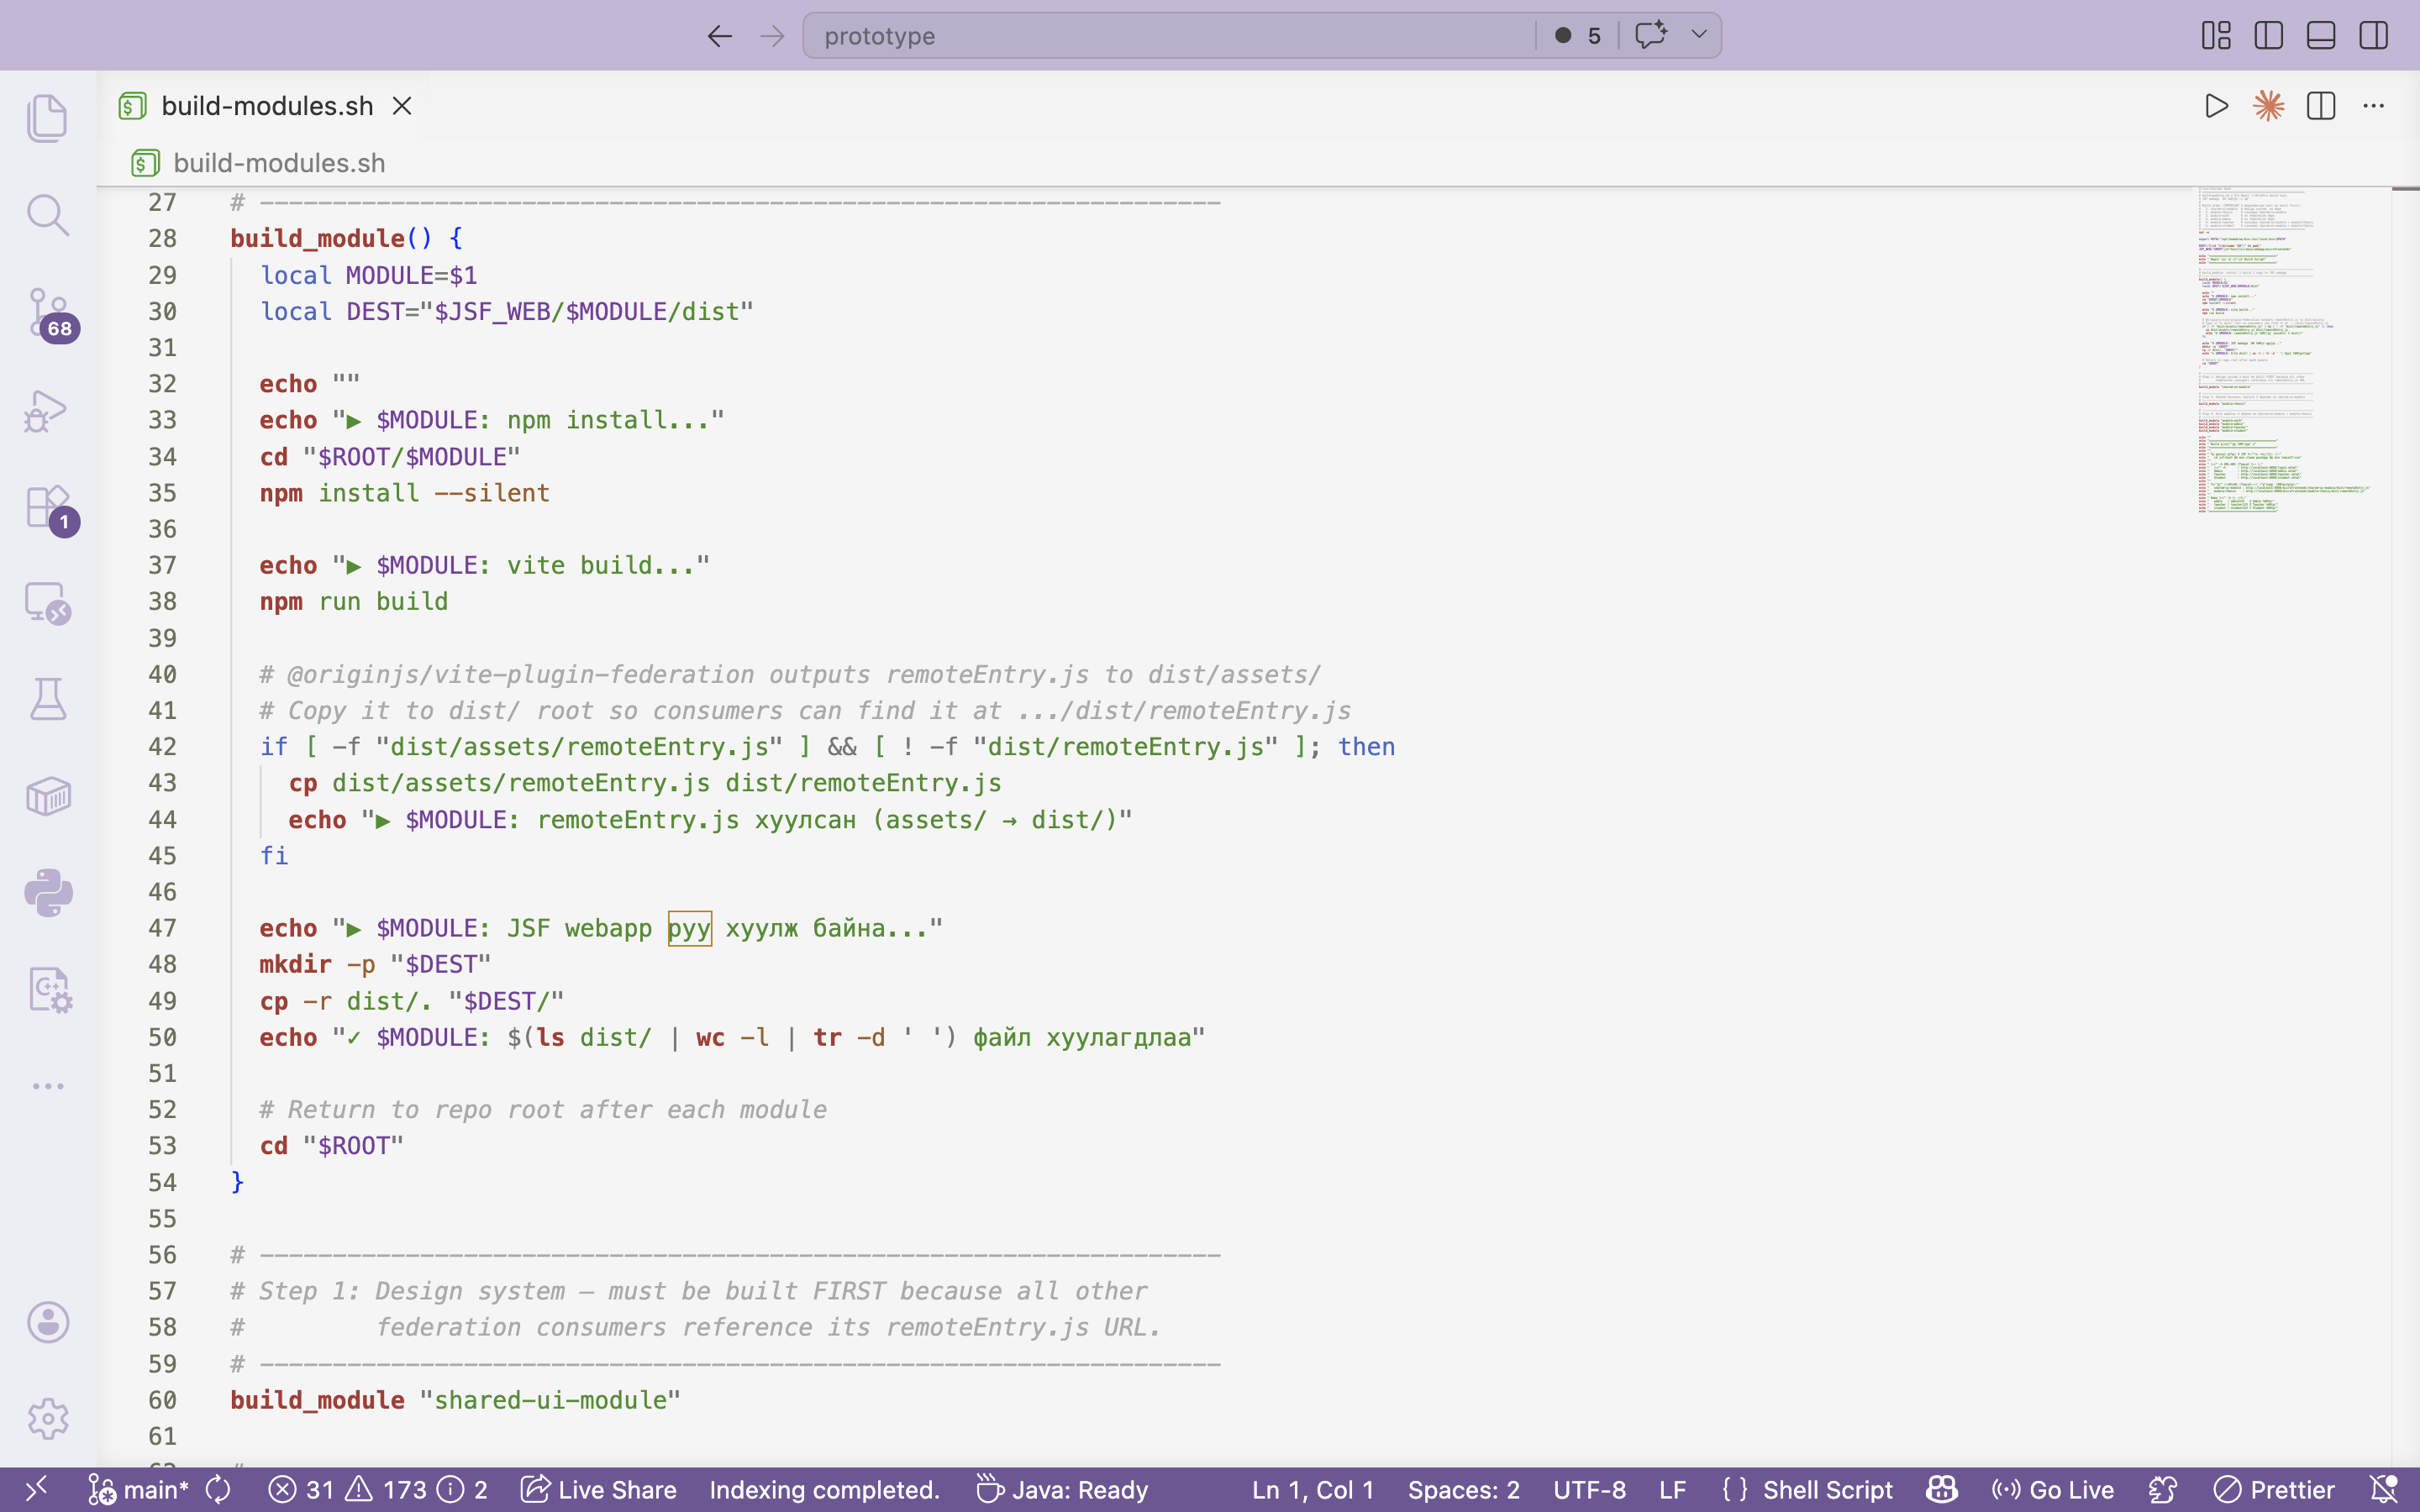
\includegraphics[width=14cm]{images/fig_build_deploy_pipeline.png}
    \caption{Зураг 4.5. Build ба Deploy паплайны урсгалын диаграм. Модуль тус бүрийн Vite build гаралт нь Tomcat-ийн webapps хавтасрт хуулагдаж, нэгдсэн байдлаар 8080 порт дээр хүргэгдэнэ. Эх сурвалж: зохиогчийн судалгаа, 2026.}
    \label{fig:build_pipeline}
\end{figure}

% ─────────────────────────────────────────────────────────────────────
\section{Backend Хэрэгжүүлэлт}
% ─────────────────────────────────────────────────────────────────────

\subsection{Spring Boot болон Spring WebFlux-ийн Сонголт}

Backend микросервисүүдийн хэрэгжүүлэлтэд Java~21 болон Spring Boot~3.2.x
framework-ийг ашиглав. Гэвч 3-р бүлгийн 3.3.2-т тодорхойлсон масштабдах
чадварын шаардлагын дагуу уламжлалт \textbf{Spring MVC} (thread-per-request)
загварын оронд \textbf{Spring WebFlux} (reactive, event-loop) загварыг
сонгов.

Spring MVC нь request бүрт нэг thread хуваарилдаг тул 1,000 зэрэгцэх
хүсэлт нь 1,000 thread шаарддаг~--- JVM-ийн thread stack дундажаар 512~КБ
тул 1,000 thread нь $\approx$~500~МБ санах ой хэрэглэнэ. Spring WebFlux
нь Netty-ийн Non-blocking I/O event-loop дээр суурилж, CPU-ийн цөмийн
тоо ($n$) thread-аар хэдэн мянган зэрэгцэх холболтыг удирддаг.

\textbf{Hexagonal Architecture (Ports and Adapters):} Сервис тус бүрийн
дотоод бүтэц нь Alistair Cockburn (2005)-ийн Hexagonal Architecture
зарчмаар зохион байгуулагдсан:

\begin{itemize}
  \item \textbf{Domain Layer:} Бизнесийн логик агуулсан цөм~---
    жишээ нь \texttt{Thesis}, \texttt{WorkflowState} домейн объектууд.
    Аль ч фреймворкоос тусгаарлагдсан цэвэр Java/Kotlin класс.
  \item \textbf{Application Layer (Ports):} Use Case интерфэйс~---
    \texttt{CreateStudentUseCase}, \texttt{FindUserUseCase},
    \texttt{SubmitThesisUseCase}. Домейн логикийг хэрхэн дуудах
    гэрээг тодорхойлно.
  \item \textbf{Adapter Layer:} Гадаад ертөнцтэй холбогч~---
    \texttt{UserController} (HTTP adapter), \texttt{UserR2dbcRepository}
    (persistence adapter), \texttt{NotificationWebSocketAdapter}
    (messaging adapter).
\end{itemize}

\begin{figure}[H]
    \centering
    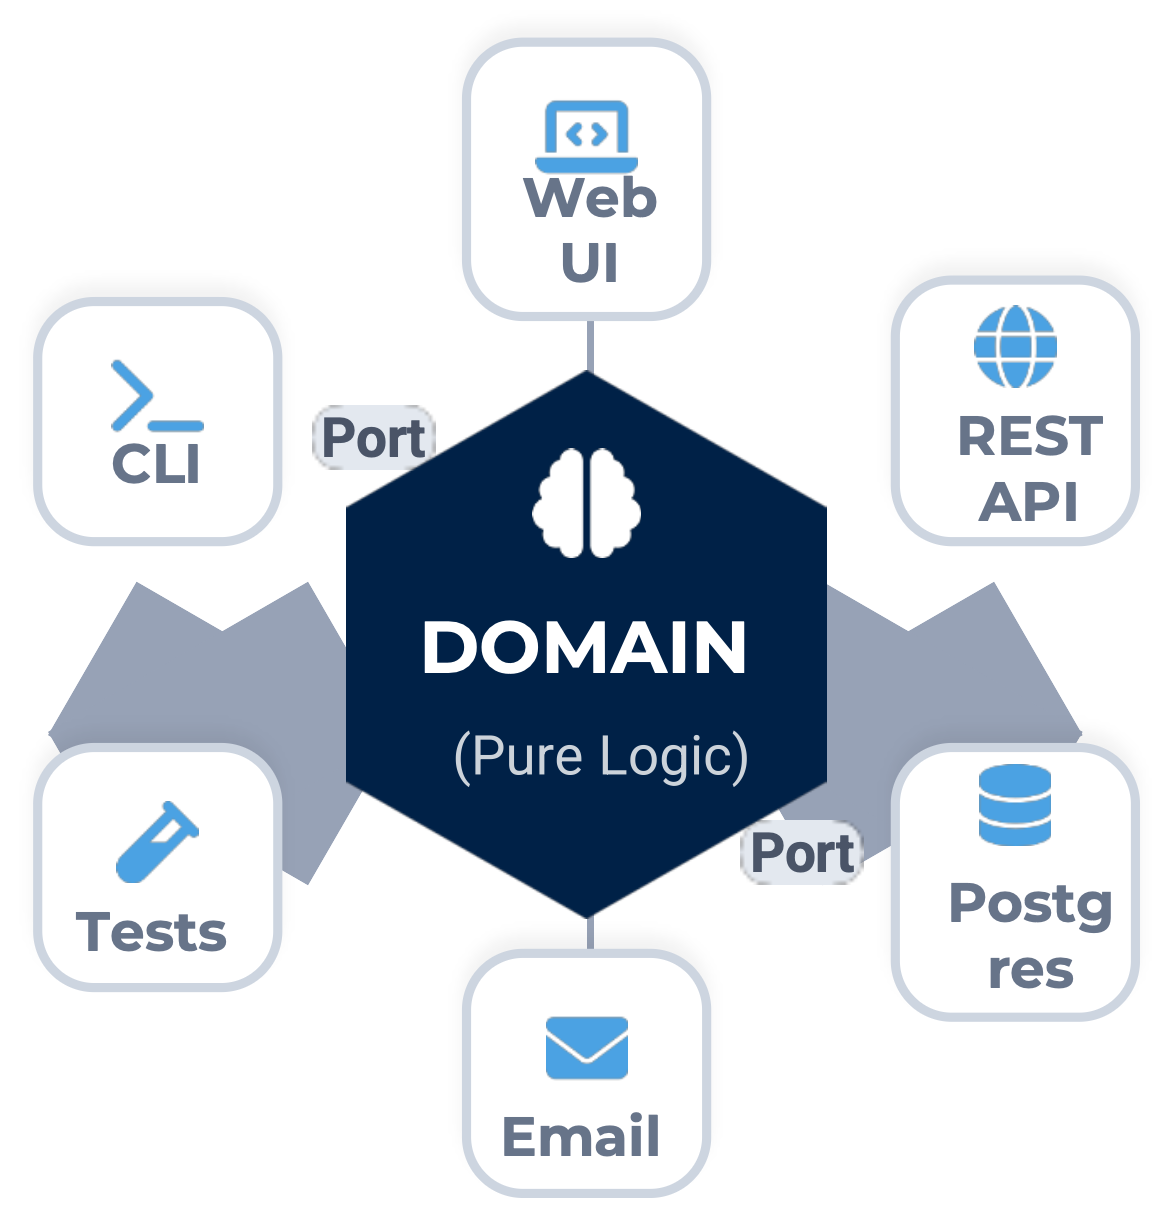
\includegraphics[width=14cm]{images/fig_hexagonal_architecture.png}
    \caption{Hexagonal Architecture-ийн \texttt{user\_service} дахь хэрэгжүүлэлтийн бүтэц. Домейн давхарга нь дотор цагирагт, Port-ууд нь дунд цагирагт, Adapter-ууд нь гадаад цагирагт байрлана. Эх сурвалж: зохиогчийн судалгаа, 2026.}
    \label{fig:hexagonal_arch}
\end{figure}

\subsection{Микросервис Тус Бүрийн Хэрэгжүүлэлтийн Нарийн}

\subsubsection{auth-service ба JWT Токений Хэрэгжүүлэлт}

\texttt{auth-service} нь \texttt{sisiId} болон нууц үг хүлээн авч, хэрэглэгчийн
бичлэгтэй харьцуулж, \texttt{jjwt}~(Java JWT) санг ашиглан токен
үүсгэнэ. Токений payload нь \texttt{\{sub: sisiId, roles: [...],
iat: epochSeconds, exp: iat+86400\}} бүтэцтэй. Нийтийн болон хувийн
түлхүүрийн хос (RSA-256)-ийн оронд энэ прототипд HMAC-SHA256 алгоритмтай
нийтлэг нууц key ашиглагдав~--- үйлдвэрлэлийн орчинд RSA key pair
болон Key Management Service (KMS) ашиглахыг зөвлөмж болгоно.

\texttt{authorization-service} нь дүр болон эрхийн матрицийг удирдана.
\texttt{ROLE\_ADMIN}, \texttt{ROLE\_TEACHER}, \texttt{ROLE\_STUDENT},
\texttt{ROLE\_COMMITTEE\_MEMBER} дүрүүд тодорхойлогдсон бөгөөд endpoint
бүр дээр Spring Security-ийн \texttt{@PreAuthorize} annotationоор
хандах эрхийн шалгалт хэрэгжинэ.

\subsubsection{user\_service-ийн Reactive Хэрэгжүүлэлт}

\texttt{user\_service} нь Spring WebFlux болон R2DBC-г хослуулан ашиглах
бөгөөд \texttt{UserController}-д хэрэглэгчийн CRUD болон хайлтын
endpoint-ууд хэрэгждэнэ. \texttt{/api/users/by-email} endpoint нь
\texttt{UserR2dbcRepository.findByEmail(String email)} reactive метод
дуудаж, \texttt{Mono<User>} буцаана~--- энэ нь AuthContext-ийн
display name lookup-д зориулан нэмэгдсэн.

\texttt{UserR2dbcRepository} нь \texttt{ReactiveCrudRepository<User, String>}
интерфэйсийг өргөтгөсөн бөгөөд Spring Data R2DBC нь SQL query-г
\texttt{findBy\{FieldName\}} нэрлэлтийн конвенцоос автоматаар үүсгэнэ.
Энэ нь ``конвенц дагасан тохиргоо'' (convention over configuration)
зарчмын практик хэрэглэлт бөгөөд boilerplate кодын хэмжээг мэдэгдэхүйц
бууруулна.

\subsubsection{workflow\_service-ийн State Machine Хэрэгжүүлэлт}

\texttt{workflow\_service} нь дипломын ажлын статус шилжилтийг хариуцна.
State Machine нь Java-ийн enum болон явцын хамгаалагдсан шилжилтийн
матрицаар хэрэгжинэ:

\begin{table}[H]
    \centering
    \caption{Дипломын ажлын статус шилжилтийн зөвшөөрөгдсөн матриц}
    \label{tab:workflow_transitions}
    \renewcommand{\arraystretch}{0.7}
    \begin{tabular}{lll}
        \toprule
        \textbf{Одоогийн статус} & \textbf{Зорилтот статус} & \textbf{Хэн гүйцэтгэх} \\
        \midrule
        DRAFT              & SUBMITTED           & Оюутан \\
        SUBMITTED          & UNDER\_REVIEW       & Удирдагч багш \\
        SUBMITTED          & REJECTED            & Удирдагч багш \\
        UNDER\_REVIEW      & REVISION\_REQUESTED & Удирдагч багш \\
        UNDER\_REVIEW      & APPROVED            & Удирдагч багш \\
        REVISION\_REQUESTED & SUBMITTED          & Оюутан \\
        APPROVED           & DEFENSE\_SCHEDULED  & Систем / Админ \\
        DEFENSE\_SCHEDULED & DEFENDED            & Хорооны гишүүн \\
        DEFENDED           & ARCHIVED            & Систем \\
        \bottomrule
    \end{tabular}
\end{table}

Зөвшөөрөгдөөгүй шилжилтийн оролдлого нь \texttt{HTTP 422 Unprocessable
Entity} буцаах бөгөөд хариу body нь шилжилт яагаад зөвшөөрөгдөхгүй
байгаа шалтгааны тайлбарыг агуулна.

\subsection{API Gateway-ийн Тохиргоо}

Тус системд тусдаа API Gateway сервис биш харин \textbf{Tomcat-ийн
reverse proxy} тохиргоо gateway-ийн үүрэг гүйцэтгэнэ. Apache Tomcat
нь \texttt{server.xml}-д \texttt{ProxyPass} директивоор (эсвэл Nginx
reverse proxy хослуулан) backend сервисүүд рүү HTTP хүсэлтийг
чиглүүлнэ. Энэ нь Nginx эсвэл Spring Cloud Gateway-тай харьцуулахад
хялбар боловч илүү нарийн CORS, rate limiting, circuit breaker
хяналт шаарддаг тул ирээдүйн шатанд тусдаа gateway нэвтрүүлэх
хэрэгцээ байна.

Frontend JavaScript-аас API дуудлагын CORS тохиргоо нь сервис
бүрийн \texttt{application.yml}-д тохируулагдсан:

\begin{figure}[H]
    \centering
    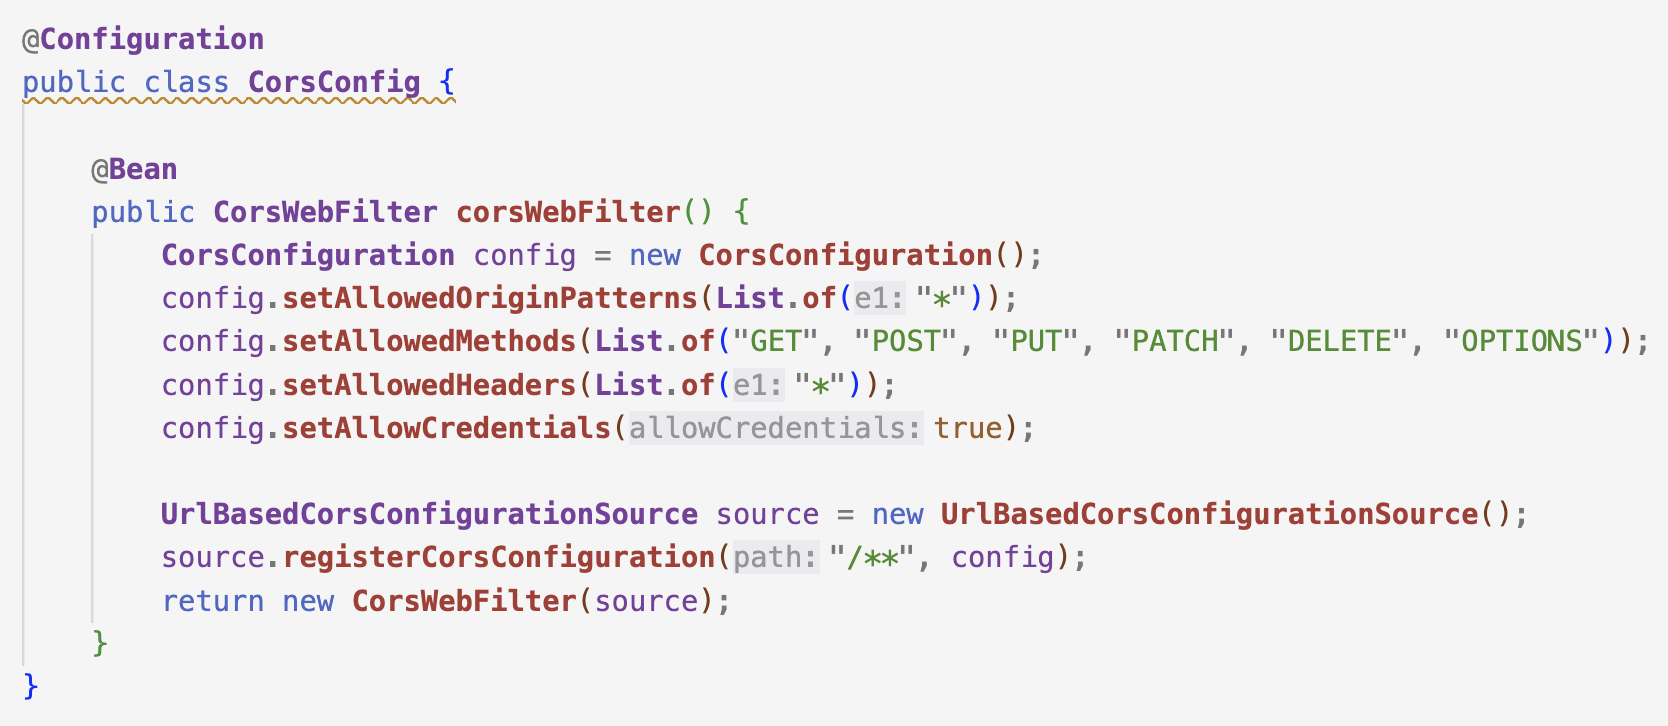
\includegraphics[width=14cm]{images/fig_cors_config.png}
    \caption{Зураг 4.7. Spring WebFlux-ийн CORS тохиргооны жишээ. \texttt{allowedOrigins} нь Tomcat-ийн 8080 порт, \texttt{allowedMethods} нь REST стандартын бүх method-уудыг агуулна. Эх сурвалж: зохиогчийн судалгаа, 2026.}
    \label{fig:cors_config}
\end{figure}

\texttt{allowedOrigins: "http://localhost:8080"} нь зөвхөн JSF хостын
хаягаас ирсэн AJAX хүсэлтийг зөвшөөрнө. Үйлдвэрлэлийн орчинд
энэ нь бодит domain нэрийг агуулна, wildcard (\texttt{*}) ашиглахаас
зайлсхийнэ.

\subsection{Distributed Tracing-ийн Хэрэгжүүлэлт}

Сервисүүдийн хоорондох хүсэлтийн урсгалыг хянах Distributed Tracing-ийг
OpenTelemetry Java Agent болон Jaeger-ийн хослолоор хэрэгжүүлэв.
JVM startup parameter-т \texttt{-javaagent:opentelemetry-agent.jar}
нэмснээр application кодыг өөрчлөхгүйгээр HTTP request бүрт
\texttt{traceparent}, \texttt{tracestate} W3C стандартын trace header
автоматаар нэмэгдэнэ.

Нэг хэрэглэгчийн хүсэлт хэд хэдэн сервисийг дамжих бүрт нэг
\texttt{traceId}-ийн дор бүх span-ууд нэгтгэгдэнэ~--- Jaeger UI-д
waterfall диаграм хэлбэрт харагддаг бөгөөд сервис бүрийн саатал
(latency contribution) тус тусад нь хэмжигдэнэ. Оюутан дипломын ажил
илгээхэд \texttt{POST /api/thesis/submit}-ийн trace нь
\texttt{auth-service} (JWT шалгах), \texttt{thesis-service}
(бичлэг шинэчлэх), \texttt{workflow-service} (статус шилжүүлэх),
\texttt{notification-service} (мэдэгдэл илгээх) гэсэн 4 span агуулдаг.

% ─────────────────────────────────────────────────────────────────────
\section{Өгөгдлийн Сангийн Хэрэгжүүлэлт}
% ─────────────────────────────────────────────────────────────────────

\subsection{PostgreSQL болон R2DBC-ийн Сонголт}

3-р бүлгийн өгөгдлийн давхаргын загварчлалд PostgreSQL-г харилцааны
(relational) өгөгдлийн санаар, R2DBC-г реактив driver хэлбэрт сонгосон
байсан. Практик хэрэгжүүлэлтэд PostgreSQL~16.2 болон
\texttt{io.r2dbc:r2dbc-postgresql:1.0.4} driver ашиглав.

\textbf{Яагаад PostgreSQL:} Дипломын ажлын бизнесийн логик нь олон
харилцаатай өгөгдлийн бүтэц (User $\leftrightarrow$ Thesis
$\leftrightarrow$ Committee $\leftrightarrow$ Evaluation) агуулдаг
тул харилцааны бүрэн бүтэн байдлын баталгаа (referential integrity),
ACID transaction, SQL-ийн хүчирхэг query боломж шаардагдана. Document
store (MongoDB) нь schema-flexible боловч JOIN-ийн хэрэгцээтэй энэ
домейнд неудобен.

\textbf{Яагаад R2DBC (JDBC биш):} Spring WebFlux-ийн event-loop
загвар нь blocking JDBC дуудлагатай ``reactive pollution'' (цуваа
блоклолт) асуудалд орно~--- blocking call нь event-loop thread-ийг
хааж, бусад хүсэлтийн хариулт удаашралд орно. R2DBC нь Non-blocking
reactive driver тул WebFlux-тэй зохистой хэрэгждэнэ.

\subsection{Schema Тодорхойлолт ба Migration}

Сервис тус бүрийн өгөгдлийн сангийн schema нь тухайн сервисийн
\texttt{src/main/resources/schema\_\{service\_name\}.sql} файлд
тодорхойлогдсон. Эхний нэвтрэлтэд Spring Boot-ийн
\texttt{spring.sql.init.mode: always} тохиргоог ашиглан schema
автоматаар үүснэ. Үйлдвэрлэлийн орчинд Flyway эсвэл Liquibase
migration хэрэгслийг ашиглахыг зөвлөмж болгоно.

\texttt{user\_service}-ийн \texttt{schema\_user\_service.sql}-ийн
гол хэсгийг жишээ болгон дурдвал:

\begin{lstlisting}[language=sql, caption={\texttt{user\_service}-ийн SQL schema-ийн жишээ. \texttt{users}, \texttt{departments} хүснэгтүүдийн DDL болон constraint-уудыг харуулна.}, label={lst:schema_sql}]
CREATE TABLE IF NOT EXISTS users (
    id              VARCHAR(255) PRIMARY KEY,
    first_name      VARCHAR(255) NOT NULL,
    last_name       VARCHAR(255) NOT NULL,
    email           VARCHAR(255) NOT NULL UNIQUE,
    department_id   VARCHAR(255),
    system_role     VARCHAR(50)  NOT NULL,
    active          BOOLEAN      NOT NULL DEFAULT TRUE,
    photo_url       VARCHAR(1000),
    created_at      TIMESTAMP    NOT NULL DEFAULT CURRENT_TIMESTAMP,
    CONSTRAINT chk_system_role
        CHECK (system_role IN ('ADMIN','STUDENT','TEACHER','DEPARTMENT_HEAD'))
);

CREATE TABLE IF NOT EXISTS students (
    id                  VARCHAR(255) PRIMARY KEY,
    user_id             VARCHAR(255) NOT NULL UNIQUE
        REFERENCES users(id) ON DELETE CASCADE,
    student_id          VARCHAR(255) NOT NULL UNIQUE,  
    major               VARCHAR(255),
    has_approved_topic  BOOLEAN NOT NULL DEFAULT FALSE
);

CREATE TABLE IF NOT EXISTS teachers (
    id                          VARCHAR(255) PRIMARY KEY,
    user_id                     VARCHAR(255) NOT NULL UNIQUE
        REFERENCES users(id) ON DELETE CASCADE,
    position                    VARCHAR(255),
    supervisor_quota            INT NOT NULL DEFAULT 5,
    current_supervised_count    INT NOT NULL DEFAULT 0,
    CONSTRAINT chk_quota_positive
        CHECK (supervisor_quota > 0),
    CONSTRAINT chk_count_non_negative
        CHECK (current_supervised_count >= 0)
);

CREATE TABLE IF NOT EXISTS departments (
    id              VARCHAR(255) PRIMARY KEY,
    user_id         VARCHAR(255) NOT NULL UNIQUE
        REFERENCES users(id) ON DELETE CASCADE,
    department_name VARCHAR(255) NOT NULL
);
CREATE INDEX IF NOT EXISTS idx_users_email       ON users(email);
CREATE INDEX IF NOT EXISTS idx_users_role        ON users(system_role);
CREATE INDEX IF NOT EXISTS idx_users_dept        ON users(department_id);
CREATE INDEX IF NOT EXISTS idx_students_user     ON students(user_id);
CREATE INDEX IF NOT EXISTS idx_students_sisi     ON students(student_id);
CREATE INDEX IF NOT EXISTS idx_teachers_user     ON teachers(user_id);
CREATE INDEX IF NOT EXISTS idx_departments_user  ON departments(user_id);

\end{lstlisting}

\texttt{user\_type} нь PostgreSQL-ийн native \texttt{ENUM} гэхийн
оронд \texttt{VARCHAR(20) CHECK (user\_type IN (...))}-ийн хэлбэрт
хэрэгжсэн~--- R2DBC-ийн хуучин хувилбарт native enum-ийн codec
авторегистр хийгддэггүй тул энэ шийдэл нь портатив, хамааралгүй.

\subsection{Connection Pooling ба Гүйцэтгэлийн Тохируулга}

R2DBC нь өөрийн \texttt{r2dbc-pool} connection pool-тай. Сервис
тус бүрийн \texttt{application.yml}-д connection pool-ийн тохиргоо
дараах байдлаар хийгдэв:

\begin{table}[H]
    \centering
    \caption{R2DBC Connection Pool-ийн тохиргооны параметрүүд}
    \label{tab:r2dbc_pool}
    \renewcommand{\arraystretch}{0.7}
    \begin{tabular}{lrl}
        \toprule
        \textbf{Параметр} & \textbf{Утга} & \textbf{Тайлбар} \\
        \midrule
        \texttt{initial-size}       & 5   & Эхлэлийн холболтын тоо \\
        \texttt{max-size}           & 20  & Хамгийн их зэрэгцэх холболт \\
        \texttt{max-idle-time}      & 30м & Идэвхгүй холболтын хамгийн их хугацаа \\
        \texttt{max-life-time}      & 60м & Холболтын нийт амьдах хугацаа \\
        \texttt{acquire-retry}      & 3   & Холболт авах оролдлогын тоо \\
        \texttt{validation-query}   & SELECT~1 & Холболт шалгах query \\
        \bottomrule
    \end{tabular}
\end{table}

\texttt{max-size: 20} нь нэг PostgreSQL-ийн default \texttt{max\_connections}
(100)-тай харьцуулахад таван сервис нэгэн зэрэг ажиллахад нийт
$5 \times 20 = 100$ холболтын хязгаарт ойрхон болно. Үйлдвэрлэлийн
орчинд \texttt{pgBouncer} connection pooler нэмэх нь PostgreSQL-ийн
connection-г дахин ашиглах боломж олгоно.

\subsection{Cross-Service Мэдээллийн Нийцэл}

Практик хэрэгжүүлэлтэд distributed transaction (2PC) ашиглахын оронд
дараах хоёр механизмыг хэрэглэв:

\textbf{Application-level Retry:} \texttt{workflow\_service}-ийн
\texttt{WebClient} нь upstream сервис рүү хүсэлт илгээхдээ
\texttt{retry(3).retryWhen(Retry.backoff(3, Duration.ofMillis(500)))}
оператораар экспоненциал backoff retry хэрэгжүүлнэ. Гурван оролдлогын
дараа амжилтгүй бол \texttt{workflow\_service} нь локал статус шилжилтийг
``rollback'' хийж, хэрэглэгчид алдааны хариу буцаана.

\textbf{Idempotency Key:} Сервисүүдийн хоорондох мутацийн хүсэлтэд
\texttt{Idempotency-Key: \{uuid\}} HTTP header ашиглана. Нэг хүсэлт
хэд хэдэн удаа хүрсэн тохиолдолд (retry эсвэл дахин дамжуулалт)
хоёр дахь хэрэгжүүлэлтийг дэд бүтэц шаардлагагүй болгоно~---
аль хэдийн хэрэгжсэн \texttt{Idempotency-Key}-тэй хүсэлтэд анхны
амжилттай хариуг буцаана.

\begin{lstlisting}[language=Java, caption={Cross-service мэдээллийн нийцлийн механизм. Retry болон Idempotency Key-ийн хослол нь eventual consistency-г хангана}, label={lst:data_consistency}]
    @PostMapping
    public Mono<ResponseEntity<DefenseSessionEntity>> create(@RequestBody CreateDefenseSessionRequest req) {
        if (!STAGE_MAX_POINTS.containsKey(req.stageType())) {
            return Mono.just(ResponseEntity.badRequest().<DefenseSessionEntity>build());
        }
        String canonicalStage = canonicalStageType(req.stageType());
        BigDecimal maxPts = req.maxPoints() != null ? req.maxPoints() : STAGE_MAX_POINTS.get(req.stageType());

        DefenseSessionEntity entity = new DefenseSessionEntity();
        entity.setId(UUID.randomUUID().toString());
        entity.setNew(true);
        entity.setDepartmentId(req.departmentId() != null ? req.departmentId() : "GLOBAL");
        entity.setCommitteeId(req.committeeId() != null ? req.committeeId() : "GLOBAL");
        entity.setStageType(canonicalStage);
        entity.setMaxPoints(maxPts);
        entity.setStatus("PENDING");
        entity.setCreatedAt(LocalDateTime.now());

        return repository.save(entity)
                .map(saved -> ResponseEntity.status(HttpStatus.CREATED).body(saved))
                .onErrorResume(org.springframework.dao.DuplicateKeyException.class, e ->
                        repository.findByCommitteeIdAndStageType(entity.getCommitteeId(), canonicalStage)
                                .map(existing -> ResponseEntity.ok(existing))
                                .defaultIfEmpty(ResponseEntity.status(HttpStatus.CONFLICT).<DefenseSessionEntity>build())
                );
    }
\end{lstlisting}

%\begin{lstlisting}[language=Java, caption={Cross-service мэдээллийн нийцлийн механизм. Retry болон Idempotency Key-ийн хослол нь eventual consistency-г хангана}, label={lst:data_consistency}]

%\end{lstlisting}

% ─────────────────────────────────────────────────────────────────────
\section{Аюулгүй Байдлын Хэрэгжүүлэлт}
% ─────────────────────────────────────────────────────────────────────

\subsection{JWT Баталгаажуулалтын Дамжуулалт}

Frontend-аас ирсэн API хүсэлт бүр \texttt{Authorization: Bearer
\{jwt\}} header агуулдаг. Backend-ийн сервис тус бүр энэ header-г
шалгана~--- auth-service руу дахин дуудлага хийхгүй, харин JWT-ийн
тоон гарын үсгийг (digital signature) орон нутагт буюу localhost-д
шалгана. Энэ нь ``token introspection'' (online validation) биш
``token verification'' (offline validation) загвар бөгөөд latency
болон auth-service-ийн ачааллыг хамгийн бага байлгана.

Spring Security-ийн \texttt{SecurityWebFilterChain} нь reactive
WebFlux контекстэд JWT filter нэмэх боломж олгодог:

\begin{enumerate}
  \item HTTP request бүрийн \texttt{Authorization} header уншина.
  \item JWT тоон гарын үсгийг нийтийн key (HMAC secret)-аар шалгана.
  \item Токений \texttt{exp} (expiration) талбарыг шалгана.
  \item Шалгалт амжилттай бол \texttt{roles} claim-ийг уншиж
    \texttt{ReactiveSecurityContextHolder}-д байрлуулна.
  \item \texttt{@PreAuthorize("hasRole('TEACHER')")} annotation нь
    энэ context-аас дүрийг шалгана.
\end{enumerate}

\subsection{CORS болон Аюулгүй байдлын Тохиргоо}

Cross-Origin Resource Sharing (CORS) нь браузерийн аюулгүй байдлын
механизм бөгөөд Frontend (8080) ба Backend сервисүүд (8081--8887)
хоорондын хүсэлтийг зохицуулна. Сервис тус бүрийн CORS тохиргоо нь
\texttt{allowedOrigins} нь зөвхөн Tomcat-ийн хаягийг агуулахаар
хязгаарлагдсан. \texttt{allowCredentials: true} тохиргоо нь wildcard
origin-тэй хамтарч ажиллахгүй тул тусгай origin тодорхойлох
шаардлагатай.

% ─────────────────────────────────────────────────────────────────────
\section{Хэрэгжүүлэлтийн Нэгтгэсэн Дүгнэлт}
% ─────────────────────────────────────────────────────────────────────

Энэхүү бүлэгт 3-р бүлгийн хийсвэр загварчлалыг практик кодын дэс
дараа болгон хэрэгжүүлсэн ажлыг баримтжуулав. Хэрэгжүүлэлтийн явцад
тулгарсан гол техникийн шийдвэрүүдийг дараах хүснэгтэд нэгтгэн
харуулав:

\begin{table}[H]
    \centering
    \caption{Загварчлалын шийдвэр ба хэрэгжүүлэлтийн шийдлийн хооронд зөрөөний бүртгэл}
    \label{tab:design_vs_impl}
    \renewcommand{\arraystretch}{0.7}
    \begin{tabular}{p{4cm}p{4.5cm}p{4.5cm}}
        \toprule
        \textbf{Асуудал} & \textbf{Загварчлалын шийдвэр} & \textbf{Хэрэгжүүлэлтийн шийдэл} \\
        \midrule
        Shared UI хуваалцалт & Nested federation & Shared singleton (antd) \\
        Маршрутлалтын зөрчил & HistoryRouter & HashRouter (\texttt{\#} prefix) \\
        remoteEntry.js байршил & dist/ root & assets/-аас root-д хуулах \\
        Хэрэглэгч мэдлэгийн хуваалцалт & SharedScope & localStorage + AuthContext \\
        API Gateway & Тусдаа сервис & Tomcat reverse proxy \\
        Distributed TX & Saga Pattern & Retry + Idempotency Key \\
        Schema тусгаарлалт & Тусдаа DB & Нэг DB, schema-level тусгаарлалт \\
        \bottomrule
    \end{tabular}
\end{table}

Хүснэгт~\ref{tab:design_vs_impl}-ийн зөрөө бүр нь гутамшгийн
шинж биш~--- Agile инженерчлэлийн ``empiricism'' (туршлагаас суралцах)
зарчмын дагуу хэрэгжүүлэлтийн явцад илэрсэн бодит хязгаарлалтад
прагматик байдлаар хариулсны үр дүн юм. 3-р бүлгийн загварчлал нь
зорилгыг тодорхойлж, энэ бүлгийн хэрэгжүүлэлт нь боломжийн хязгаарт
хамгийн ойр шийдлийг олсон. Тодорхойлогдсон зөрөөнүүд нь ирээдүйн
хөгжлийн замналын оролт болж, 6-р бүлгийн нээлттэй судалгааны асуудлуудад
цааш авч үзэгдэнэ.

\begin{figure}[H]
    \centering
    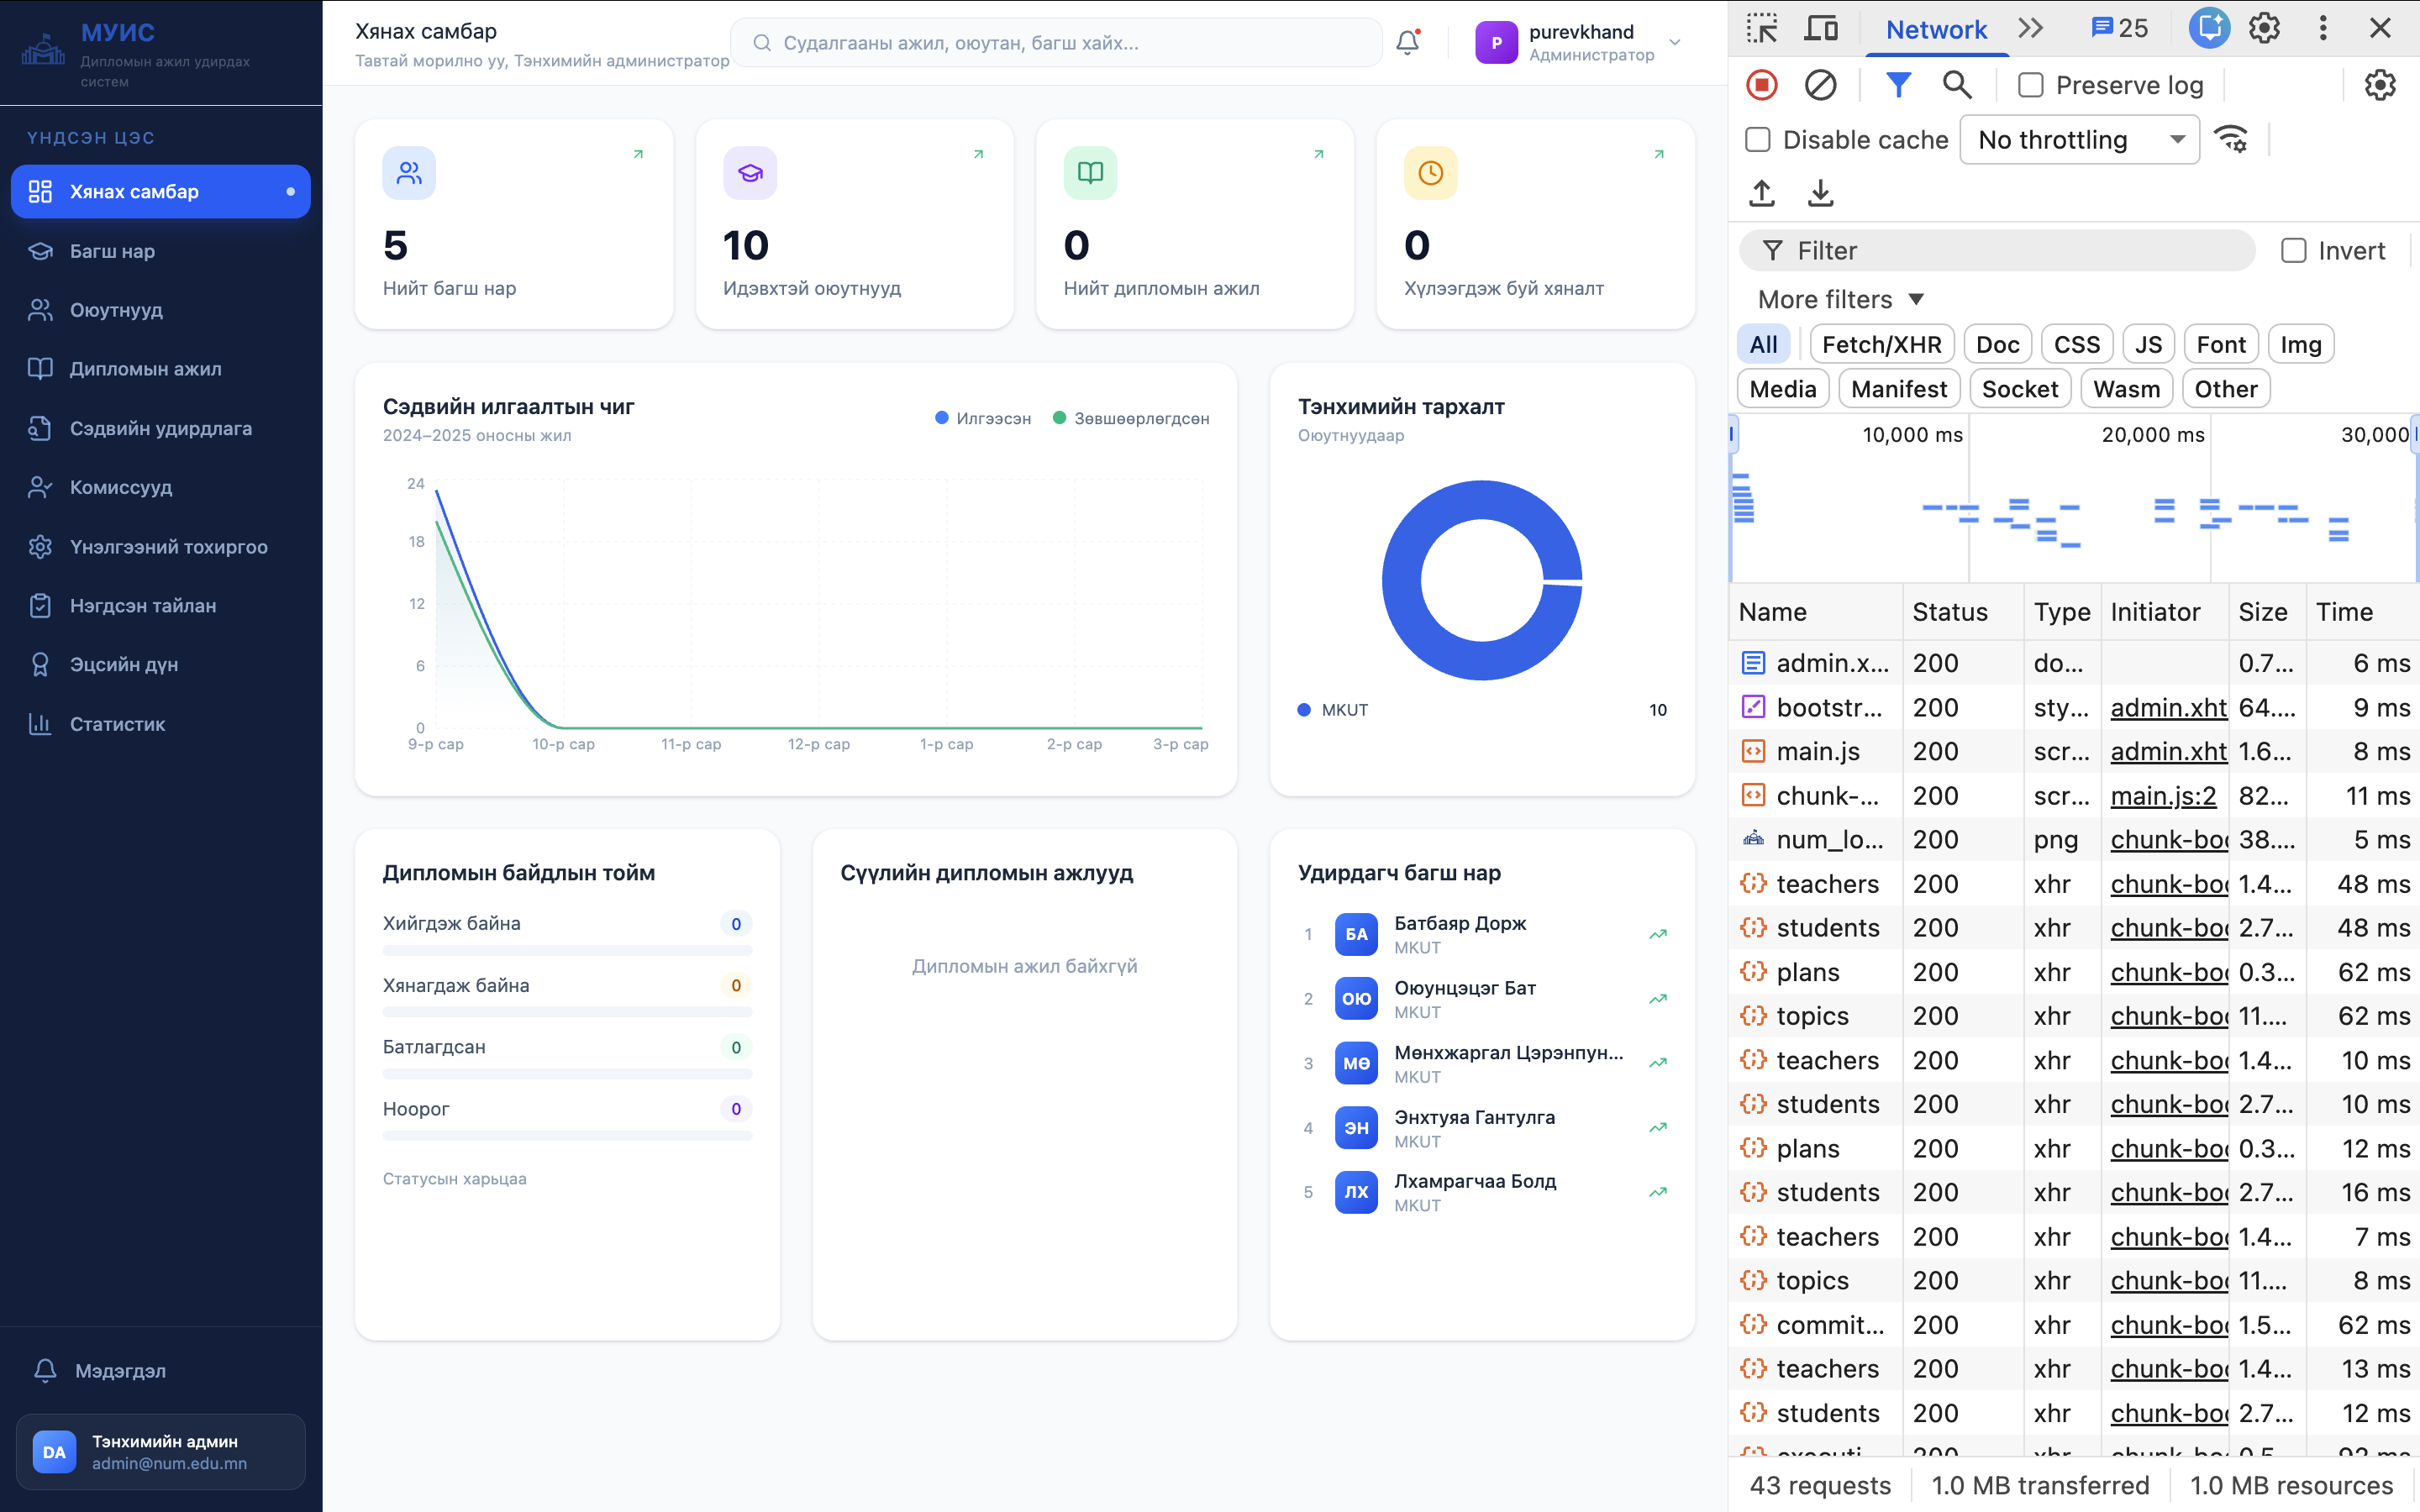
\includegraphics[width=14cm]{images/fig_implementation_summary.png}
    \caption{Зураг 4.10. Системийн хэрэгжүүлэлтийн нэгдсэн бүдүүвч. Frontend MFE давхарга, Tomcat хост, backend микросервис, PostgreSQL өгөгдлийн давхарга нь нэгдсэн байдлаар хамтарч ажилладаг бүрэн дүр зургийг харуулна. Эх сурвалж: зохиогчийн судалгаа, 2026.}
    \label{fig:impl_summary}
\end{figure}
 гэж үндсэн файлд оруулна
% Шаардлагатай package-ууд: booktabs, float, graphicx, listings,
%   tabularx, amsmath, hyperref
% =====================================================================

3-р бүлэгт тодорхойлсон архитектурын загвар нь хийсвэр зарчмуудын
цуглуулга~--- энэхүү бүлэгт эдгээр зарчмуудыг бодит кодын дэс дараа,
тохиргооны файл, алдааны дүн шинжилгээ, инженерчлэлийн практик
шийдлийн хэлбэрт хувиргасан ажлыг баримтжуулна. Загварын ``юу'' нь
хэрэгжүүлэлтийн ``хэрхэн'' болж хувирах явцад тулгарсан техникийн
хүндрэл, нарийн шийдвэр, хийсвэрлэлийн тохируулгуудыг тайлбарлана.

% ─────────────────────────────────────────────────────────────────────
\section{Frontend Хэрэгжүүлэлт ба Нэгтгэлт}
% ─────────────────────────────────────────────────────────────────────

\subsection{Vite Module Federation-ийн Тохиргоо}

3-р бүлэгт Runtime Integration стратегийг сонгосны практик хэрэгжүүлэлт нь
\texttt{@originjs/vite-plugin-federation} хэрэгсэлд тулгуурласан. Уг
хэрэгсэл нь Webpack~5-ийн \texttt{ModuleFederationPlugin}-ийн Vite орчинд
ажилладаг хувилбар бөгөөд \texttt{remoteEntry.js} файл үүсгэж, Remote
MFE-ийн экспортлосон бүрэлдэхүүнүүдийг Host-д ачаалах боломжийг хангана.

MFE модуль тус бүрийн \texttt{vite.config.ts} нь дараах бүтэцтэй тохиргоог
дагана. \texttt{module-thesis} модулийн тохиргоо нь дараах байдалтай:

\begin{figure}[H]
    \centering
    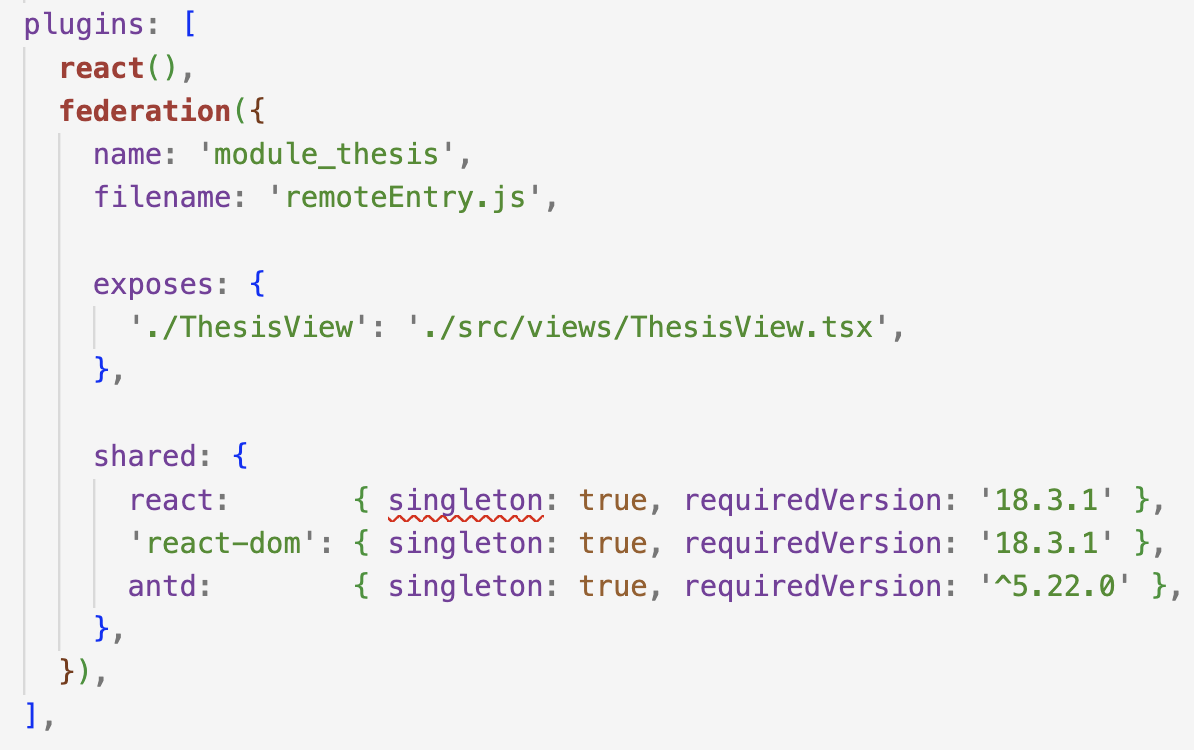
\includegraphics[width=14cm]{images/fig_vite_federation_config.png}
    \caption{Зураг 4.1. \texttt{module-thesis}-ийн \texttt{vite.config.ts} тохиргооны бүтэц. \texttt{name}, \texttt{filename}, \texttt{exposes}, \texttt{shared} дөрвөн гол тохиргооны цэгийг харуулна.}
    \label{fig:vite_config}
\end{figure}

Тохиргооны дөрвөн тулгуур параметрийг тайлбарлая:

\textbf{\texttt{name: 'module\_thesis'}:} Federation-ийн глобал нэрийн
орон зай (namespace). Browser-ийн \texttt{window} объект дээр энэ нэрийн
дор модулийн бүртгэл хийгдэнэ. Нэрийн зөрчлөөс зайлсхийхийн тулд
дор хаяж нэг давхарга нэртэй prefix ашиглах зарчмыг дагав.

\textbf{\texttt{filename: 'remoteEntry.js'}:} Remote MFE-ийн ``агуулгын
хүснэгт'' болох файлын нэр. Host нь энэ URL-г динамикаар \texttt{<script>}
tag хэлбэрт DOM-д оруулах замаар Remote-ийн бүртгэлийг ачаалдаг.

\textbf{\texttt{exposes: \{ './ThesisView': '...' \}}:} Энэ Remote-аас
Host-д нээлттэй байх бүрэлдэхүүнүүд. Дан \texttt{'./ThesisView'} экспортлосон
нь нэгдсэн зарчмыг баримтлж байна~--- нэг Remote нь нэг бизнесийн чадвар.

\textbf{\texttt{shared: \{ react, 'react-dom', antd \}}:} Singleton
хэлбэрт хуваалцагдах хамаарлууд. \texttt{singleton: true} тохиргоо нь
Host болон бүх Remote нэг React instance ашиглахыг баталгаажуулна~---
ингэснээр \texttt{useState}, \texttt{useContext} hook-ууд хөндлөн модулийн
хооронд зөв ажиллана.

\subsection{Runtime Integration: JSF-ийн Script Injection Механизм}

JSF хостын хуудсанд React MFE-г ачаалах гол механизм нь динамик
\texttt{<script>} tag injection юм. Production орчинд Tomcat~8080-д
\texttt{/microfrontends/} замаар static файлуудыг хүргэдэг бол
development орчинд \texttt{http://localhost:30XX} хаягаар Vite-ийн
dev server ажилладаг.

JSF-ийн \texttt{.xhtml} хуудсанд MFE-г ачаалах хэсэг нь дараах
ерөнхий бүтэцтэй:

\begin{figure}[H]
    \centering
    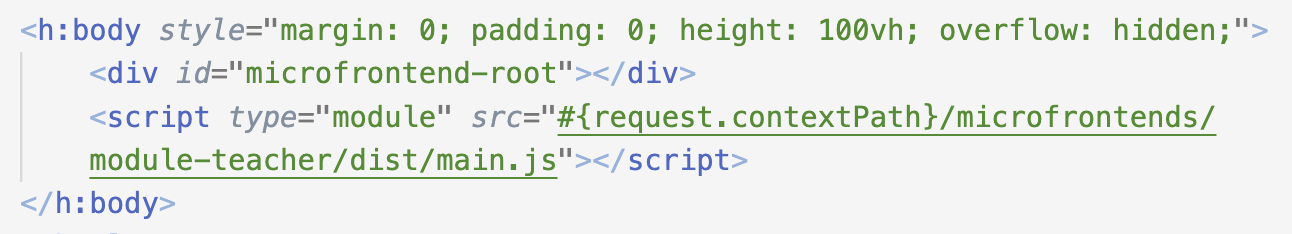
\includegraphics[width=14cm]{images/fig_jsf_script_injection.png}
    \caption{JSF \texttt{.xhtml} хуудасны MFE injection механизм. \texttt{remoteEntry.js} ачаалагдсаны дараа bootstrap.js нь \texttt{<div id="microfrontend-root">} дотор React компонентийг render хийнэ}
    \label{fig:jsf_injection}
\end{figure}

Injection-ийн техникийн дэс дараа:

\begin{enumerate}
  \item JSF Facelets нь хуудсыг server-side render хийхдээ
    \texttt{<div id="microfrontend-root"/>} DOM цэгийг байрлуулна.
  \item \texttt{<script type="module" src=".../remoteEntry.js"/>} tag
    нь браузерт Remote Federation-ийн manifest-ийг ачаална.
  \item \texttt{<script type="module">} блок нь динамик \texttt{import()}
    ашиглан Remote-ийн экспортлосон компонентийг авна.
  \item React-ийн \texttt{createRoot(\#microfrontend-root).render(\ldots)}
    нь тухайн DOM цэгт компонентийг mount хийнэ.
  \item React Router-ийн \textbf{HashRouter} ашигладгийн шалтгаан нь
    JSF-ийн FacesServlet нь \texttt{/student/*} гэх URL pattern-ийг
    хариуцдаг бөгөөд React SPA маршрутлалт нь JSF-тэй зөрчилддгийг
    арилгахын тулд \texttt{/\#/student/dashboard} хэлбэрийн hash-based
    routing хэрэглэнэ.
\end{enumerate}

\subsection{Маршрутлалтын Хүндрэл ба HashRouter Шийдэл}

MFE архитектурт маршрутлалтын хоёр давхарга байдаг: нэгдүгээр давхарга
нь JSF хостын маршрутлалт (\texttt{FacesServlet}-ийн URL pattern), хоёрдугаар
давхарга нь тухайн MFE-ийн React Router дотоод маршрутлалт. Эдгээр хоёр
давхарга зөрчилдөхөд \textbf{``404 Not Found''} буюу JSF-ийн хуудас олдохгүй
алдаа гардаг.

Энэ зөрчлийг шийдвэрлэх хоёр арга байна:

\begin{enumerate}
  \item \textbf{HistoryRouter + Server Catch-all:} Tomcat-д
    \texttt{<url-pattern>/student/*</url-pattern>} бүгдийг нэг JSF
    хуудас руу шилжүүлж, React Router-ийн \texttt{createBrowserRouter}
    ашиглана. Тохиргоо нарийн боловч хэрэглэгчийн URL чухал.
  \item \textbf{HashRouter:} URL-ийн \texttt{\#} хэсэг нь сервер рүү
    хэзээ ч явдаггүй тул JSF-тэй зөрчилддөггүй. React Router-ийн
    \texttt{HashRouter} нь \texttt{/\#/thesis/list} хэлбэрийн URL
    ашиглан дотоод маршрутлалтыг зохицуулна.
\end{enumerate}

Энэ системд \texttt{HashRouter} сонгосны шалтгаан нь: JSF-ийн \texttt{web.xml}
болон \texttt{faces-config.xml}-ийн нарийн URL pattern тохиргоог өөрчлөх
нь монолитийн дотоод урсгалд нөлөөлнө гэсэн эрсдэлтэй байсан тул
хамгийн бага өөрчлөлтийн зарчмаар \texttt{HashRouter}-ийг сонгов.

\subsection{JWT болон Глобал Төлөвийн Хуваалцалт}

JSF хост болон React MFE хоорондын хэрэглэгчийн нэвтрэлтийн мэдлэгийн
хуваалцалт нь архитектурын хамгийн нарийн хэсэг юм. Хэрэглэгч
\texttt{module-auth}-д нэвтрэхэд дараах дараалал гүйцэтгэгдэнэ:

\begin{figure}[H]
    \centering
    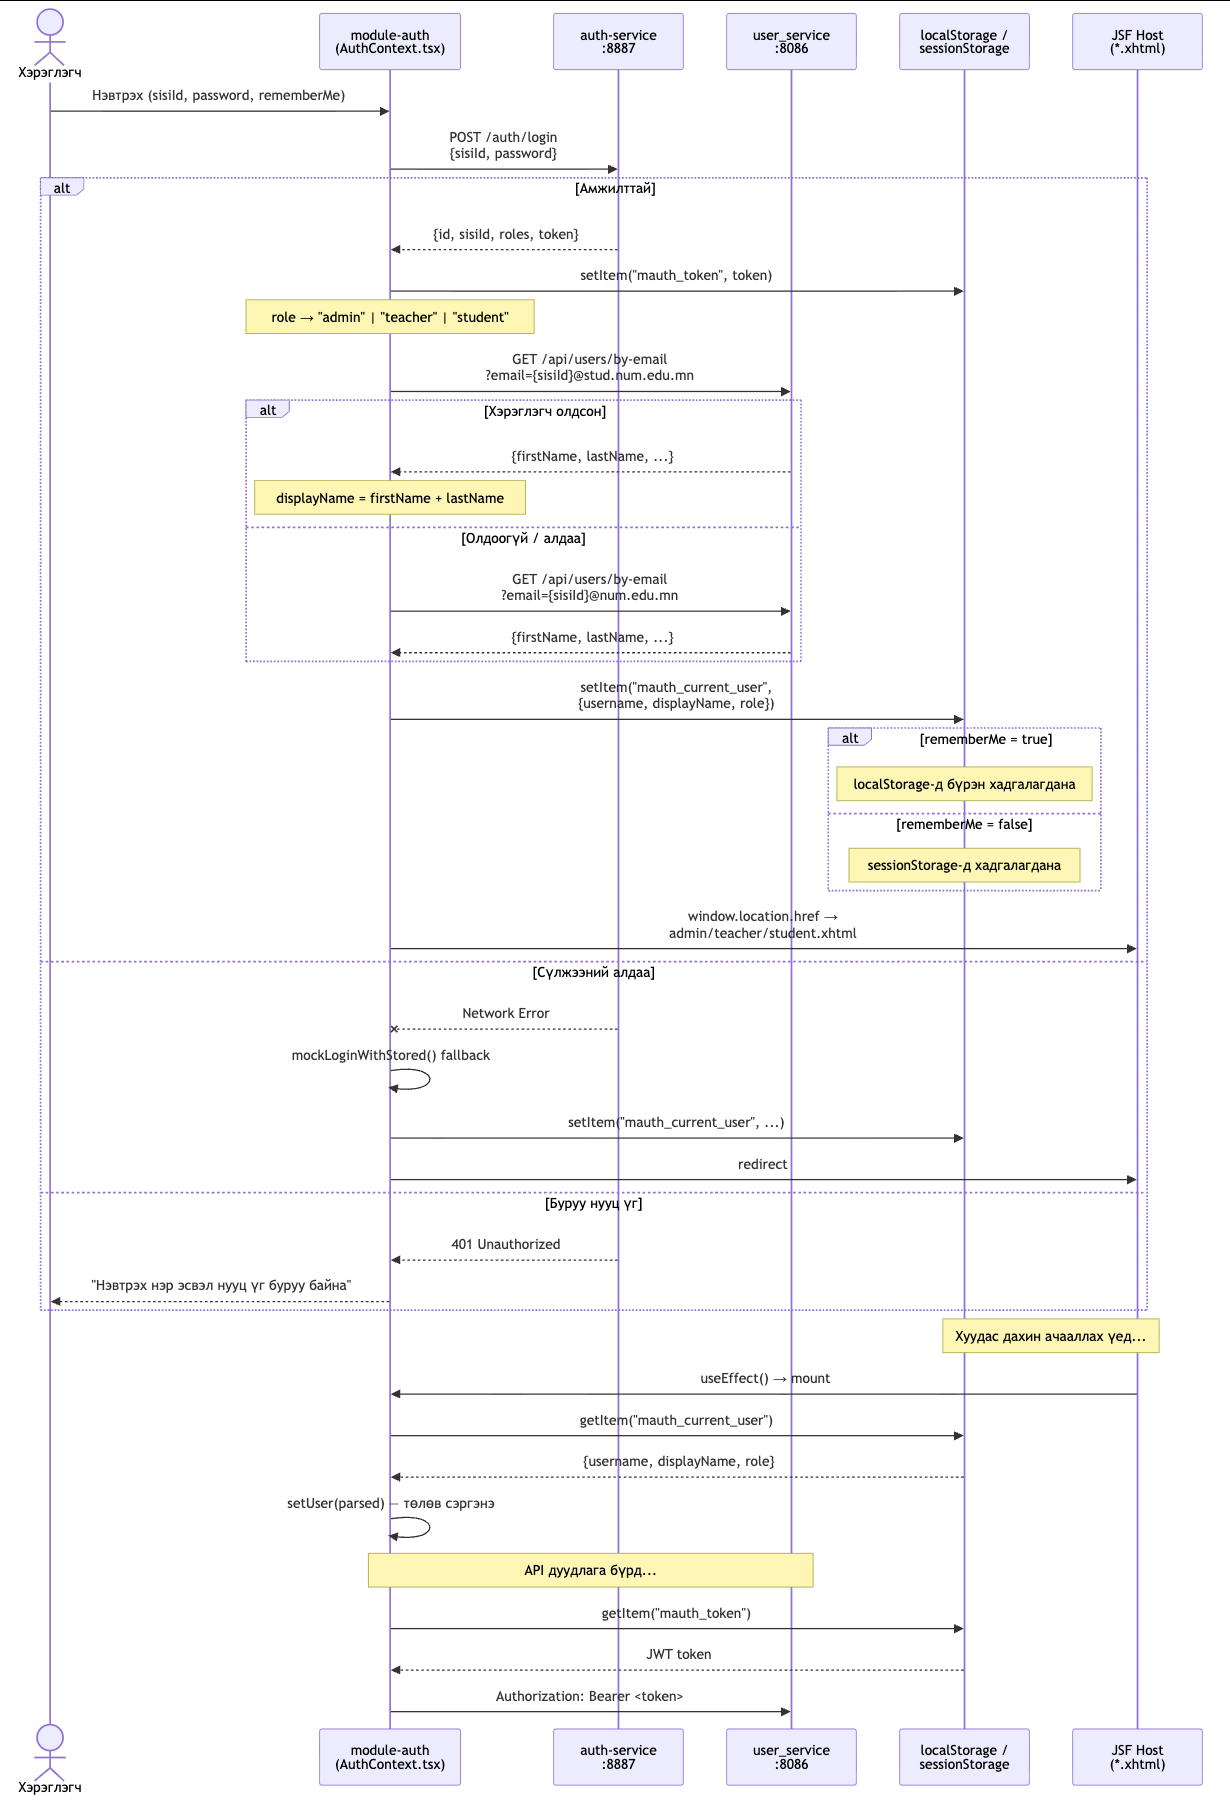
\includegraphics[width=14cm]{images/fig_jwt_flow_sequence.png}
    \caption{JWT нэвтрэлтийн дараалалт диаграм. Auth MFE нь токений хүсэлт илгээж, хүлээн авсан JWT-г localStorage-д хадгалах бөгөөд бусад MFE-ууд нь тэндээс JWT-г уншиж API дуудлагад ашиглана}
    \label{fig:jwt_flow}
\end{figure}

Хуваалцах механизм нь \texttt{localStorage} дотор тодорхой key-д JSON
объект хэлбэрт хадгалагдана:

\begin{itemize}
  \item \texttt{mauth\_token}: JWT Bearer токен~--- API дуудлага бүрийн
    \texttt{Authorization: Bearer \ldots} header-т ашиглагдана.
  \item \texttt{mauth\_current\_user}: \texttt{\{username, displayName,
    role\}} бүтэцтэй JSON~--- хэрэглэгчийн нэр, дүр зэргийг хадгалана.
\end{itemize}

Дизайн шийдвэрийн үндэслэл: \texttt{localStorage} нь хуудас дахин
ачааллагдах (page refresh) болон хэд хэдэн browser tab хооронд бүтэн
хадгалагддаг. \texttt{sessionStorage} нь tab хаагдахад устдаг тул
``Намайг санах'' (Remember Me) функцийг дэмжихгүй. Аюулгүй байдлын
хувьд \texttt{HttpOnly Cookie} нь XSS халдлагаас хамгаалалт сайн боловч
JSF-ийн хуудасны дагуу cookie scope нарийн удирдлага шаардана~---
тул энэ прототипд \texttt{localStorage} ашигласан бөгөөд үйлдвэрлэлийн
орчинд \texttt{HttpOnly} cookie руу шилжихийг зөвлөмж болгоно.

\texttt{AuthContext.tsx} нь React-ийн Context API-д суурилсан global
state provider бөгөөд MFE модуль бүрийн root-д байрладаг. Хуудас
ачааллагдах бүрт localStorage-ийн утгыг уншиж, хэрэглэгчийн төлөвийг
сэргээдэг. Нэвтрэлтийн дараалал нь дараах байна: эхлээд
\texttt{POST http://localhost:8887/auth/login} руу \texttt{\{sisiId,
password\}} илгээнэ; амжилттай тохиолдолд хариуд JWT токен болон
дүрийн мэдээлэл ирнэ; дараа нь \texttt{GET http://localhost:8086/api/users/by-email}
руу хүсэлт илгээж хэрэглэгчийн дэлгэрэнгүй нэрийг авна; эцэст нь
дүрд тохирсон URL руу чиглүүлнэ.

\subsection{Shared-UI ба Singleton Хамаарлын Зохицуулалт}

3-р бүлэгт тодорхойлсон \texttt{shared-ui} модуль нь практик хэрэгжүүлэлтэд
нарийн техникийн хүндрэлтэй тулгарав. Анх nested federation загвараар~---
\texttt{module-thesis} нь \texttt{shared\_ui} Remote-ийг агуулах~---
загварчилсан боловч хэрэгжүүлэлтийн явцад критик алдаа илэрлээ:

\texttt{TypeError: Failed to resolve module specifier '\$\{\_\_federation\_expose\_./SharedUI\}'}

Энэ алдааны үндэс нь \texttt{@originjs/vite-plugin-federation} нь
Remote-ийн \texttt{remoteEntry.js}-д Remote-ийн Remote-ийн URL template-ийг
динамикаар тохируулах механизм дутмаг байдаг явдал юм. Tomcat-д статик
файл хэлбэрт хүргэгдсэн Remote нь өөрийн nested Remote-ийн URL-г
тодорхойлж чадахгүй.

\textbf{Шийдэл:} Nested federation-ийн оронд \texttt{shared-ui}-ийн
бүрэлдэхүүнүүдийг (\texttt{PageHeader}, \texttt{PortalTabs},
\texttt{StatusBadge}, \texttt{DataTable}) тухайн Remote-ийн дотор шууд
нэгтгэж, Ant Design-ийг federation-ийн \texttt{shared singleton}
механизмаар хуваалцана. Энэ нь кодын хуулбарлалтын зардалтай боловч
runtime-д нэг antd instance ашиглагддаг тул bundle хэмжээ нэмэгдэхгүй.

\begin{figure}[H]
    \centering
    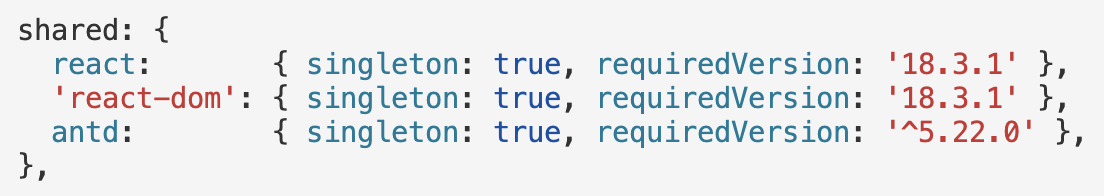
\includegraphics[width=14cm]{images/fig_shared_singleton_pattern.png}
    \caption{Shared Singleton загварын зохицуулалт. Antd нь нэгдсэн singleton хэлбэрт ачааллагдаж, Remote модуль бүр энэ нэг instance-ийг ашиглана~--- nested federation-ийн алдааг арилгана. Эх сурвалж: зохиогчийн судалгаа, 2026.}
    \label{fig:shared_singleton}
\end{figure}

\subsection{Build ба Deploy Паплайн}

Хэрэгжүүлэлтийн орчинд \texttt{build-modules.sh} shell скрипт нь
бүх MFE модулийг дараалан build хийж, \texttt{dist/} гаралтыг
Tomcat-ийн \texttt{webapps/microfrontends/\{module-name\}/dist/}
хавтаст хуулдаг. Скриптийн ерөнхий урсгал нь:

\begin{enumerate}
  \item MFE модуль бүрийн \texttt{npm run build} ажиллуулна.
  \item \texttt{dist/assets/remoteEntry.js} файлыг \texttt{dist/}
    root рүү хуулна~--- \texttt{@originjs}-ийн хуучин хувилбар нь
    \texttt{remoteEntry.js}-г \texttt{dist/assets/} дотор үүсгэдэг
    тул Host-ийн URL тохиргоотой зөрчилддгийг засна.
  \item Томкат нь \texttt{/microfrontends/\{module\}/dist/remoteEntry.js}
    замаар тухайн Remote-ийн manifest-ийг хүргэнэ.
\end{enumerate}

\begin{figure}[H]
    \centering
    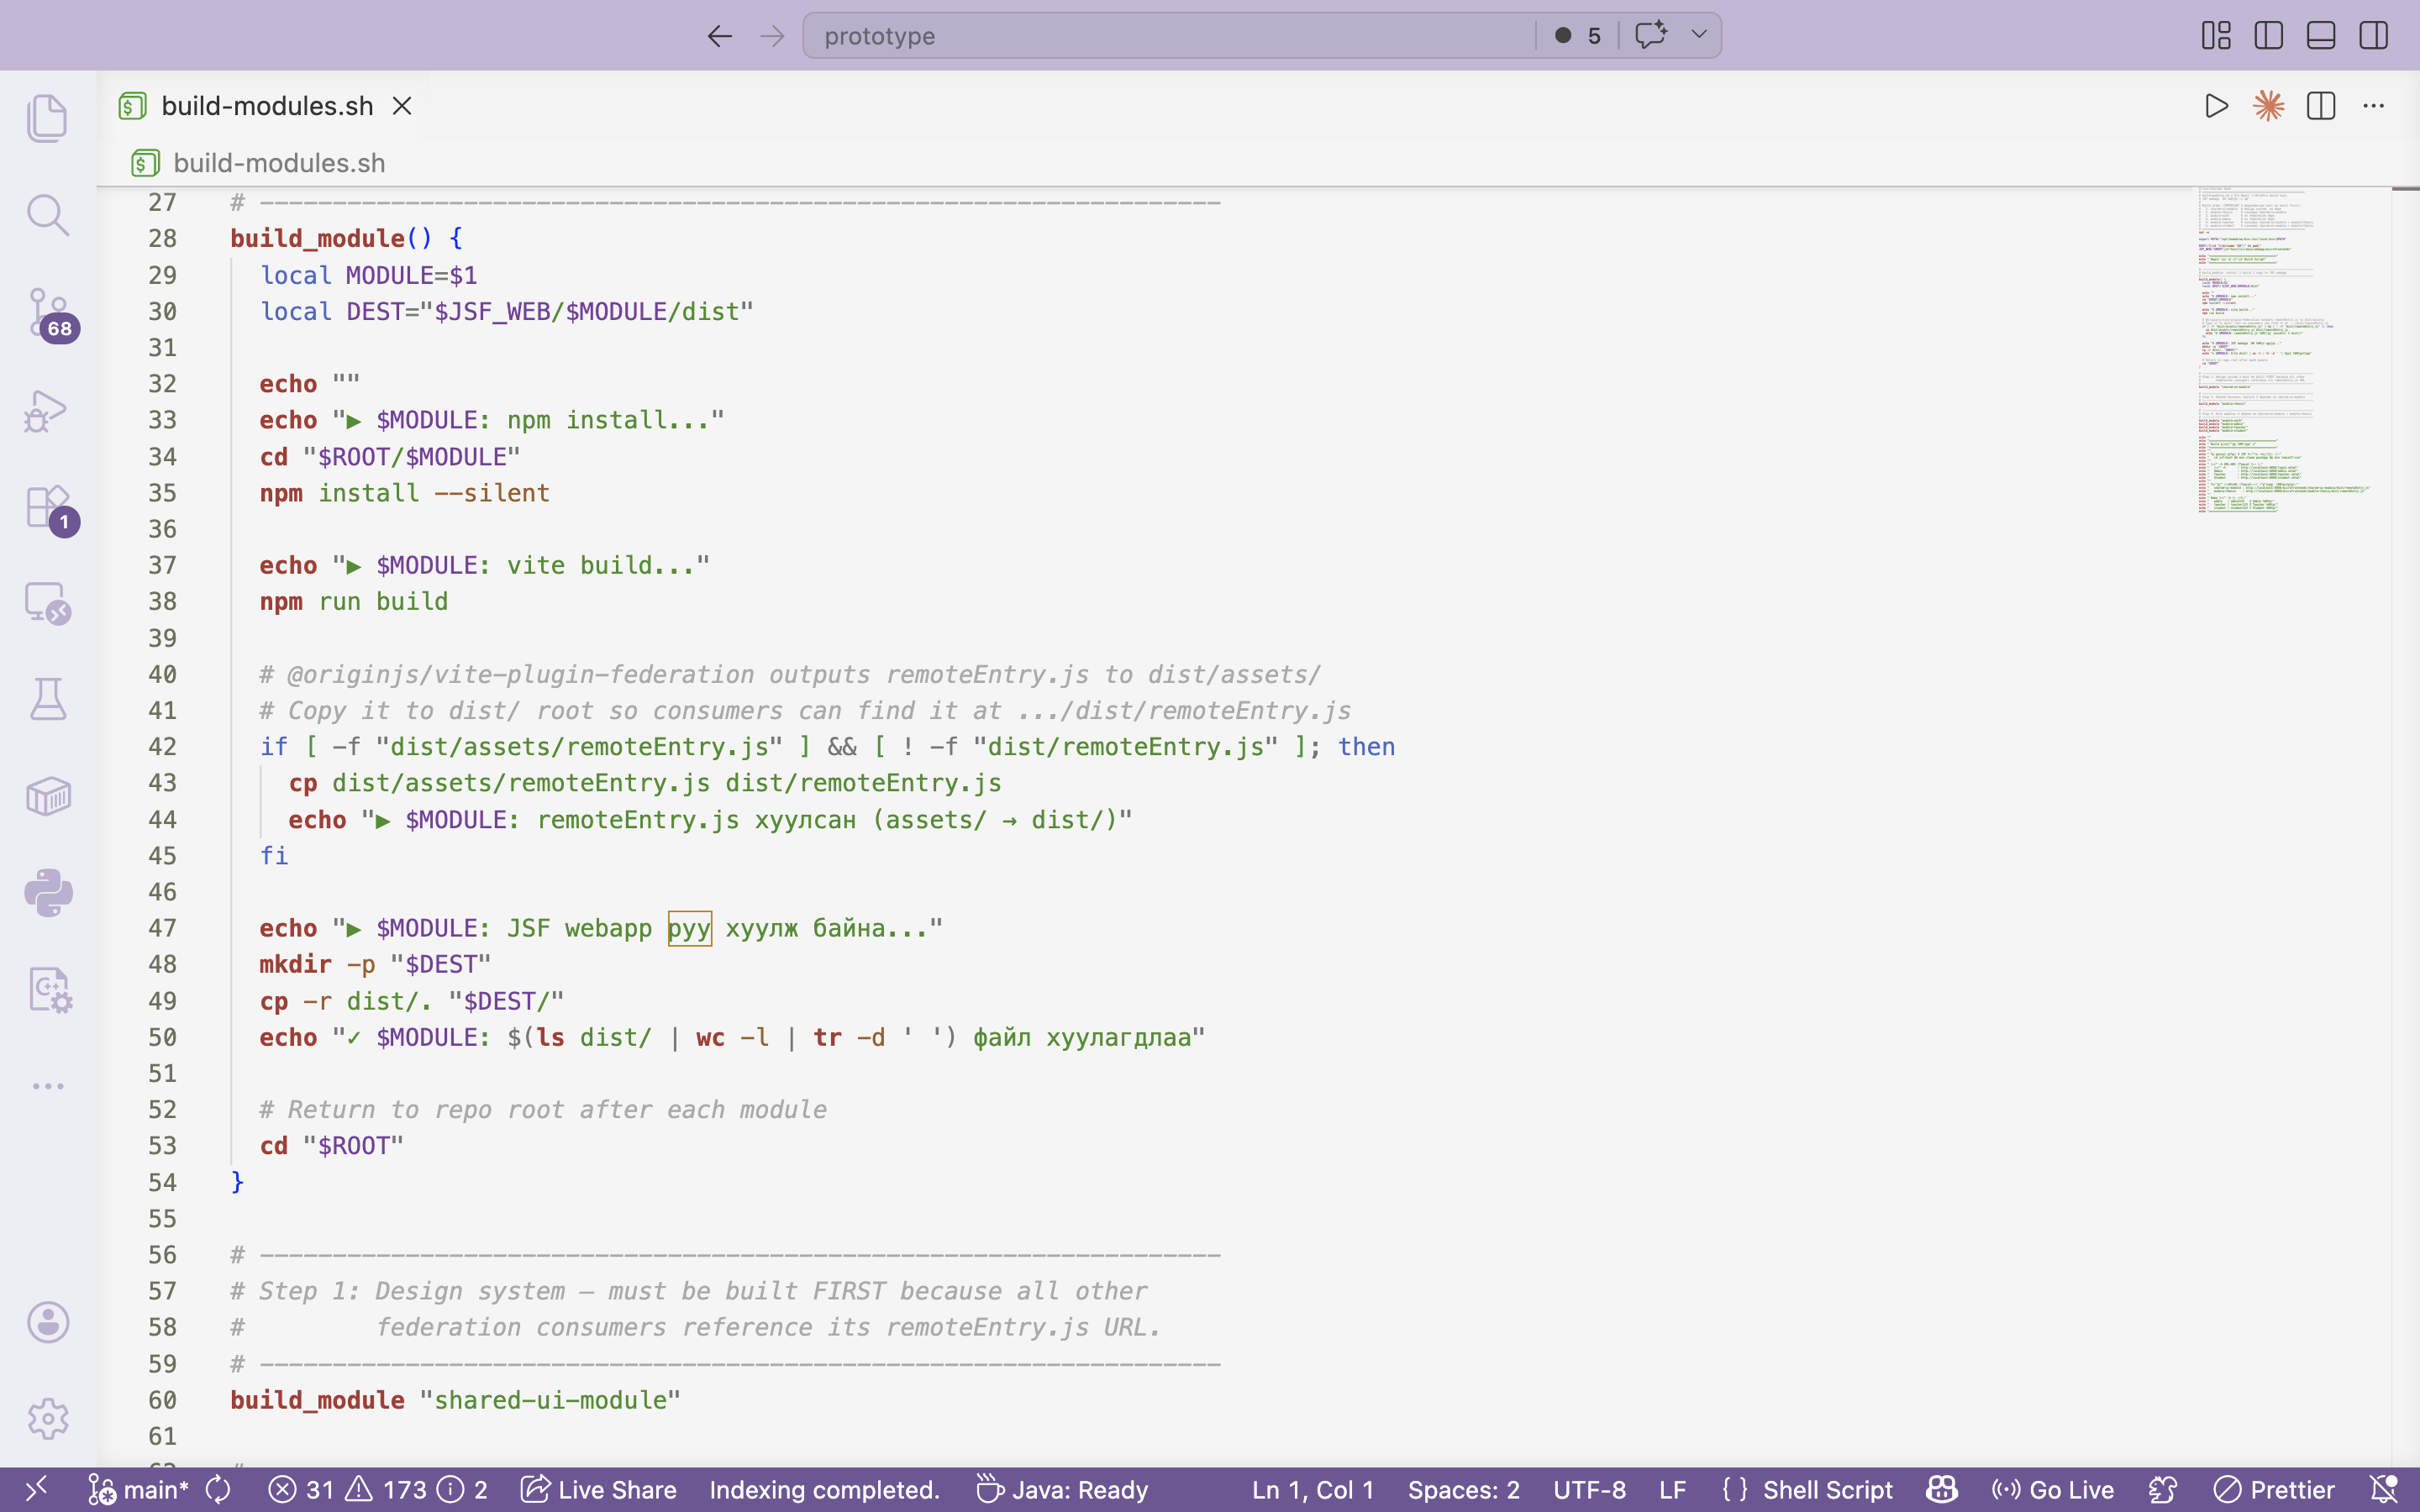
\includegraphics[width=14cm]{images/fig_build_deploy_pipeline.png}
    \caption{Зураг 4.5. Build ба Deploy паплайны урсгалын диаграм. Модуль тус бүрийн Vite build гаралт нь Tomcat-ийн webapps хавтасрт хуулагдаж, нэгдсэн байдлаар 8080 порт дээр хүргэгдэнэ. Эх сурвалж: зохиогчийн судалгаа, 2026.}
    \label{fig:build_pipeline}
\end{figure}

% ─────────────────────────────────────────────────────────────────────
\section{Backend Хэрэгжүүлэлт}
% ─────────────────────────────────────────────────────────────────────

\subsection{Spring Boot болон Spring WebFlux-ийн Сонголт}

Backend микросервисүүдийн хэрэгжүүлэлтэд Java~21 болон Spring Boot~3.2.x
framework-ийг ашиглав. Гэвч 3-р бүлгийн 3.3.2-т тодорхойлсон масштабдах
чадварын шаардлагын дагуу уламжлалт \textbf{Spring MVC} (thread-per-request)
загварын оронд \textbf{Spring WebFlux} (reactive, event-loop) загварыг
сонгов.

Spring MVC нь request бүрт нэг thread хуваарилдаг тул 1,000 зэрэгцэх
хүсэлт нь 1,000 thread шаарддаг~--- JVM-ийн thread stack дундажаар 512~КБ
тул 1,000 thread нь $\approx$~500~МБ санах ой хэрэглэнэ. Spring WebFlux
нь Netty-ийн Non-blocking I/O event-loop дээр суурилж, CPU-ийн цөмийн
тоо ($n$) thread-аар хэдэн мянган зэрэгцэх холболтыг удирддаг.

\textbf{Hexagonal Architecture (Ports and Adapters):} Сервис тус бүрийн
дотоод бүтэц нь Alistair Cockburn (2005)-ийн Hexagonal Architecture
зарчмаар зохион байгуулагдсан:

\begin{itemize}
  \item \textbf{Domain Layer:} Бизнесийн логик агуулсан цөм~---
    жишээ нь \texttt{Thesis}, \texttt{WorkflowState} домейн объектууд.
    Аль ч фреймворкоос тусгаарлагдсан цэвэр Java/Kotlin класс.
  \item \textbf{Application Layer (Ports):} Use Case интерфэйс~---
    \texttt{CreateStudentUseCase}, \texttt{FindUserUseCase},
    \texttt{SubmitThesisUseCase}. Домейн логикийг хэрхэн дуудах
    гэрээг тодорхойлно.
  \item \textbf{Adapter Layer:} Гадаад ертөнцтэй холбогч~---
    \texttt{UserController} (HTTP adapter), \texttt{UserR2dbcRepository}
    (persistence adapter), \texttt{NotificationWebSocketAdapter}
    (messaging adapter).
\end{itemize}

\begin{figure}[H]
    \centering
    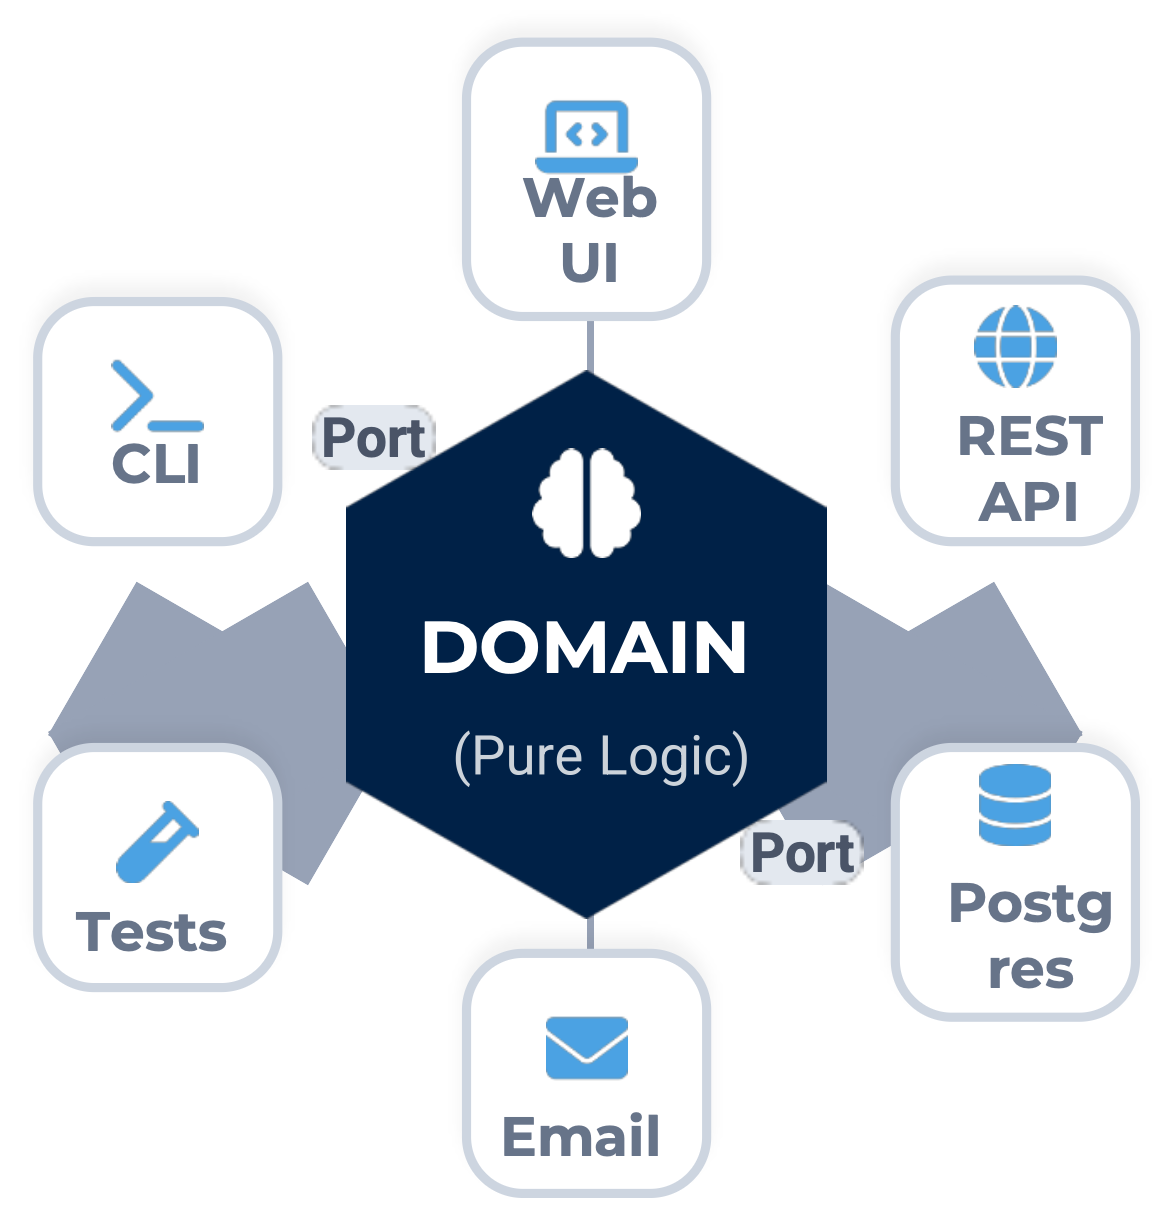
\includegraphics[width=14cm]{images/fig_hexagonal_architecture.png}
    \caption{Hexagonal Architecture-ийн \texttt{user\_service} дахь хэрэгжүүлэлтийн бүтэц. Домейн давхарга нь дотор цагирагт, Port-ууд нь дунд цагирагт, Adapter-ууд нь гадаад цагирагт байрлана. Эх сурвалж: зохиогчийн судалгаа, 2026.}
    \label{fig:hexagonal_arch}
\end{figure}

\subsection{Микросервис Тус Бүрийн Хэрэгжүүлэлтийн Нарийн}

\subsubsection{auth-service ба JWT Токений Хэрэгжүүлэлт}

\texttt{auth-service} нь \texttt{sisiId} болон нууц үг хүлээн авч, хэрэглэгчийн
бичлэгтэй харьцуулж, \texttt{jjwt}~(Java JWT) санг ашиглан токен
үүсгэнэ. Токений payload нь \texttt{\{sub: sisiId, roles: [...],
iat: epochSeconds, exp: iat+86400\}} бүтэцтэй. Нийтийн болон хувийн
түлхүүрийн хос (RSA-256)-ийн оронд энэ прототипд HMAC-SHA256 алгоритмтай
нийтлэг нууц key ашиглагдав~--- үйлдвэрлэлийн орчинд RSA key pair
болон Key Management Service (KMS) ашиглахыг зөвлөмж болгоно.

\texttt{authorization-service} нь дүр болон эрхийн матрицийг удирдана.
\texttt{ROLE\_ADMIN}, \texttt{ROLE\_TEACHER}, \texttt{ROLE\_STUDENT},
\texttt{ROLE\_COMMITTEE\_MEMBER} дүрүүд тодорхойлогдсон бөгөөд endpoint
бүр дээр Spring Security-ийн \texttt{@PreAuthorize} annotationоор
хандах эрхийн шалгалт хэрэгжинэ.

\subsubsection{user\_service-ийн Reactive Хэрэгжүүлэлт}

\texttt{user\_service} нь Spring WebFlux болон R2DBC-г хослуулан ашиглах
бөгөөд \texttt{UserController}-д хэрэглэгчийн CRUD болон хайлтын
endpoint-ууд хэрэгждэнэ. \texttt{/api/users/by-email} endpoint нь
\texttt{UserR2dbcRepository.findByEmail(String email)} reactive метод
дуудаж, \texttt{Mono<User>} буцаана~--- энэ нь AuthContext-ийн
display name lookup-д зориулан нэмэгдсэн.

\texttt{UserR2dbcRepository} нь \texttt{ReactiveCrudRepository<User, String>}
интерфэйсийг өргөтгөсөн бөгөөд Spring Data R2DBC нь SQL query-г
\texttt{findBy\{FieldName\}} нэрлэлтийн конвенцоос автоматаар үүсгэнэ.
Энэ нь ``конвенц дагасан тохиргоо'' (convention over configuration)
зарчмын практик хэрэглэлт бөгөөд boilerplate кодын хэмжээг мэдэгдэхүйц
бууруулна.

\subsubsection{workflow\_service-ийн State Machine Хэрэгжүүлэлт}

\texttt{workflow\_service} нь дипломын ажлын статус шилжилтийг хариуцна.
State Machine нь Java-ийн enum болон явцын хамгаалагдсан шилжилтийн
матрицаар хэрэгжинэ:

\begin{table}[H]
    \centering
    \caption{Дипломын ажлын статус шилжилтийн зөвшөөрөгдсөн матриц}
    \label{tab:workflow_transitions}
    \renewcommand{\arraystretch}{0.7}
    \begin{tabular}{lll}
        \toprule
        \textbf{Одоогийн статус} & \textbf{Зорилтот статус} & \textbf{Хэн гүйцэтгэх} \\
        \midrule
        DRAFT              & SUBMITTED           & Оюутан \\
        SUBMITTED          & UNDER\_REVIEW       & Удирдагч багш \\
        SUBMITTED          & REJECTED            & Удирдагч багш \\
        UNDER\_REVIEW      & REVISION\_REQUESTED & Удирдагч багш \\
        UNDER\_REVIEW      & APPROVED            & Удирдагч багш \\
        REVISION\_REQUESTED & SUBMITTED          & Оюутан \\
        APPROVED           & DEFENSE\_SCHEDULED  & Систем / Админ \\
        DEFENSE\_SCHEDULED & DEFENDED            & Хорооны гишүүн \\
        DEFENDED           & ARCHIVED            & Систем \\
        \bottomrule
    \end{tabular}
\end{table}

Зөвшөөрөгдөөгүй шилжилтийн оролдлого нь \texttt{HTTP 422 Unprocessable
Entity} буцаах бөгөөд хариу body нь шилжилт яагаад зөвшөөрөгдөхгүй
байгаа шалтгааны тайлбарыг агуулна.

\subsection{API Gateway-ийн Тохиргоо}

Тус системд тусдаа API Gateway сервис биш харин \textbf{Tomcat-ийн
reverse proxy} тохиргоо gateway-ийн үүрэг гүйцэтгэнэ. Apache Tomcat
нь \texttt{server.xml}-д \texttt{ProxyPass} директивоор (эсвэл Nginx
reverse proxy хослуулан) backend сервисүүд рүү HTTP хүсэлтийг
чиглүүлнэ. Энэ нь Nginx эсвэл Spring Cloud Gateway-тай харьцуулахад
хялбар боловч илүү нарийн CORS, rate limiting, circuit breaker
хяналт шаарддаг тул ирээдүйн шатанд тусдаа gateway нэвтрүүлэх
хэрэгцээ байна.

Frontend JavaScript-аас API дуудлагын CORS тохиргоо нь сервис
бүрийн \texttt{application.yml}-д тохируулагдсан:

\begin{figure}[H]
    \centering
    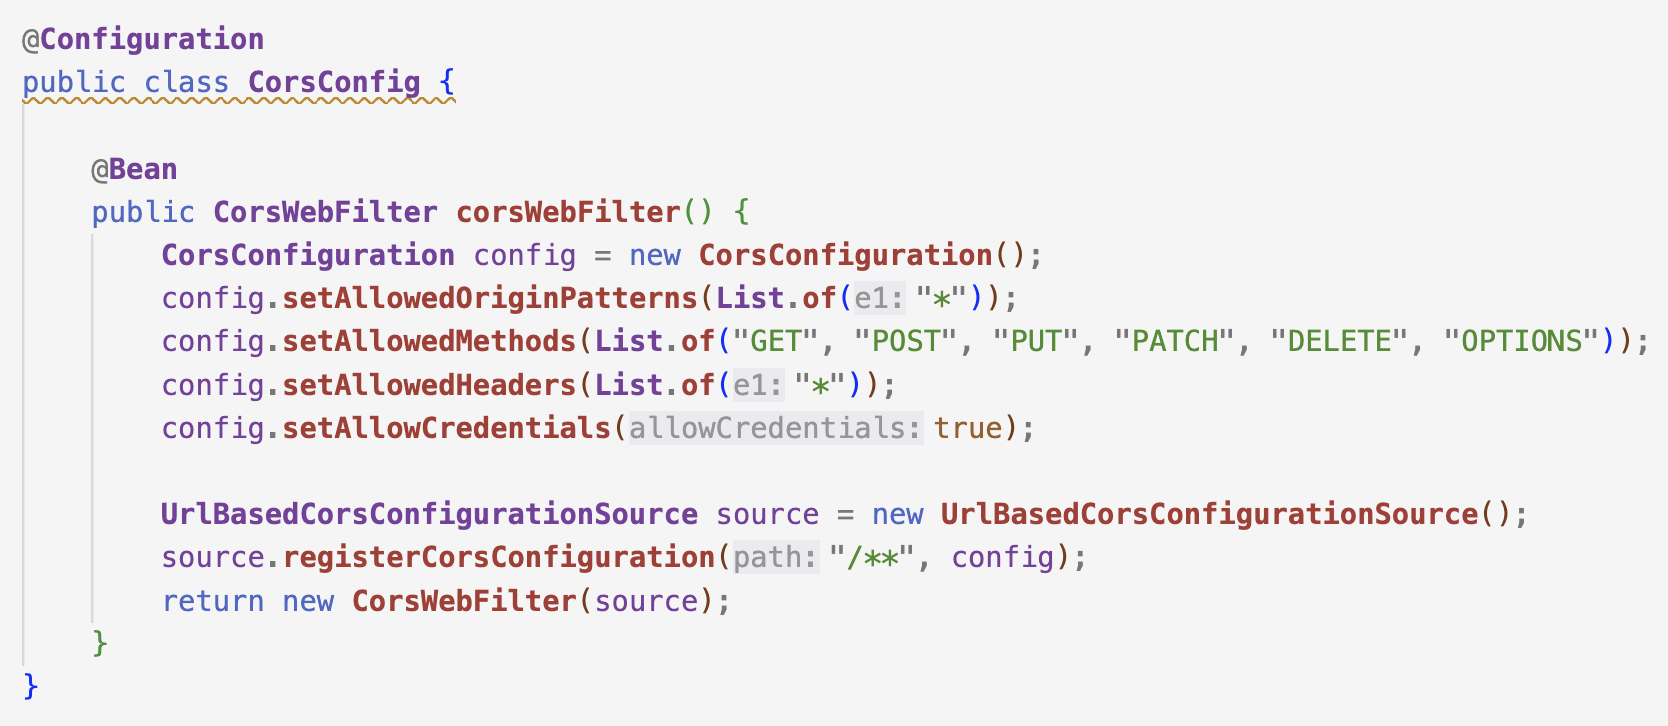
\includegraphics[width=14cm]{images/fig_cors_config.png}
    \caption{Зураг 4.7. Spring WebFlux-ийн CORS тохиргооны жишээ. \texttt{allowedOrigins} нь Tomcat-ийн 8080 порт, \texttt{allowedMethods} нь REST стандартын бүх method-уудыг агуулна. Эх сурвалж: зохиогчийн судалгаа, 2026.}
    \label{fig:cors_config}
\end{figure}

\texttt{allowedOrigins: "http://localhost:8080"} нь зөвхөн JSF хостын
хаягаас ирсэн AJAX хүсэлтийг зөвшөөрнө. Үйлдвэрлэлийн орчинд
энэ нь бодит domain нэрийг агуулна, wildcard (\texttt{*}) ашиглахаас
зайлсхийнэ.

\subsection{Distributed Tracing-ийн Хэрэгжүүлэлт}

Сервисүүдийн хоорондох хүсэлтийн урсгалыг хянах Distributed Tracing-ийг
OpenTelemetry Java Agent болон Jaeger-ийн хослолоор хэрэгжүүлэв.
JVM startup parameter-т \texttt{-javaagent:opentelemetry-agent.jar}
нэмснээр application кодыг өөрчлөхгүйгээр HTTP request бүрт
\texttt{traceparent}, \texttt{tracestate} W3C стандартын trace header
автоматаар нэмэгдэнэ.

Нэг хэрэглэгчийн хүсэлт хэд хэдэн сервисийг дамжих бүрт нэг
\texttt{traceId}-ийн дор бүх span-ууд нэгтгэгдэнэ~--- Jaeger UI-д
waterfall диаграм хэлбэрт харагддаг бөгөөд сервис бүрийн саатал
(latency contribution) тус тусад нь хэмжигдэнэ. Оюутан дипломын ажил
илгээхэд \texttt{POST /api/thesis/submit}-ийн trace нь
\texttt{auth-service} (JWT шалгах), \texttt{thesis-service}
(бичлэг шинэчлэх), \texttt{workflow-service} (статус шилжүүлэх),
\texttt{notification-service} (мэдэгдэл илгээх) гэсэн 4 span агуулдаг.

% ─────────────────────────────────────────────────────────────────────
\section{Өгөгдлийн Сангийн Хэрэгжүүлэлт}
% ─────────────────────────────────────────────────────────────────────

\subsection{PostgreSQL болон R2DBC-ийн Сонголт}

3-р бүлгийн өгөгдлийн давхаргын загварчлалд PostgreSQL-г харилцааны
(relational) өгөгдлийн санаар, R2DBC-г реактив driver хэлбэрт сонгосон
байсан. Практик хэрэгжүүлэлтэд PostgreSQL~16.2 болон
\texttt{io.r2dbc:r2dbc-postgresql:1.0.4} driver ашиглав.

\textbf{Яагаад PostgreSQL:} Дипломын ажлын бизнесийн логик нь олон
харилцаатай өгөгдлийн бүтэц (User $\leftrightarrow$ Thesis
$\leftrightarrow$ Committee $\leftrightarrow$ Evaluation) агуулдаг
тул харилцааны бүрэн бүтэн байдлын баталгаа (referential integrity),
ACID transaction, SQL-ийн хүчирхэг query боломж шаардагдана. Document
store (MongoDB) нь schema-flexible боловч JOIN-ийн хэрэгцээтэй энэ
домейнд неудобен.

\textbf{Яагаад R2DBC (JDBC биш):} Spring WebFlux-ийн event-loop
загвар нь blocking JDBC дуудлагатай ``reactive pollution'' (цуваа
блоклолт) асуудалд орно~--- blocking call нь event-loop thread-ийг
хааж, бусад хүсэлтийн хариулт удаашралд орно. R2DBC нь Non-blocking
reactive driver тул WebFlux-тэй зохистой хэрэгждэнэ.

\subsection{Schema Тодорхойлолт ба Migration}

Сервис тус бүрийн өгөгдлийн сангийн schema нь тухайн сервисийн
\texttt{src/main/resources/schema\_\{service\_name\}.sql} файлд
тодорхойлогдсон. Эхний нэвтрэлтэд Spring Boot-ийн
\texttt{spring.sql.init.mode: always} тохиргоог ашиглан schema
автоматаар үүснэ. Үйлдвэрлэлийн орчинд Flyway эсвэл Liquibase
migration хэрэгслийг ашиглахыг зөвлөмж болгоно.

\texttt{user\_service}-ийн \texttt{schema\_user\_service.sql}-ийн
гол хэсгийг жишээ болгон дурдвал:

\begin{lstlisting}[language=sql, caption={\texttt{user\_service}-ийн SQL schema-ийн жишээ. \texttt{users}, \texttt{departments} хүснэгтүүдийн DDL болон constraint-уудыг харуулна.}, label={lst:schema_sql}]
CREATE TABLE IF NOT EXISTS users (
    id              VARCHAR(255) PRIMARY KEY,
    first_name      VARCHAR(255) NOT NULL,
    last_name       VARCHAR(255) NOT NULL,
    email           VARCHAR(255) NOT NULL UNIQUE,
    department_id   VARCHAR(255),
    system_role     VARCHAR(50)  NOT NULL,
    active          BOOLEAN      NOT NULL DEFAULT TRUE,
    photo_url       VARCHAR(1000),
    created_at      TIMESTAMP    NOT NULL DEFAULT CURRENT_TIMESTAMP,
    CONSTRAINT chk_system_role
        CHECK (system_role IN ('ADMIN','STUDENT','TEACHER','DEPARTMENT_HEAD'))
);

CREATE TABLE IF NOT EXISTS students (
    id                  VARCHAR(255) PRIMARY KEY,
    user_id             VARCHAR(255) NOT NULL UNIQUE
        REFERENCES users(id) ON DELETE CASCADE,
    student_id          VARCHAR(255) NOT NULL UNIQUE,  
    major               VARCHAR(255),
    has_approved_topic  BOOLEAN NOT NULL DEFAULT FALSE
);

CREATE TABLE IF NOT EXISTS teachers (
    id                          VARCHAR(255) PRIMARY KEY,
    user_id                     VARCHAR(255) NOT NULL UNIQUE
        REFERENCES users(id) ON DELETE CASCADE,
    position                    VARCHAR(255),
    supervisor_quota            INT NOT NULL DEFAULT 5,
    current_supervised_count    INT NOT NULL DEFAULT 0,
    CONSTRAINT chk_quota_positive
        CHECK (supervisor_quota > 0),
    CONSTRAINT chk_count_non_negative
        CHECK (current_supervised_count >= 0)
);

CREATE TABLE IF NOT EXISTS departments (
    id              VARCHAR(255) PRIMARY KEY,
    user_id         VARCHAR(255) NOT NULL UNIQUE
        REFERENCES users(id) ON DELETE CASCADE,
    department_name VARCHAR(255) NOT NULL
);
CREATE INDEX IF NOT EXISTS idx_users_email       ON users(email);
CREATE INDEX IF NOT EXISTS idx_users_role        ON users(system_role);
CREATE INDEX IF NOT EXISTS idx_users_dept        ON users(department_id);
CREATE INDEX IF NOT EXISTS idx_students_user     ON students(user_id);
CREATE INDEX IF NOT EXISTS idx_students_sisi     ON students(student_id);
CREATE INDEX IF NOT EXISTS idx_teachers_user     ON teachers(user_id);
CREATE INDEX IF NOT EXISTS idx_departments_user  ON departments(user_id);

\end{lstlisting}

\texttt{user\_type} нь PostgreSQL-ийн native \texttt{ENUM} гэхийн
оронд \texttt{VARCHAR(20) CHECK (user\_type IN (...))}-ийн хэлбэрт
хэрэгжсэн~--- R2DBC-ийн хуучин хувилбарт native enum-ийн codec
авторегистр хийгддэггүй тул энэ шийдэл нь портатив, хамааралгүй.

\subsection{Connection Pooling ба Гүйцэтгэлийн Тохируулга}

R2DBC нь өөрийн \texttt{r2dbc-pool} connection pool-тай. Сервис
тус бүрийн \texttt{application.yml}-д connection pool-ийн тохиргоо
дараах байдлаар хийгдэв:

\begin{table}[H]
    \centering
    \caption{R2DBC Connection Pool-ийн тохиргооны параметрүүд}
    \label{tab:r2dbc_pool}
    \renewcommand{\arraystretch}{0.7}
    \begin{tabular}{lrl}
        \toprule
        \textbf{Параметр} & \textbf{Утга} & \textbf{Тайлбар} \\
        \midrule
        \texttt{initial-size}       & 5   & Эхлэлийн холболтын тоо \\
        \texttt{max-size}           & 20  & Хамгийн их зэрэгцэх холболт \\
        \texttt{max-idle-time}      & 30м & Идэвхгүй холболтын хамгийн их хугацаа \\
        \texttt{max-life-time}      & 60м & Холболтын нийт амьдах хугацаа \\
        \texttt{acquire-retry}      & 3   & Холболт авах оролдлогын тоо \\
        \texttt{validation-query}   & SELECT~1 & Холболт шалгах query \\
        \bottomrule
    \end{tabular}
\end{table}

\texttt{max-size: 20} нь нэг PostgreSQL-ийн default \texttt{max\_connections}
(100)-тай харьцуулахад таван сервис нэгэн зэрэг ажиллахад нийт
$5 \times 20 = 100$ холболтын хязгаарт ойрхон болно. Үйлдвэрлэлийн
орчинд \texttt{pgBouncer} connection pooler нэмэх нь PostgreSQL-ийн
connection-г дахин ашиглах боломж олгоно.

\subsection{Cross-Service Мэдээллийн Нийцэл}

Практик хэрэгжүүлэлтэд distributed transaction (2PC) ашиглахын оронд
дараах хоёр механизмыг хэрэглэв:

\textbf{Application-level Retry:} \texttt{workflow\_service}-ийн
\texttt{WebClient} нь upstream сервис рүү хүсэлт илгээхдээ
\texttt{retry(3).retryWhen(Retry.backoff(3, Duration.ofMillis(500)))}
оператораар экспоненциал backoff retry хэрэгжүүлнэ. Гурван оролдлогын
дараа амжилтгүй бол \texttt{workflow\_service} нь локал статус шилжилтийг
``rollback'' хийж, хэрэглэгчид алдааны хариу буцаана.

\textbf{Idempotency Key:} Сервисүүдийн хоорондох мутацийн хүсэлтэд
\texttt{Idempotency-Key: \{uuid\}} HTTP header ашиглана. Нэг хүсэлт
хэд хэдэн удаа хүрсэн тохиолдолд (retry эсвэл дахин дамжуулалт)
хоёр дахь хэрэгжүүлэлтийг дэд бүтэц шаардлагагүй болгоно~---
аль хэдийн хэрэгжсэн \texttt{Idempotency-Key}-тэй хүсэлтэд анхны
амжилттай хариуг буцаана.

\begin{lstlisting}[language=Java, caption={Cross-service мэдээллийн нийцлийн механизм. Retry болон Idempotency Key-ийн хослол нь eventual consistency-г хангана}, label={lst:data_consistency}]
    @PostMapping
    public Mono<ResponseEntity<DefenseSessionEntity>> create(@RequestBody CreateDefenseSessionRequest req) {
        if (!STAGE_MAX_POINTS.containsKey(req.stageType())) {
            return Mono.just(ResponseEntity.badRequest().<DefenseSessionEntity>build());
        }
        String canonicalStage = canonicalStageType(req.stageType());
        BigDecimal maxPts = req.maxPoints() != null ? req.maxPoints() : STAGE_MAX_POINTS.get(req.stageType());

        DefenseSessionEntity entity = new DefenseSessionEntity();
        entity.setId(UUID.randomUUID().toString());
        entity.setNew(true);
        entity.setDepartmentId(req.departmentId() != null ? req.departmentId() : "GLOBAL");
        entity.setCommitteeId(req.committeeId() != null ? req.committeeId() : "GLOBAL");
        entity.setStageType(canonicalStage);
        entity.setMaxPoints(maxPts);
        entity.setStatus("PENDING");
        entity.setCreatedAt(LocalDateTime.now());

        return repository.save(entity)
                .map(saved -> ResponseEntity.status(HttpStatus.CREATED).body(saved))
                .onErrorResume(org.springframework.dao.DuplicateKeyException.class, e ->
                        repository.findByCommitteeIdAndStageType(entity.getCommitteeId(), canonicalStage)
                                .map(existing -> ResponseEntity.ok(existing))
                                .defaultIfEmpty(ResponseEntity.status(HttpStatus.CONFLICT).<DefenseSessionEntity>build())
                );
    }
\end{lstlisting}

%\begin{lstlisting}[language=Java, caption={Cross-service мэдээллийн нийцлийн механизм. Retry болон Idempotency Key-ийн хослол нь eventual consistency-г хангана}, label={lst:data_consistency}]

%\end{lstlisting}

% ─────────────────────────────────────────────────────────────────────
\section{Аюулгүй Байдлын Хэрэгжүүлэлт}
% ─────────────────────────────────────────────────────────────────────

\subsection{JWT Баталгаажуулалтын Дамжуулалт}

Frontend-аас ирсэн API хүсэлт бүр \texttt{Authorization: Bearer
\{jwt\}} header агуулдаг. Backend-ийн сервис тус бүр энэ header-г
шалгана~--- auth-service руу дахин дуудлага хийхгүй, харин JWT-ийн
тоон гарын үсгийг (digital signature) орон нутагт буюу localhost-д
шалгана. Энэ нь ``token introspection'' (online validation) биш
``token verification'' (offline validation) загвар бөгөөд latency
болон auth-service-ийн ачааллыг хамгийн бага байлгана.

Spring Security-ийн \texttt{SecurityWebFilterChain} нь reactive
WebFlux контекстэд JWT filter нэмэх боломж олгодог:

\begin{enumerate}
  \item HTTP request бүрийн \texttt{Authorization} header уншина.
  \item JWT тоон гарын үсгийг нийтийн key (HMAC secret)-аар шалгана.
  \item Токений \texttt{exp} (expiration) талбарыг шалгана.
  \item Шалгалт амжилттай бол \texttt{roles} claim-ийг уншиж
    \texttt{ReactiveSecurityContextHolder}-д байрлуулна.
  \item \texttt{@PreAuthorize("hasRole('TEACHER')")} annotation нь
    энэ context-аас дүрийг шалгана.
\end{enumerate}

\subsection{CORS болон Аюулгүй байдлын Тохиргоо}

Cross-Origin Resource Sharing (CORS) нь браузерийн аюулгүй байдлын
механизм бөгөөд Frontend (8080) ба Backend сервисүүд (8081--8887)
хоорондын хүсэлтийг зохицуулна. Сервис тус бүрийн CORS тохиргоо нь
\texttt{allowedOrigins} нь зөвхөн Tomcat-ийн хаягийг агуулахаар
хязгаарлагдсан. \texttt{allowCredentials: true} тохиргоо нь wildcard
origin-тэй хамтарч ажиллахгүй тул тусгай origin тодорхойлох
шаардлагатай.

% ─────────────────────────────────────────────────────────────────────
\section{Хэрэгжүүлэлтийн Нэгтгэсэн Дүгнэлт}
% ─────────────────────────────────────────────────────────────────────

Энэхүү бүлэгт 3-р бүлгийн хийсвэр загварчлалыг практик кодын дэс
дараа болгон хэрэгжүүлсэн ажлыг баримтжуулав. Хэрэгжүүлэлтийн явцад
тулгарсан гол техникийн шийдвэрүүдийг дараах хүснэгтэд нэгтгэн
харуулав:

\begin{table}[H]
    \centering
    \caption{Загварчлалын шийдвэр ба хэрэгжүүлэлтийн шийдлийн хооронд зөрөөний бүртгэл}
    \label{tab:design_vs_impl}
    \renewcommand{\arraystretch}{0.7}
    \begin{tabular}{p{4cm}p{4.5cm}p{4.5cm}}
        \toprule
        \textbf{Асуудал} & \textbf{Загварчлалын шийдвэр} & \textbf{Хэрэгжүүлэлтийн шийдэл} \\
        \midrule
        Shared UI хуваалцалт & Nested federation & Shared singleton (antd) \\
        Маршрутлалтын зөрчил & HistoryRouter & HashRouter (\texttt{\#} prefix) \\
        remoteEntry.js байршил & dist/ root & assets/-аас root-д хуулах \\
        Хэрэглэгч мэдлэгийн хуваалцалт & SharedScope & localStorage + AuthContext \\
        API Gateway & Тусдаа сервис & Tomcat reverse proxy \\
        Distributed TX & Saga Pattern & Retry + Idempotency Key \\
        Schema тусгаарлалт & Тусдаа DB & Нэг DB, schema-level тусгаарлалт \\
        \bottomrule
    \end{tabular}
\end{table}

Хүснэгт~\ref{tab:design_vs_impl}-ийн зөрөө бүр нь гутамшгийн
шинж биш~--- Agile инженерчлэлийн ``empiricism'' (туршлагаас суралцах)
зарчмын дагуу хэрэгжүүлэлтийн явцад илэрсэн бодит хязгаарлалтад
прагматик байдлаар хариулсны үр дүн юм. 3-р бүлгийн загварчлал нь
зорилгыг тодорхойлж, энэ бүлгийн хэрэгжүүлэлт нь боломжийн хязгаарт
хамгийн ойр шийдлийг олсон. Тодорхойлогдсон зөрөөнүүд нь ирээдүйн
хөгжлийн замналын оролт болж, 6-р бүлгийн нээлттэй судалгааны асуудлуудад
цааш авч үзэгдэнэ.

\begin{figure}[H]
    \centering
    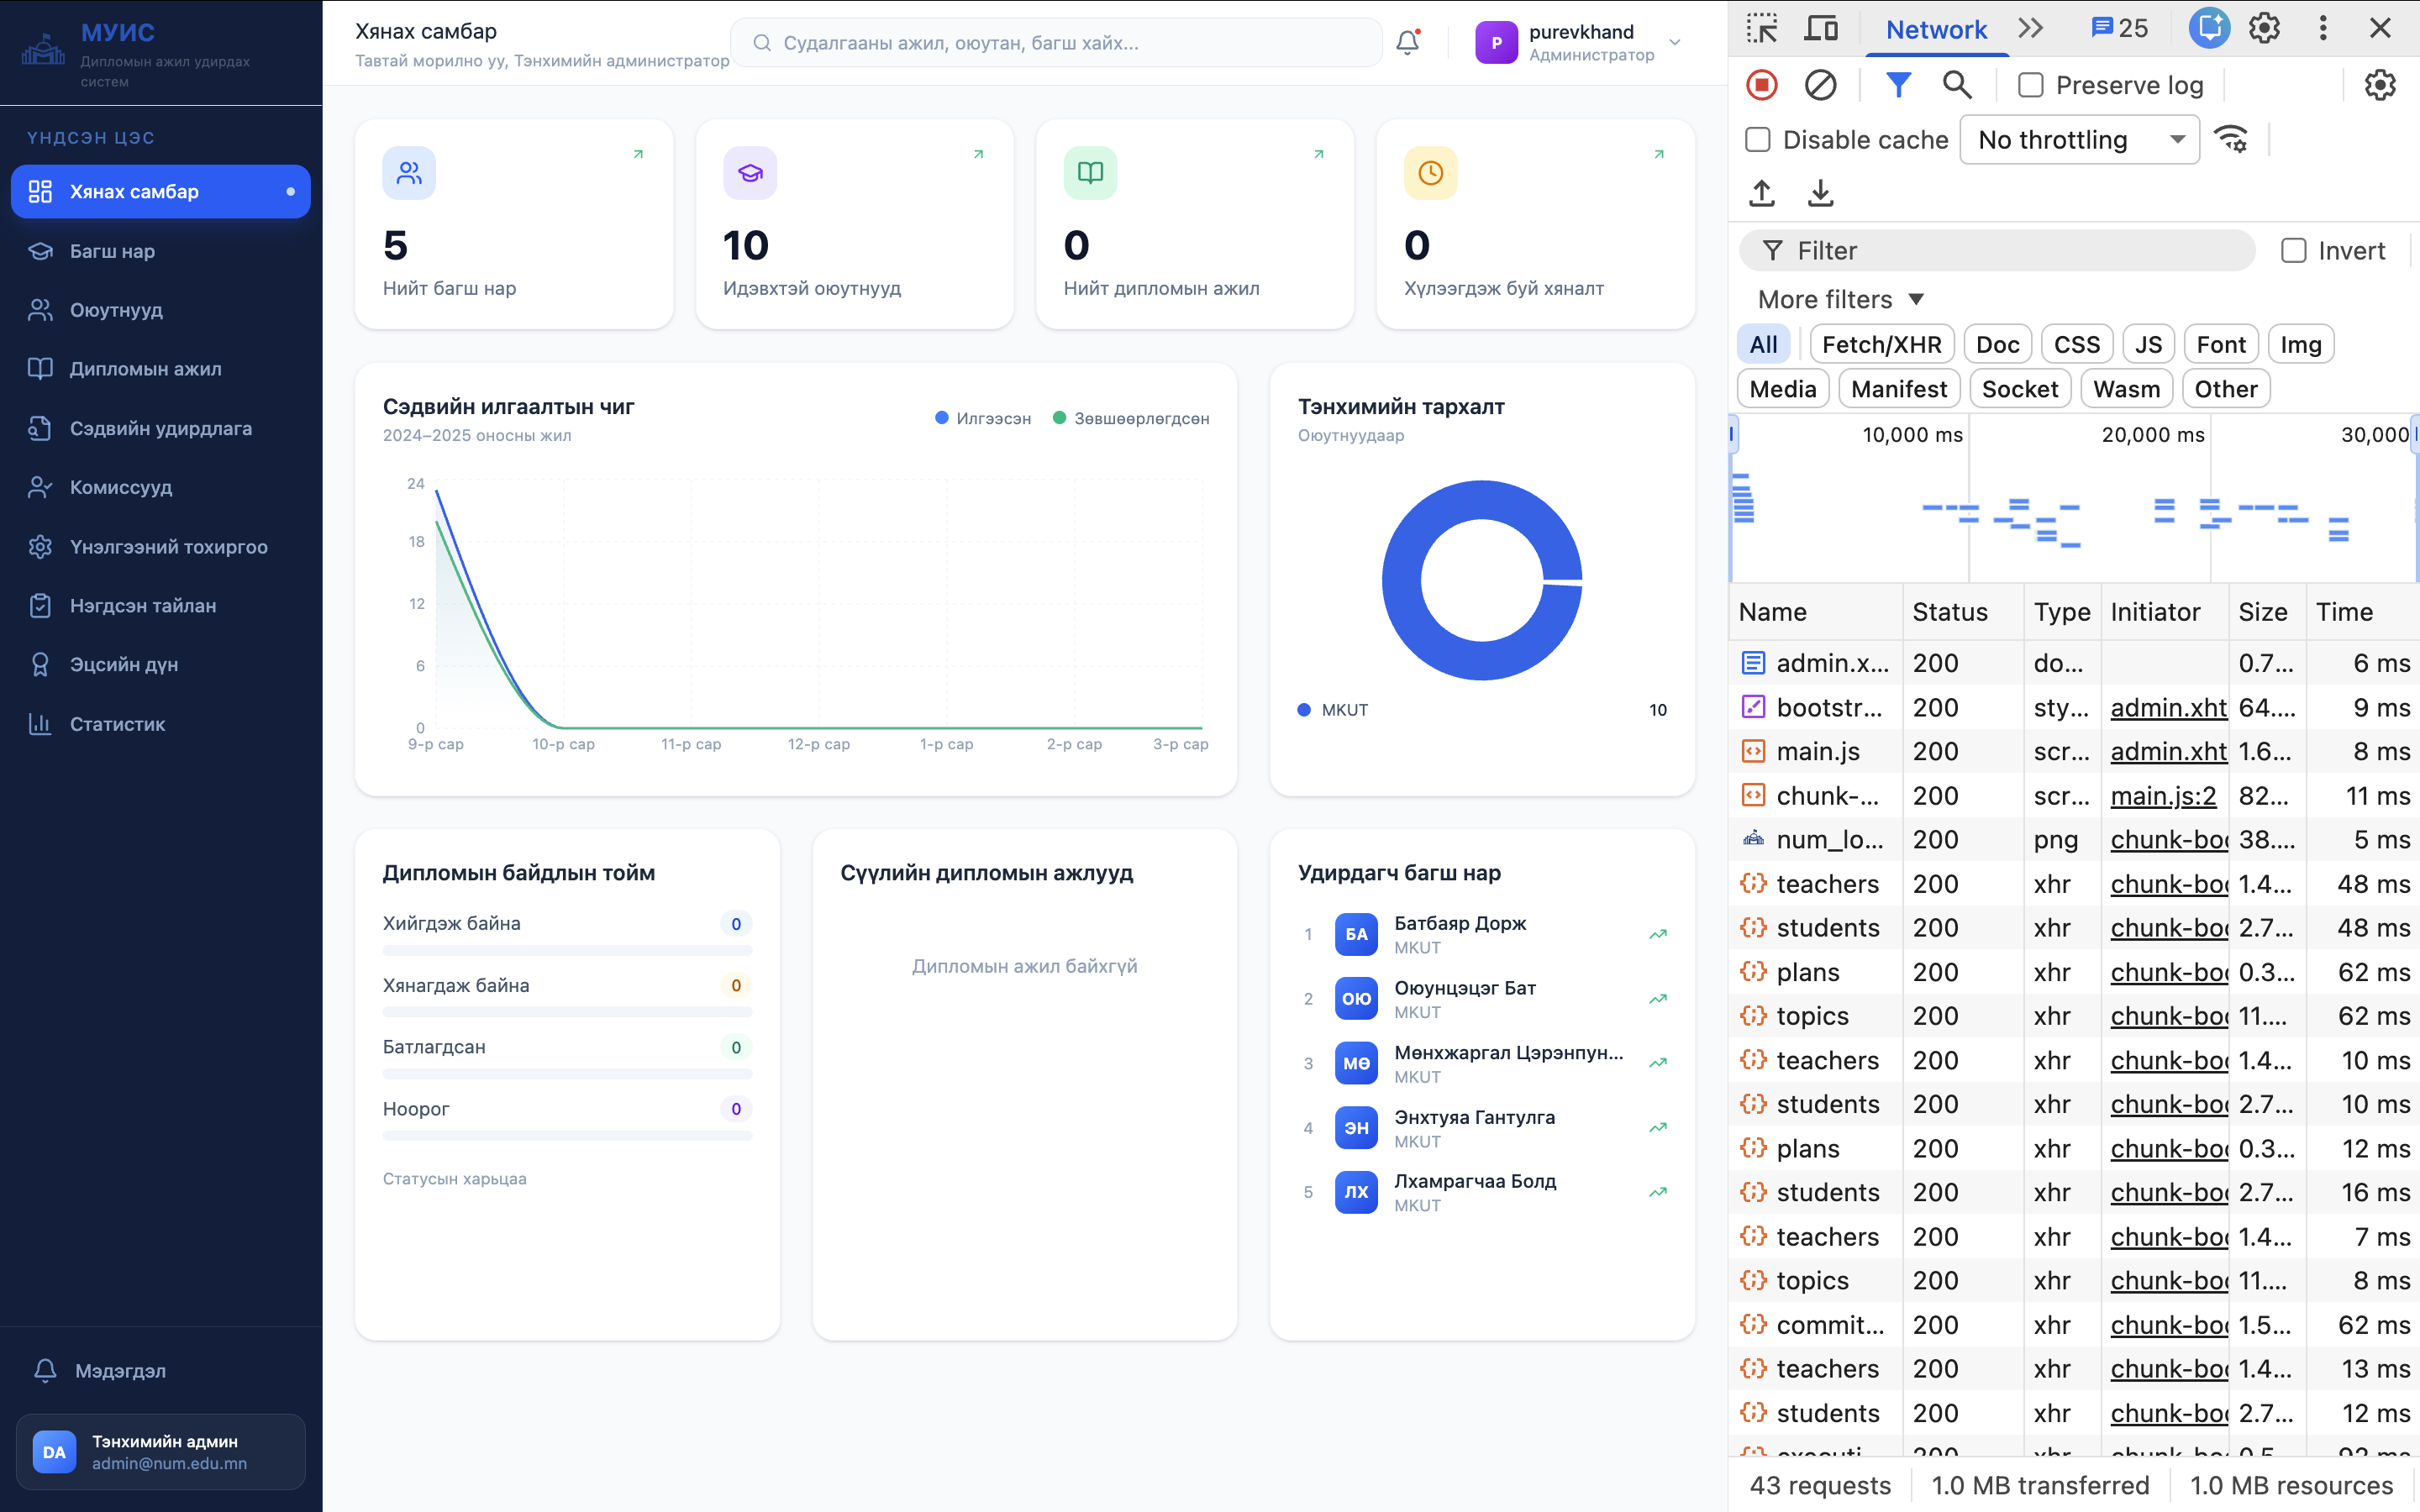
\includegraphics[width=14cm]{images/fig_implementation_summary.png}
    \caption{Зураг 4.10. Системийн хэрэгжүүлэлтийн нэгдсэн бүдүүвч. Frontend MFE давхарга, Tomcat хост, backend микросервис, PostgreSQL өгөгдлийн давхарга нь нэгдсэн байдлаар хамтарч ажилладаг бүрэн дүр зургийг харуулна. Эх сурвалж: зохиогчийн судалгаа, 2026.}
    \label{fig:impl_summary}
\end{figure}
 гэж үндсэн файлд оруулна
% Шаардлагатай package-ууд: booktabs, float, graphicx, listings,
%   tabularx, amsmath, hyperref
% =====================================================================

3-р бүлэгт тодорхойлсон архитектурын загвар нь хийсвэр зарчмуудын
цуглуулга~--- энэхүү бүлэгт эдгээр зарчмуудыг бодит кодын дэс дараа,
тохиргооны файл, алдааны дүн шинжилгээ, инженерчлэлийн практик
шийдлийн хэлбэрт хувиргасан ажлыг баримтжуулна. Загварын ``юу'' нь
хэрэгжүүлэлтийн ``хэрхэн'' болж хувирах явцад тулгарсан техникийн
хүндрэл, нарийн шийдвэр, хийсвэрлэлийн тохируулгуудыг тайлбарлана.

% ─────────────────────────────────────────────────────────────────────
\section{Frontend Хэрэгжүүлэлт ба Нэгтгэлт}
% ─────────────────────────────────────────────────────────────────────

\subsection{Vite Module Federation-ийн Тохиргоо}

3-р бүлэгт Runtime Integration стратегийг сонгосны практик хэрэгжүүлэлт нь
\texttt{@originjs/vite-plugin-federation} хэрэгсэлд тулгуурласан. Уг
хэрэгсэл нь Webpack~5-ийн \texttt{ModuleFederationPlugin}-ийн Vite орчинд
ажилладаг хувилбар бөгөөд \texttt{remoteEntry.js} файл үүсгэж, Remote
MFE-ийн экспортлосон бүрэлдэхүүнүүдийг Host-д ачаалах боломжийг хангана.

MFE модуль тус бүрийн \texttt{vite.config.ts} нь дараах бүтэцтэй тохиргоог
дагана. \texttt{module-thesis} модулийн тохиргоо нь дараах байдалтай:

\begin{figure}[H]
    \centering
    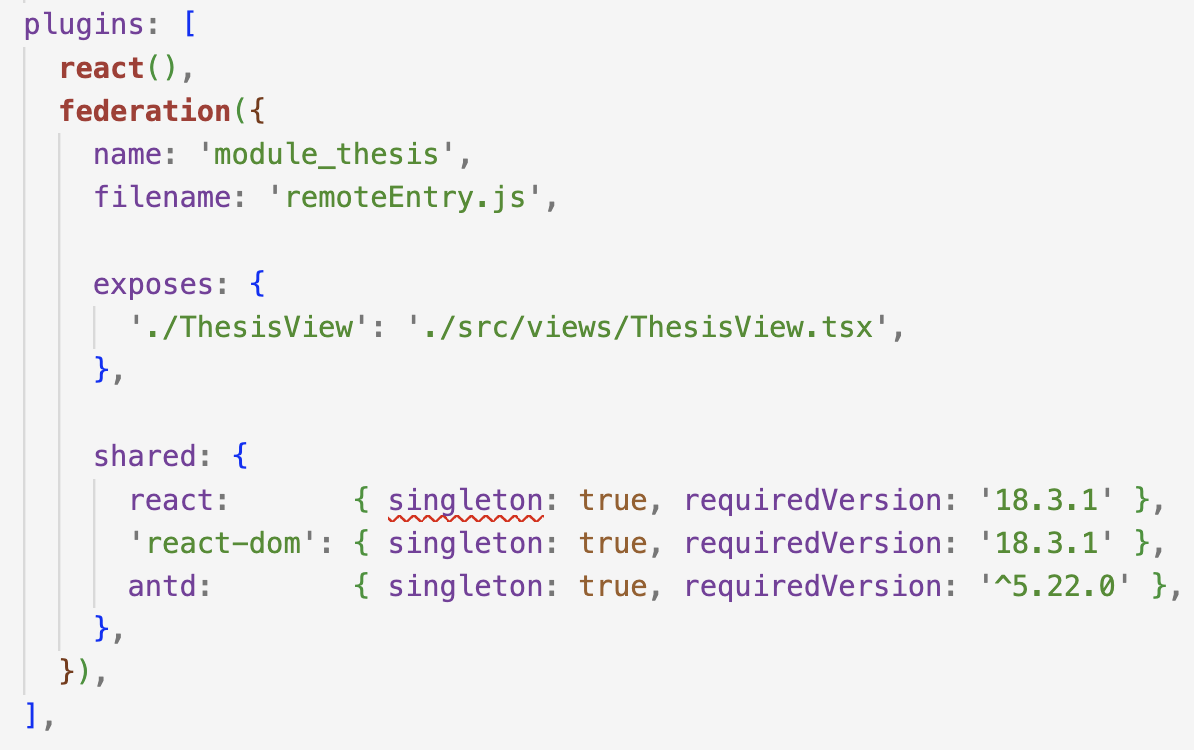
\includegraphics[width=14cm]{images/fig_vite_federation_config.png}
    \caption{Зураг 4.1. \texttt{module-thesis}-ийн \texttt{vite.config.ts} тохиргооны бүтэц. \texttt{name}, \texttt{filename}, \texttt{exposes}, \texttt{shared} дөрвөн гол тохиргооны цэгийг харуулна.}
    \label{fig:vite_config}
\end{figure}

Тохиргооны дөрвөн тулгуур параметрийг тайлбарлая:

\textbf{\texttt{name: 'module\_thesis'}:} Federation-ийн глобал нэрийн
орон зай (namespace). Browser-ийн \texttt{window} объект дээр энэ нэрийн
дор модулийн бүртгэл хийгдэнэ. Нэрийн зөрчлөөс зайлсхийхийн тулд
дор хаяж нэг давхарга нэртэй prefix ашиглах зарчмыг дагав.

\textbf{\texttt{filename: 'remoteEntry.js'}:} Remote MFE-ийн ``агуулгын
хүснэгт'' болох файлын нэр. Host нь энэ URL-г динамикаар \texttt{<script>}
tag хэлбэрт DOM-д оруулах замаар Remote-ийн бүртгэлийг ачаалдаг.

\textbf{\texttt{exposes: \{ './ThesisView': '...' \}}:} Энэ Remote-аас
Host-д нээлттэй байх бүрэлдэхүүнүүд. Дан \texttt{'./ThesisView'} экспортлосон
нь нэгдсэн зарчмыг баримтлж байна~--- нэг Remote нь нэг бизнесийн чадвар.

\textbf{\texttt{shared: \{ react, 'react-dom', antd \}}:} Singleton
хэлбэрт хуваалцагдах хамаарлууд. \texttt{singleton: true} тохиргоо нь
Host болон бүх Remote нэг React instance ашиглахыг баталгаажуулна~---
ингэснээр \texttt{useState}, \texttt{useContext} hook-ууд хөндлөн модулийн
хооронд зөв ажиллана.

\subsection{Runtime Integration: JSF-ийн Script Injection Механизм}

JSF хостын хуудсанд React MFE-г ачаалах гол механизм нь динамик
\texttt{<script>} tag injection юм. Production орчинд Tomcat~8080-д
\texttt{/microfrontends/} замаар static файлуудыг хүргэдэг бол
development орчинд \texttt{http://localhost:30XX} хаягаар Vite-ийн
dev server ажилладаг.

JSF-ийн \texttt{.xhtml} хуудсанд MFE-г ачаалах хэсэг нь дараах
ерөнхий бүтэцтэй:

\begin{figure}[H]
    \centering
    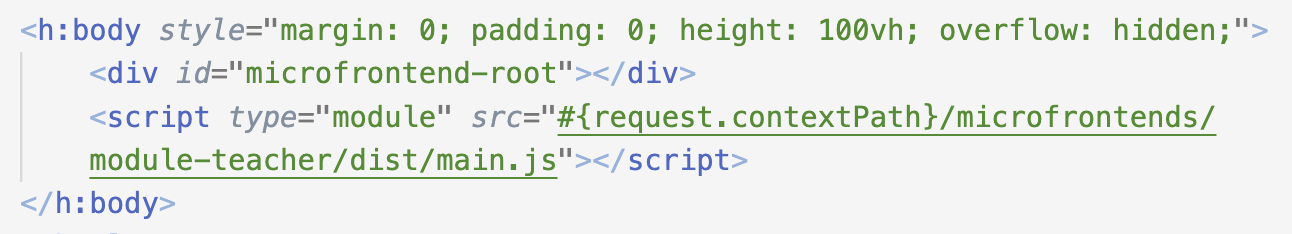
\includegraphics[width=14cm]{images/fig_jsf_script_injection.png}
    \caption{JSF \texttt{.xhtml} хуудасны MFE injection механизм. \texttt{remoteEntry.js} ачаалагдсаны дараа bootstrap.js нь \texttt{<div id="microfrontend-root">} дотор React компонентийг render хийнэ}
    \label{fig:jsf_injection}
\end{figure}

Injection-ийн техникийн дэс дараа:

\begin{enumerate}
  \item JSF Facelets нь хуудсыг server-side render хийхдээ
    \texttt{<div id="microfrontend-root"/>} DOM цэгийг байрлуулна.
  \item \texttt{<script type="module" src=".../remoteEntry.js"/>} tag
    нь браузерт Remote Federation-ийн manifest-ийг ачаална.
  \item \texttt{<script type="module">} блок нь динамик \texttt{import()}
    ашиглан Remote-ийн экспортлосон компонентийг авна.
  \item React-ийн \texttt{createRoot(\#microfrontend-root).render(\ldots)}
    нь тухайн DOM цэгт компонентийг mount хийнэ.
  \item React Router-ийн \textbf{HashRouter} ашигладгийн шалтгаан нь
    JSF-ийн FacesServlet нь \texttt{/student/*} гэх URL pattern-ийг
    хариуцдаг бөгөөд React SPA маршрутлалт нь JSF-тэй зөрчилддгийг
    арилгахын тулд \texttt{/\#/student/dashboard} хэлбэрийн hash-based
    routing хэрэглэнэ.
\end{enumerate}

\subsection{Маршрутлалтын Хүндрэл ба HashRouter Шийдэл}

MFE архитектурт маршрутлалтын хоёр давхарга байдаг: нэгдүгээр давхарга
нь JSF хостын маршрутлалт (\texttt{FacesServlet}-ийн URL pattern), хоёрдугаар
давхарга нь тухайн MFE-ийн React Router дотоод маршрутлалт. Эдгээр хоёр
давхарга зөрчилдөхөд \textbf{``404 Not Found''} буюу JSF-ийн хуудас олдохгүй
алдаа гардаг.

Энэ зөрчлийг шийдвэрлэх хоёр арга байна:

\begin{enumerate}
  \item \textbf{HistoryRouter + Server Catch-all:} Tomcat-д
    \texttt{<url-pattern>/student/*</url-pattern>} бүгдийг нэг JSF
    хуудас руу шилжүүлж, React Router-ийн \texttt{createBrowserRouter}
    ашиглана. Тохиргоо нарийн боловч хэрэглэгчийн URL чухал.
  \item \textbf{HashRouter:} URL-ийн \texttt{\#} хэсэг нь сервер рүү
    хэзээ ч явдаггүй тул JSF-тэй зөрчилддөггүй. React Router-ийн
    \texttt{HashRouter} нь \texttt{/\#/thesis/list} хэлбэрийн URL
    ашиглан дотоод маршрутлалтыг зохицуулна.
\end{enumerate}

Энэ системд \texttt{HashRouter} сонгосны шалтгаан нь: JSF-ийн \texttt{web.xml}
болон \texttt{faces-config.xml}-ийн нарийн URL pattern тохиргоог өөрчлөх
нь монолитийн дотоод урсгалд нөлөөлнө гэсэн эрсдэлтэй байсан тул
хамгийн бага өөрчлөлтийн зарчмаар \texttt{HashRouter}-ийг сонгов.

\subsection{JWT болон Глобал Төлөвийн Хуваалцалт}

JSF хост болон React MFE хоорондын хэрэглэгчийн нэвтрэлтийн мэдлэгийн
хуваалцалт нь архитектурын хамгийн нарийн хэсэг юм. Хэрэглэгч
\texttt{module-auth}-д нэвтрэхэд дараах дараалал гүйцэтгэгдэнэ:

\begin{figure}[H]
    \centering
    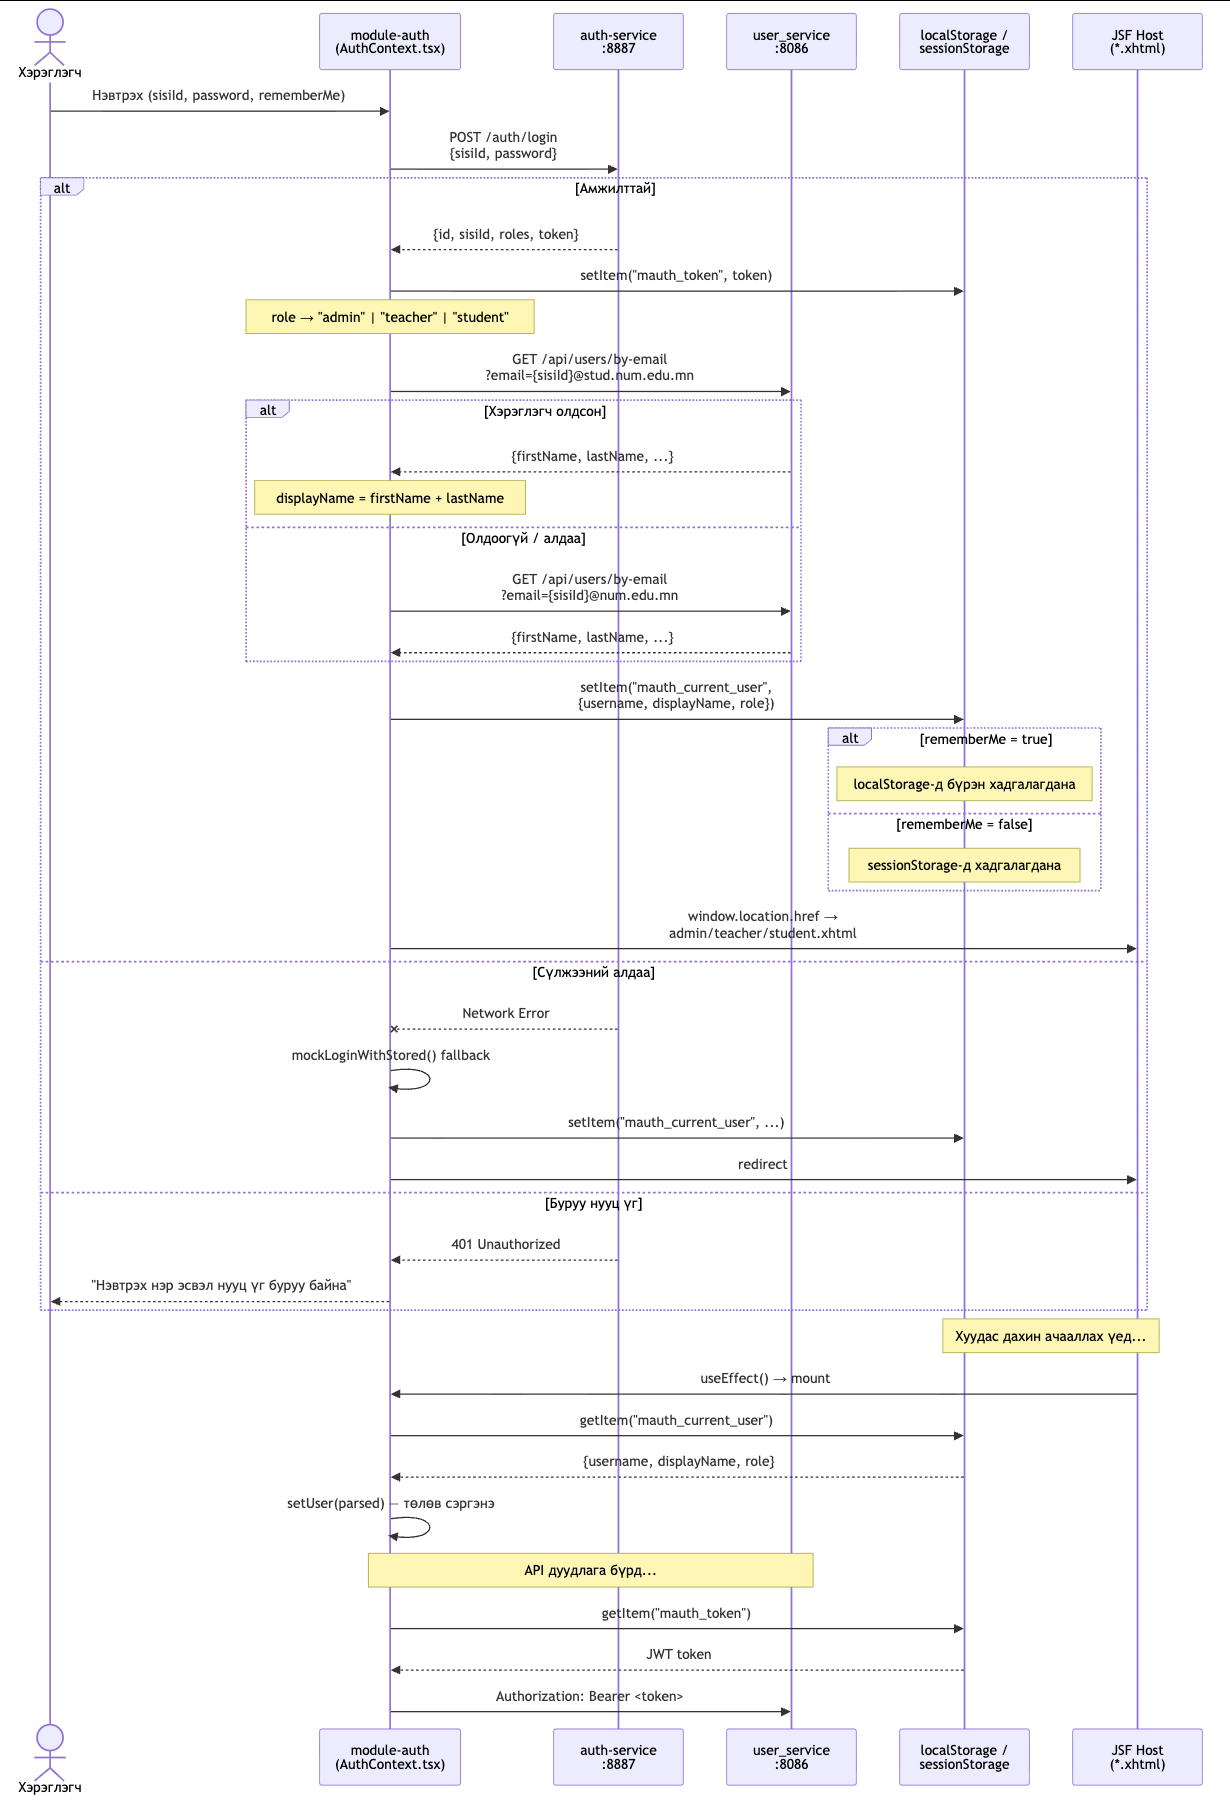
\includegraphics[width=14cm]{images/fig_jwt_flow_sequence.png}
    \caption{JWT нэвтрэлтийн дараалалт диаграм. Auth MFE нь токений хүсэлт илгээж, хүлээн авсан JWT-г localStorage-д хадгалах бөгөөд бусад MFE-ууд нь тэндээс JWT-г уншиж API дуудлагад ашиглана}
    \label{fig:jwt_flow}
\end{figure}

Хуваалцах механизм нь \texttt{localStorage} дотор тодорхой key-д JSON
объект хэлбэрт хадгалагдана:

\begin{itemize}
  \item \texttt{mauth\_token}: JWT Bearer токен~--- API дуудлага бүрийн
    \texttt{Authorization: Bearer \ldots} header-т ашиглагдана.
  \item \texttt{mauth\_current\_user}: \texttt{\{username, displayName,
    role\}} бүтэцтэй JSON~--- хэрэглэгчийн нэр, дүр зэргийг хадгалана.
\end{itemize}

Дизайн шийдвэрийн үндэслэл: \texttt{localStorage} нь хуудас дахин
ачааллагдах (page refresh) болон хэд хэдэн browser tab хооронд бүтэн
хадгалагддаг. \texttt{sessionStorage} нь tab хаагдахад устдаг тул
``Намайг санах'' (Remember Me) функцийг дэмжихгүй. Аюулгүй байдлын
хувьд \texttt{HttpOnly Cookie} нь XSS халдлагаас хамгаалалт сайн боловч
JSF-ийн хуудасны дагуу cookie scope нарийн удирдлага шаардана~---
тул энэ прототипд \texttt{localStorage} ашигласан бөгөөд үйлдвэрлэлийн
орчинд \texttt{HttpOnly} cookie руу шилжихийг зөвлөмж болгоно.

\texttt{AuthContext.tsx} нь React-ийн Context API-д суурилсан global
state provider бөгөөд MFE модуль бүрийн root-д байрладаг. Хуудас
ачааллагдах бүрт localStorage-ийн утгыг уншиж, хэрэглэгчийн төлөвийг
сэргээдэг. Нэвтрэлтийн дараалал нь дараах байна: эхлээд
\texttt{POST http://localhost:8887/auth/login} руу \texttt{\{sisiId,
password\}} илгээнэ; амжилттай тохиолдолд хариуд JWT токен болон
дүрийн мэдээлэл ирнэ; дараа нь \texttt{GET http://localhost:8086/api/users/by-email}
руу хүсэлт илгээж хэрэглэгчийн дэлгэрэнгүй нэрийг авна; эцэст нь
дүрд тохирсон URL руу чиглүүлнэ.

\subsection{Shared-UI ба Singleton Хамаарлын Зохицуулалт}

3-р бүлэгт тодорхойлсон \texttt{shared-ui} модуль нь практик хэрэгжүүлэлтэд
нарийн техникийн хүндрэлтэй тулгарав. Анх nested federation загвараар~---
\texttt{module-thesis} нь \texttt{shared\_ui} Remote-ийг агуулах~---
загварчилсан боловч хэрэгжүүлэлтийн явцад критик алдаа илэрлээ:

\texttt{TypeError: Failed to resolve module specifier '\$\{\_\_federation\_expose\_./SharedUI\}'}

Энэ алдааны үндэс нь \texttt{@originjs/vite-plugin-federation} нь
Remote-ийн \texttt{remoteEntry.js}-д Remote-ийн Remote-ийн URL template-ийг
динамикаар тохируулах механизм дутмаг байдаг явдал юм. Tomcat-д статик
файл хэлбэрт хүргэгдсэн Remote нь өөрийн nested Remote-ийн URL-г
тодорхойлж чадахгүй.

\textbf{Шийдэл:} Nested federation-ийн оронд \texttt{shared-ui}-ийн
бүрэлдэхүүнүүдийг (\texttt{PageHeader}, \texttt{PortalTabs},
\texttt{StatusBadge}, \texttt{DataTable}) тухайн Remote-ийн дотор шууд
нэгтгэж, Ant Design-ийг federation-ийн \texttt{shared singleton}
механизмаар хуваалцана. Энэ нь кодын хуулбарлалтын зардалтай боловч
runtime-д нэг antd instance ашиглагддаг тул bundle хэмжээ нэмэгдэхгүй.

\begin{figure}[H]
    \centering
    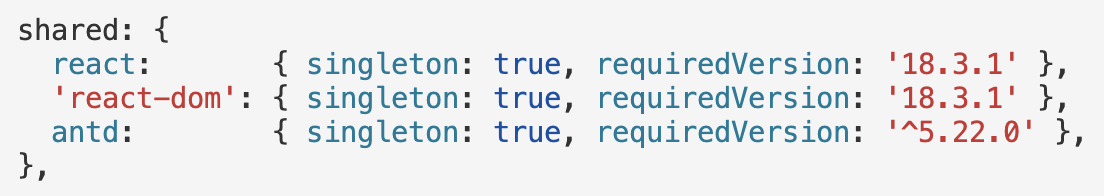
\includegraphics[width=14cm]{images/fig_shared_singleton_pattern.png}
    \caption{Shared Singleton загварын зохицуулалт. Antd нь нэгдсэн singleton хэлбэрт ачааллагдаж, Remote модуль бүр энэ нэг instance-ийг ашиглана~--- nested federation-ийн алдааг арилгана. Эх сурвалж: зохиогчийн судалгаа, 2026.}
    \label{fig:shared_singleton}
\end{figure}

\subsection{Build ба Deploy Паплайн}

Хэрэгжүүлэлтийн орчинд \texttt{build-modules.sh} shell скрипт нь
бүх MFE модулийг дараалан build хийж, \texttt{dist/} гаралтыг
Tomcat-ийн \texttt{webapps/microfrontends/\{module-name\}/dist/}
хавтаст хуулдаг. Скриптийн ерөнхий урсгал нь:

\begin{enumerate}
  \item MFE модуль бүрийн \texttt{npm run build} ажиллуулна.
  \item \texttt{dist/assets/remoteEntry.js} файлыг \texttt{dist/}
    root рүү хуулна~--- \texttt{@originjs}-ийн хуучин хувилбар нь
    \texttt{remoteEntry.js}-г \texttt{dist/assets/} дотор үүсгэдэг
    тул Host-ийн URL тохиргоотой зөрчилддгийг засна.
  \item Томкат нь \texttt{/microfrontends/\{module\}/dist/remoteEntry.js}
    замаар тухайн Remote-ийн manifest-ийг хүргэнэ.
\end{enumerate}

\begin{figure}[H]
    \centering
    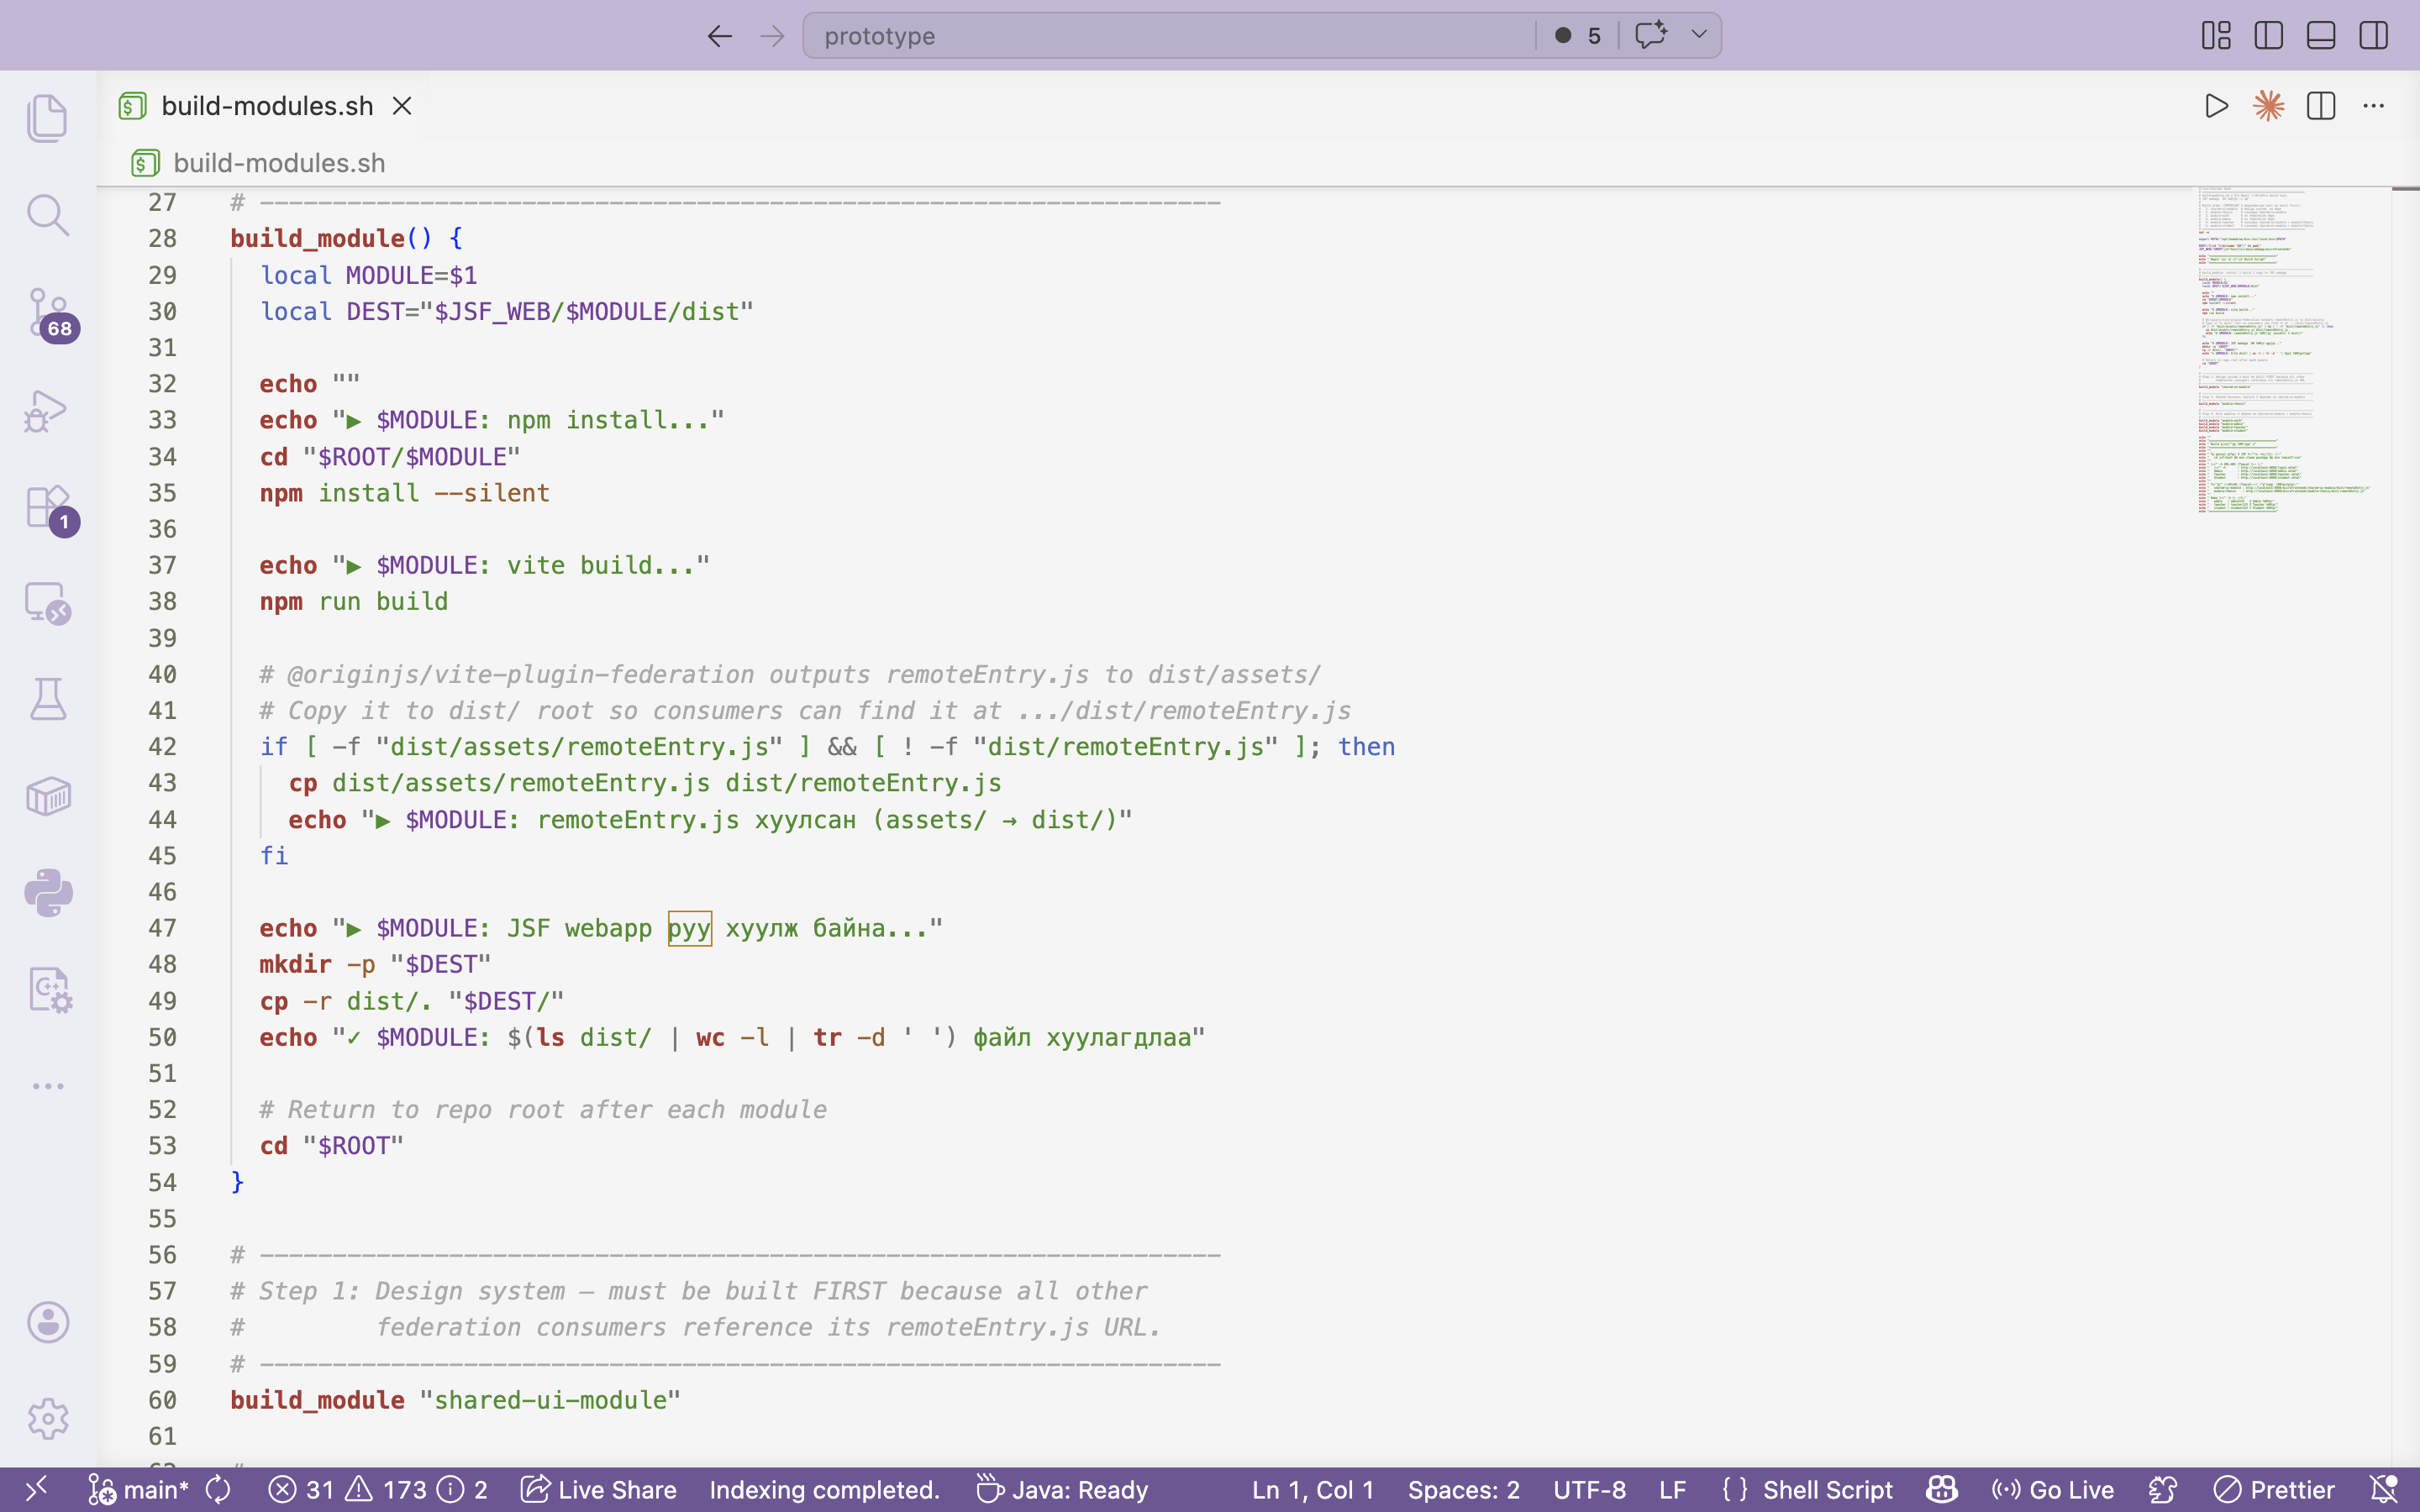
\includegraphics[width=14cm]{images/fig_build_deploy_pipeline.png}
    \caption{Зураг 4.5. Build ба Deploy паплайны урсгалын диаграм. Модуль тус бүрийн Vite build гаралт нь Tomcat-ийн webapps хавтасрт хуулагдаж, нэгдсэн байдлаар 8080 порт дээр хүргэгдэнэ. Эх сурвалж: зохиогчийн судалгаа, 2026.}
    \label{fig:build_pipeline}
\end{figure}

% ─────────────────────────────────────────────────────────────────────
\section{Backend Хэрэгжүүлэлт}
% ─────────────────────────────────────────────────────────────────────

\subsection{Spring Boot болон Spring WebFlux-ийн Сонголт}

Backend микросервисүүдийн хэрэгжүүлэлтэд Java~21 болон Spring Boot~3.2.x
framework-ийг ашиглав. Гэвч 3-р бүлгийн 3.3.2-т тодорхойлсон масштабдах
чадварын шаардлагын дагуу уламжлалт \textbf{Spring MVC} (thread-per-request)
загварын оронд \textbf{Spring WebFlux} (reactive, event-loop) загварыг
сонгов.

Spring MVC нь request бүрт нэг thread хуваарилдаг тул 1,000 зэрэгцэх
хүсэлт нь 1,000 thread шаарддаг~--- JVM-ийн thread stack дундажаар 512~КБ
тул 1,000 thread нь $\approx$~500~МБ санах ой хэрэглэнэ. Spring WebFlux
нь Netty-ийн Non-blocking I/O event-loop дээр суурилж, CPU-ийн цөмийн
тоо ($n$) thread-аар хэдэн мянган зэрэгцэх холболтыг удирддаг.

\textbf{Hexagonal Architecture (Ports and Adapters):} Сервис тус бүрийн
дотоод бүтэц нь Alistair Cockburn (2005)-ийн Hexagonal Architecture
зарчмаар зохион байгуулагдсан:

\begin{itemize}
  \item \textbf{Domain Layer:} Бизнесийн логик агуулсан цөм~---
    жишээ нь \texttt{Thesis}, \texttt{WorkflowState} домейн объектууд.
    Аль ч фреймворкоос тусгаарлагдсан цэвэр Java/Kotlin класс.
  \item \textbf{Application Layer (Ports):} Use Case интерфэйс~---
    \texttt{CreateStudentUseCase}, \texttt{FindUserUseCase},
    \texttt{SubmitThesisUseCase}. Домейн логикийг хэрхэн дуудах
    гэрээг тодорхойлно.
  \item \textbf{Adapter Layer:} Гадаад ертөнцтэй холбогч~---
    \texttt{UserController} (HTTP adapter), \texttt{UserR2dbcRepository}
    (persistence adapter), \texttt{NotificationWebSocketAdapter}
    (messaging adapter).
\end{itemize}

\begin{figure}[H]
    \centering
    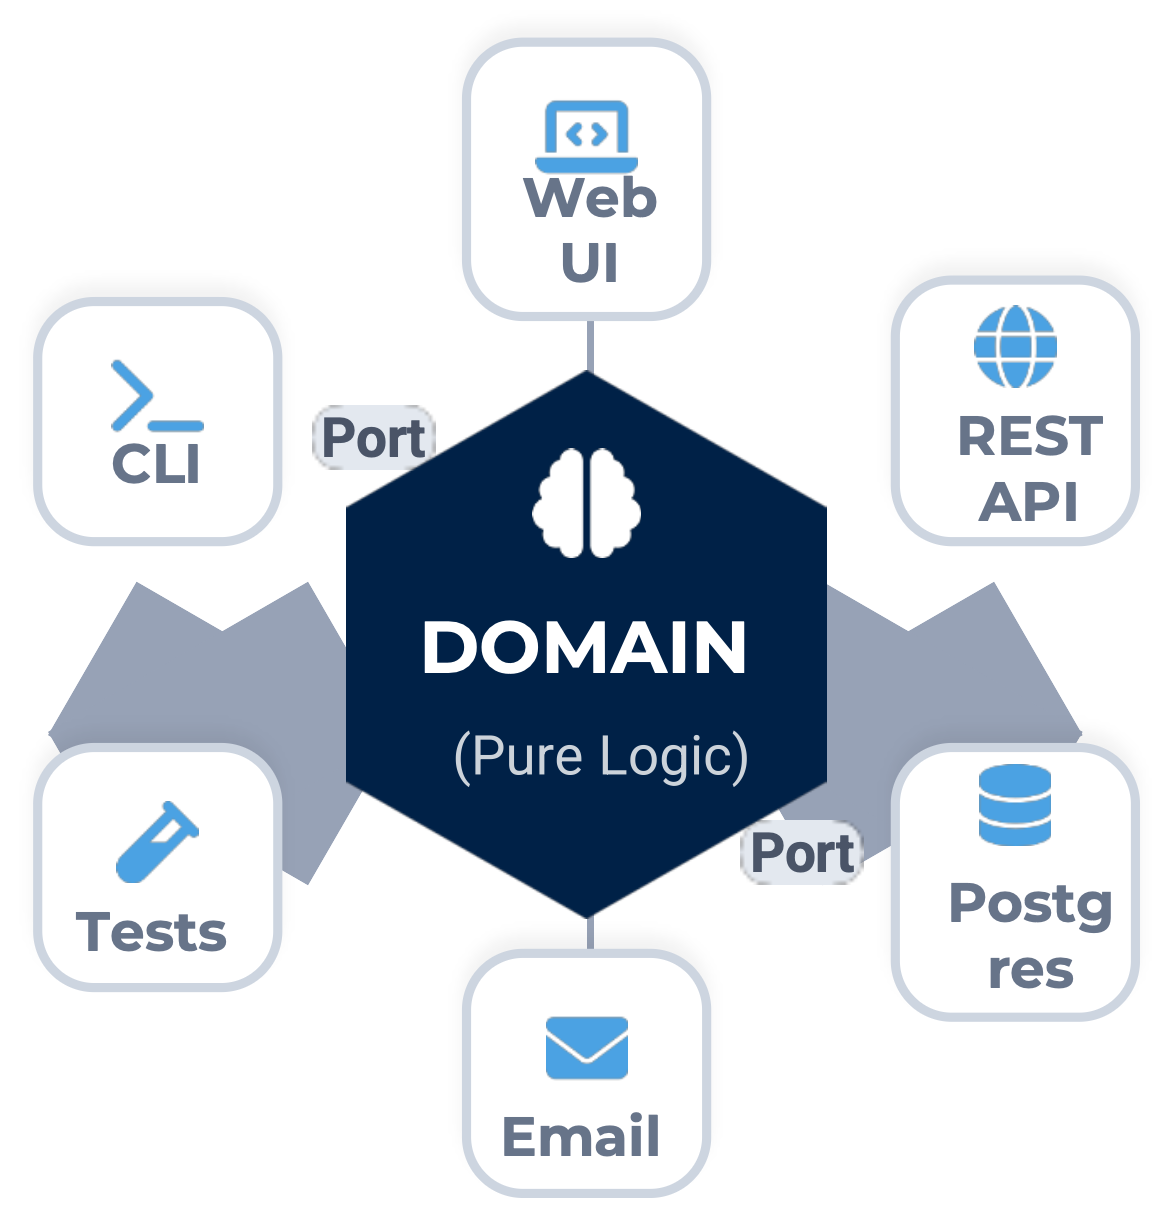
\includegraphics[width=14cm]{images/fig_hexagonal_architecture.png}
    \caption{Hexagonal Architecture-ийн \texttt{user\_service} дахь хэрэгжүүлэлтийн бүтэц. Домейн давхарга нь дотор цагирагт, Port-ууд нь дунд цагирагт, Adapter-ууд нь гадаад цагирагт байрлана. Эх сурвалж: зохиогчийн судалгаа, 2026.}
    \label{fig:hexagonal_arch}
\end{figure}

\subsection{Микросервис Тус Бүрийн Хэрэгжүүлэлтийн Нарийн}

\subsubsection{auth-service ба JWT Токений Хэрэгжүүлэлт}

\texttt{auth-service} нь \texttt{sisiId} болон нууц үг хүлээн авч, хэрэглэгчийн
бичлэгтэй харьцуулж, \texttt{jjwt}~(Java JWT) санг ашиглан токен
үүсгэнэ. Токений payload нь \texttt{\{sub: sisiId, roles: [...],
iat: epochSeconds, exp: iat+86400\}} бүтэцтэй. Нийтийн болон хувийн
түлхүүрийн хос (RSA-256)-ийн оронд энэ прототипд HMAC-SHA256 алгоритмтай
нийтлэг нууц key ашиглагдав~--- үйлдвэрлэлийн орчинд RSA key pair
болон Key Management Service (KMS) ашиглахыг зөвлөмж болгоно.

\texttt{authorization-service} нь дүр болон эрхийн матрицийг удирдана.
\texttt{ROLE\_ADMIN}, \texttt{ROLE\_TEACHER}, \texttt{ROLE\_STUDENT},
\texttt{ROLE\_COMMITTEE\_MEMBER} дүрүүд тодорхойлогдсон бөгөөд endpoint
бүр дээр Spring Security-ийн \texttt{@PreAuthorize} annotationоор
хандах эрхийн шалгалт хэрэгжинэ.

\subsubsection{user\_service-ийн Reactive Хэрэгжүүлэлт}

\texttt{user\_service} нь Spring WebFlux болон R2DBC-г хослуулан ашиглах
бөгөөд \texttt{UserController}-д хэрэглэгчийн CRUD болон хайлтын
endpoint-ууд хэрэгждэнэ. \texttt{/api/users/by-email} endpoint нь
\texttt{UserR2dbcRepository.findByEmail(String email)} reactive метод
дуудаж, \texttt{Mono<User>} буцаана~--- энэ нь AuthContext-ийн
display name lookup-д зориулан нэмэгдсэн.

\texttt{UserR2dbcRepository} нь \texttt{ReactiveCrudRepository<User, String>}
интерфэйсийг өргөтгөсөн бөгөөд Spring Data R2DBC нь SQL query-г
\texttt{findBy\{FieldName\}} нэрлэлтийн конвенцоос автоматаар үүсгэнэ.
Энэ нь ``конвенц дагасан тохиргоо'' (convention over configuration)
зарчмын практик хэрэглэлт бөгөөд boilerplate кодын хэмжээг мэдэгдэхүйц
бууруулна.

\subsubsection{workflow\_service-ийн State Machine Хэрэгжүүлэлт}

\texttt{workflow\_service} нь дипломын ажлын статус шилжилтийг хариуцна.
State Machine нь Java-ийн enum болон явцын хамгаалагдсан шилжилтийн
матрицаар хэрэгжинэ:

\begin{table}[H]
    \centering
    \caption{Дипломын ажлын статус шилжилтийн зөвшөөрөгдсөн матриц}
    \label{tab:workflow_transitions}
    \renewcommand{\arraystretch}{0.7}
    \begin{tabular}{lll}
        \toprule
        \textbf{Одоогийн статус} & \textbf{Зорилтот статус} & \textbf{Хэн гүйцэтгэх} \\
        \midrule
        DRAFT              & SUBMITTED           & Оюутан \\
        SUBMITTED          & UNDER\_REVIEW       & Удирдагч багш \\
        SUBMITTED          & REJECTED            & Удирдагч багш \\
        UNDER\_REVIEW      & REVISION\_REQUESTED & Удирдагч багш \\
        UNDER\_REVIEW      & APPROVED            & Удирдагч багш \\
        REVISION\_REQUESTED & SUBMITTED          & Оюутан \\
        APPROVED           & DEFENSE\_SCHEDULED  & Систем / Админ \\
        DEFENSE\_SCHEDULED & DEFENDED            & Хорооны гишүүн \\
        DEFENDED           & ARCHIVED            & Систем \\
        \bottomrule
    \end{tabular}
\end{table}

Зөвшөөрөгдөөгүй шилжилтийн оролдлого нь \texttt{HTTP 422 Unprocessable
Entity} буцаах бөгөөд хариу body нь шилжилт яагаад зөвшөөрөгдөхгүй
байгаа шалтгааны тайлбарыг агуулна.

\subsection{API Gateway-ийн Тохиргоо}

Тус системд тусдаа API Gateway сервис биш харин \textbf{Tomcat-ийн
reverse proxy} тохиргоо gateway-ийн үүрэг гүйцэтгэнэ. Apache Tomcat
нь \texttt{server.xml}-д \texttt{ProxyPass} директивоор (эсвэл Nginx
reverse proxy хослуулан) backend сервисүүд рүү HTTP хүсэлтийг
чиглүүлнэ. Энэ нь Nginx эсвэл Spring Cloud Gateway-тай харьцуулахад
хялбар боловч илүү нарийн CORS, rate limiting, circuit breaker
хяналт шаарддаг тул ирээдүйн шатанд тусдаа gateway нэвтрүүлэх
хэрэгцээ байна.

Frontend JavaScript-аас API дуудлагын CORS тохиргоо нь сервис
бүрийн \texttt{application.yml}-д тохируулагдсан:

\begin{figure}[H]
    \centering
    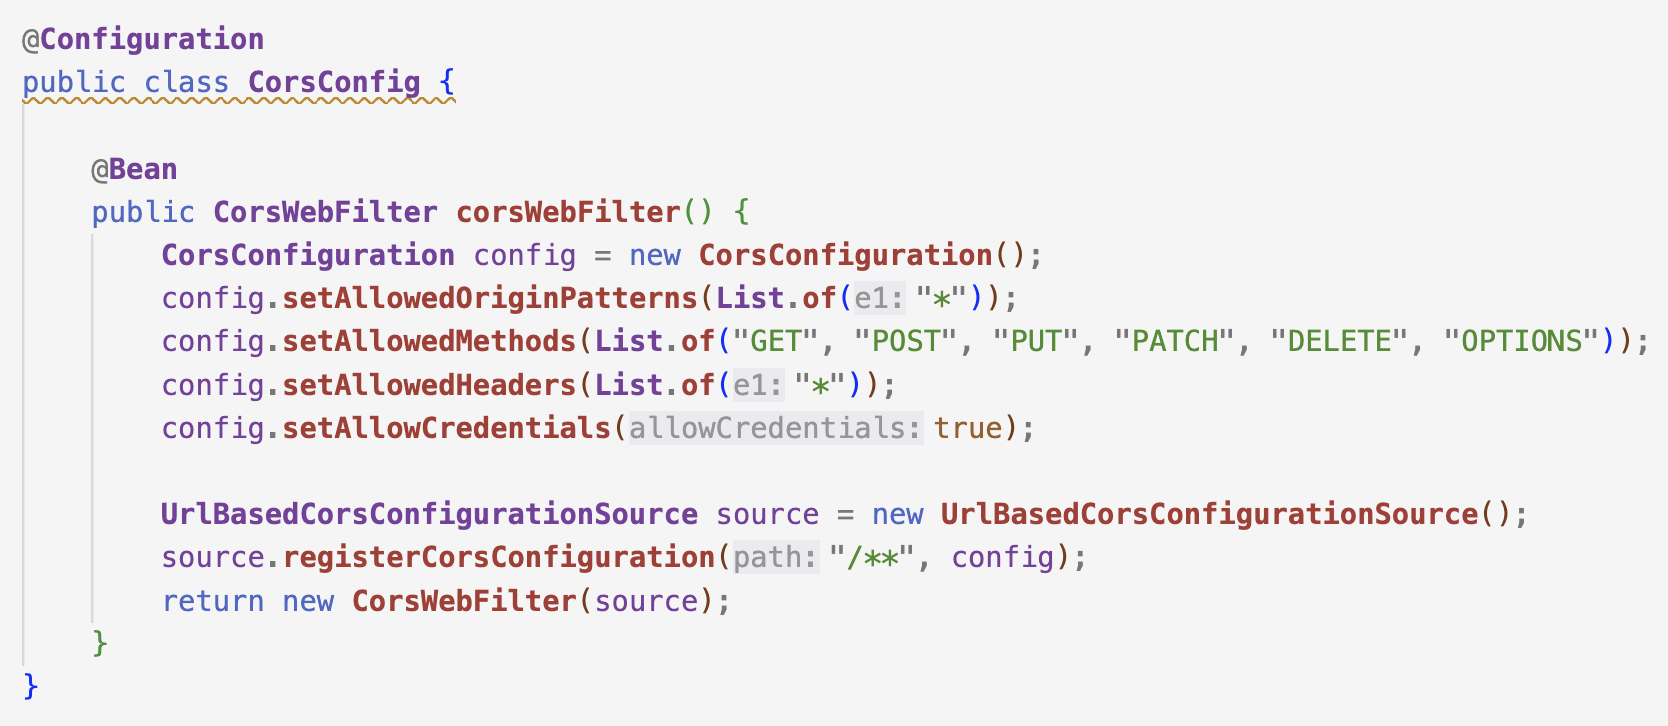
\includegraphics[width=14cm]{images/fig_cors_config.png}
    \caption{Зураг 4.7. Spring WebFlux-ийн CORS тохиргооны жишээ. \texttt{allowedOrigins} нь Tomcat-ийн 8080 порт, \texttt{allowedMethods} нь REST стандартын бүх method-уудыг агуулна. Эх сурвалж: зохиогчийн судалгаа, 2026.}
    \label{fig:cors_config}
\end{figure}

\texttt{allowedOrigins: "http://localhost:8080"} нь зөвхөн JSF хостын
хаягаас ирсэн AJAX хүсэлтийг зөвшөөрнө. Үйлдвэрлэлийн орчинд
энэ нь бодит domain нэрийг агуулна, wildcard (\texttt{*}) ашиглахаас
зайлсхийнэ.

\subsection{Distributed Tracing-ийн Хэрэгжүүлэлт}

Сервисүүдийн хоорондох хүсэлтийн урсгалыг хянах Distributed Tracing-ийг
OpenTelemetry Java Agent болон Jaeger-ийн хослолоор хэрэгжүүлэв.
JVM startup parameter-т \texttt{-javaagent:opentelemetry-agent.jar}
нэмснээр application кодыг өөрчлөхгүйгээр HTTP request бүрт
\texttt{traceparent}, \texttt{tracestate} W3C стандартын trace header
автоматаар нэмэгдэнэ.

Нэг хэрэглэгчийн хүсэлт хэд хэдэн сервисийг дамжих бүрт нэг
\texttt{traceId}-ийн дор бүх span-ууд нэгтгэгдэнэ~--- Jaeger UI-д
waterfall диаграм хэлбэрт харагддаг бөгөөд сервис бүрийн саатал
(latency contribution) тус тусад нь хэмжигдэнэ. Оюутан дипломын ажил
илгээхэд \texttt{POST /api/thesis/submit}-ийн trace нь
\texttt{auth-service} (JWT шалгах), \texttt{thesis-service}
(бичлэг шинэчлэх), \texttt{workflow-service} (статус шилжүүлэх),
\texttt{notification-service} (мэдэгдэл илгээх) гэсэн 4 span агуулдаг.

% ─────────────────────────────────────────────────────────────────────
\section{Өгөгдлийн Сангийн Хэрэгжүүлэлт}
% ─────────────────────────────────────────────────────────────────────

\subsection{PostgreSQL болон R2DBC-ийн Сонголт}

3-р бүлгийн өгөгдлийн давхаргын загварчлалд PostgreSQL-г харилцааны
(relational) өгөгдлийн санаар, R2DBC-г реактив driver хэлбэрт сонгосон
байсан. Практик хэрэгжүүлэлтэд PostgreSQL~16.2 болон
\texttt{io.r2dbc:r2dbc-postgresql:1.0.4} driver ашиглав.

\textbf{Яагаад PostgreSQL:} Дипломын ажлын бизнесийн логик нь олон
харилцаатай өгөгдлийн бүтэц (User $\leftrightarrow$ Thesis
$\leftrightarrow$ Committee $\leftrightarrow$ Evaluation) агуулдаг
тул харилцааны бүрэн бүтэн байдлын баталгаа (referential integrity),
ACID transaction, SQL-ийн хүчирхэг query боломж шаардагдана. Document
store (MongoDB) нь schema-flexible боловч JOIN-ийн хэрэгцээтэй энэ
домейнд неудобен.

\textbf{Яагаад R2DBC (JDBC биш):} Spring WebFlux-ийн event-loop
загвар нь blocking JDBC дуудлагатай ``reactive pollution'' (цуваа
блоклолт) асуудалд орно~--- blocking call нь event-loop thread-ийг
хааж, бусад хүсэлтийн хариулт удаашралд орно. R2DBC нь Non-blocking
reactive driver тул WebFlux-тэй зохистой хэрэгждэнэ.

\subsection{Schema Тодорхойлолт ба Migration}

Сервис тус бүрийн өгөгдлийн сангийн schema нь тухайн сервисийн
\texttt{src/main/resources/schema\_\{service\_name\}.sql} файлд
тодорхойлогдсон. Эхний нэвтрэлтэд Spring Boot-ийн
\texttt{spring.sql.init.mode: always} тохиргоог ашиглан schema
автоматаар үүснэ. Үйлдвэрлэлийн орчинд Flyway эсвэл Liquibase
migration хэрэгслийг ашиглахыг зөвлөмж болгоно.

\texttt{user\_service}-ийн \texttt{schema\_user\_service.sql}-ийн
гол хэсгийг жишээ болгон дурдвал:

\begin{lstlisting}[language=sql, caption={\texttt{user\_service}-ийн SQL schema-ийн жишээ. \texttt{users}, \texttt{departments} хүснэгтүүдийн DDL болон constraint-уудыг харуулна.}, label={lst:schema_sql}]
CREATE TABLE IF NOT EXISTS users (
    id              VARCHAR(255) PRIMARY KEY,
    first_name      VARCHAR(255) NOT NULL,
    last_name       VARCHAR(255) NOT NULL,
    email           VARCHAR(255) NOT NULL UNIQUE,
    department_id   VARCHAR(255),
    system_role     VARCHAR(50)  NOT NULL,
    active          BOOLEAN      NOT NULL DEFAULT TRUE,
    photo_url       VARCHAR(1000),
    created_at      TIMESTAMP    NOT NULL DEFAULT CURRENT_TIMESTAMP,
    CONSTRAINT chk_system_role
        CHECK (system_role IN ('ADMIN','STUDENT','TEACHER','DEPARTMENT_HEAD'))
);

CREATE TABLE IF NOT EXISTS students (
    id                  VARCHAR(255) PRIMARY KEY,
    user_id             VARCHAR(255) NOT NULL UNIQUE
        REFERENCES users(id) ON DELETE CASCADE,
    student_id          VARCHAR(255) NOT NULL UNIQUE,  
    major               VARCHAR(255),
    has_approved_topic  BOOLEAN NOT NULL DEFAULT FALSE
);

CREATE TABLE IF NOT EXISTS teachers (
    id                          VARCHAR(255) PRIMARY KEY,
    user_id                     VARCHAR(255) NOT NULL UNIQUE
        REFERENCES users(id) ON DELETE CASCADE,
    position                    VARCHAR(255),
    supervisor_quota            INT NOT NULL DEFAULT 5,
    current_supervised_count    INT NOT NULL DEFAULT 0,
    CONSTRAINT chk_quota_positive
        CHECK (supervisor_quota > 0),
    CONSTRAINT chk_count_non_negative
        CHECK (current_supervised_count >= 0)
);

CREATE TABLE IF NOT EXISTS departments (
    id              VARCHAR(255) PRIMARY KEY,
    user_id         VARCHAR(255) NOT NULL UNIQUE
        REFERENCES users(id) ON DELETE CASCADE,
    department_name VARCHAR(255) NOT NULL
);
CREATE INDEX IF NOT EXISTS idx_users_email       ON users(email);
CREATE INDEX IF NOT EXISTS idx_users_role        ON users(system_role);
CREATE INDEX IF NOT EXISTS idx_users_dept        ON users(department_id);
CREATE INDEX IF NOT EXISTS idx_students_user     ON students(user_id);
CREATE INDEX IF NOT EXISTS idx_students_sisi     ON students(student_id);
CREATE INDEX IF NOT EXISTS idx_teachers_user     ON teachers(user_id);
CREATE INDEX IF NOT EXISTS idx_departments_user  ON departments(user_id);

\end{lstlisting}

\texttt{user\_type} нь PostgreSQL-ийн native \texttt{ENUM} гэхийн
оронд \texttt{VARCHAR(20) CHECK (user\_type IN (...))}-ийн хэлбэрт
хэрэгжсэн~--- R2DBC-ийн хуучин хувилбарт native enum-ийн codec
авторегистр хийгддэггүй тул энэ шийдэл нь портатив, хамааралгүй.

\subsection{Connection Pooling ба Гүйцэтгэлийн Тохируулга}

R2DBC нь өөрийн \texttt{r2dbc-pool} connection pool-тай. Сервис
тус бүрийн \texttt{application.yml}-д connection pool-ийн тохиргоо
дараах байдлаар хийгдэв:

\begin{table}[H]
    \centering
    \caption{R2DBC Connection Pool-ийн тохиргооны параметрүүд}
    \label{tab:r2dbc_pool}
    \renewcommand{\arraystretch}{0.7}
    \begin{tabular}{lrl}
        \toprule
        \textbf{Параметр} & \textbf{Утга} & \textbf{Тайлбар} \\
        \midrule
        \texttt{initial-size}       & 5   & Эхлэлийн холболтын тоо \\
        \texttt{max-size}           & 20  & Хамгийн их зэрэгцэх холболт \\
        \texttt{max-idle-time}      & 30м & Идэвхгүй холболтын хамгийн их хугацаа \\
        \texttt{max-life-time}      & 60м & Холболтын нийт амьдах хугацаа \\
        \texttt{acquire-retry}      & 3   & Холболт авах оролдлогын тоо \\
        \texttt{validation-query}   & SELECT~1 & Холболт шалгах query \\
        \bottomrule
    \end{tabular}
\end{table}

\texttt{max-size: 20} нь нэг PostgreSQL-ийн default \texttt{max\_connections}
(100)-тай харьцуулахад таван сервис нэгэн зэрэг ажиллахад нийт
$5 \times 20 = 100$ холболтын хязгаарт ойрхон болно. Үйлдвэрлэлийн
орчинд \texttt{pgBouncer} connection pooler нэмэх нь PostgreSQL-ийн
connection-г дахин ашиглах боломж олгоно.

\subsection{Cross-Service Мэдээллийн Нийцэл}

Практик хэрэгжүүлэлтэд distributed transaction (2PC) ашиглахын оронд
дараах хоёр механизмыг хэрэглэв:

\textbf{Application-level Retry:} \texttt{workflow\_service}-ийн
\texttt{WebClient} нь upstream сервис рүү хүсэлт илгээхдээ
\texttt{retry(3).retryWhen(Retry.backoff(3, Duration.ofMillis(500)))}
оператораар экспоненциал backoff retry хэрэгжүүлнэ. Гурван оролдлогын
дараа амжилтгүй бол \texttt{workflow\_service} нь локал статус шилжилтийг
``rollback'' хийж, хэрэглэгчид алдааны хариу буцаана.

\textbf{Idempotency Key:} Сервисүүдийн хоорондох мутацийн хүсэлтэд
\texttt{Idempotency-Key: \{uuid\}} HTTP header ашиглана. Нэг хүсэлт
хэд хэдэн удаа хүрсэн тохиолдолд (retry эсвэл дахин дамжуулалт)
хоёр дахь хэрэгжүүлэлтийг дэд бүтэц шаардлагагүй болгоно~---
аль хэдийн хэрэгжсэн \texttt{Idempotency-Key}-тэй хүсэлтэд анхны
амжилттай хариуг буцаана.

\begin{lstlisting}[language=Java, caption={Cross-service мэдээллийн нийцлийн механизм. Retry болон Idempotency Key-ийн хослол нь eventual consistency-г хангана}, label={lst:data_consistency}]
    @PostMapping
    public Mono<ResponseEntity<DefenseSessionEntity>> create(@RequestBody CreateDefenseSessionRequest req) {
        if (!STAGE_MAX_POINTS.containsKey(req.stageType())) {
            return Mono.just(ResponseEntity.badRequest().<DefenseSessionEntity>build());
        }
        String canonicalStage = canonicalStageType(req.stageType());
        BigDecimal maxPts = req.maxPoints() != null ? req.maxPoints() : STAGE_MAX_POINTS.get(req.stageType());

        DefenseSessionEntity entity = new DefenseSessionEntity();
        entity.setId(UUID.randomUUID().toString());
        entity.setNew(true);
        entity.setDepartmentId(req.departmentId() != null ? req.departmentId() : "GLOBAL");
        entity.setCommitteeId(req.committeeId() != null ? req.committeeId() : "GLOBAL");
        entity.setStageType(canonicalStage);
        entity.setMaxPoints(maxPts);
        entity.setStatus("PENDING");
        entity.setCreatedAt(LocalDateTime.now());

        return repository.save(entity)
                .map(saved -> ResponseEntity.status(HttpStatus.CREATED).body(saved))
                .onErrorResume(org.springframework.dao.DuplicateKeyException.class, e ->
                        repository.findByCommitteeIdAndStageType(entity.getCommitteeId(), canonicalStage)
                                .map(existing -> ResponseEntity.ok(existing))
                                .defaultIfEmpty(ResponseEntity.status(HttpStatus.CONFLICT).<DefenseSessionEntity>build())
                );
    }
\end{lstlisting}

%\begin{lstlisting}[language=Java, caption={Cross-service мэдээллийн нийцлийн механизм. Retry болон Idempotency Key-ийн хослол нь eventual consistency-г хангана}, label={lst:data_consistency}]

%\end{lstlisting}

% ─────────────────────────────────────────────────────────────────────
\section{Аюулгүй Байдлын Хэрэгжүүлэлт}
% ─────────────────────────────────────────────────────────────────────

\subsection{JWT Баталгаажуулалтын Дамжуулалт}

Frontend-аас ирсэн API хүсэлт бүр \texttt{Authorization: Bearer
\{jwt\}} header агуулдаг. Backend-ийн сервис тус бүр энэ header-г
шалгана~--- auth-service руу дахин дуудлага хийхгүй, харин JWT-ийн
тоон гарын үсгийг (digital signature) орон нутагт буюу localhost-д
шалгана. Энэ нь ``token introspection'' (online validation) биш
``token verification'' (offline validation) загвар бөгөөд latency
болон auth-service-ийн ачааллыг хамгийн бага байлгана.

Spring Security-ийн \texttt{SecurityWebFilterChain} нь reactive
WebFlux контекстэд JWT filter нэмэх боломж олгодог:

\begin{enumerate}
  \item HTTP request бүрийн \texttt{Authorization} header уншина.
  \item JWT тоон гарын үсгийг нийтийн key (HMAC secret)-аар шалгана.
  \item Токений \texttt{exp} (expiration) талбарыг шалгана.
  \item Шалгалт амжилттай бол \texttt{roles} claim-ийг уншиж
    \texttt{ReactiveSecurityContextHolder}-д байрлуулна.
  \item \texttt{@PreAuthorize("hasRole('TEACHER')")} annotation нь
    энэ context-аас дүрийг шалгана.
\end{enumerate}

\subsection{CORS болон Аюулгүй байдлын Тохиргоо}

Cross-Origin Resource Sharing (CORS) нь браузерийн аюулгүй байдлын
механизм бөгөөд Frontend (8080) ба Backend сервисүүд (8081--8887)
хоорондын хүсэлтийг зохицуулна. Сервис тус бүрийн CORS тохиргоо нь
\texttt{allowedOrigins} нь зөвхөн Tomcat-ийн хаягийг агуулахаар
хязгаарлагдсан. \texttt{allowCredentials: true} тохиргоо нь wildcard
origin-тэй хамтарч ажиллахгүй тул тусгай origin тодорхойлох
шаардлагатай.

% ─────────────────────────────────────────────────────────────────────
\section{Хэрэгжүүлэлтийн Нэгтгэсэн Дүгнэлт}
% ─────────────────────────────────────────────────────────────────────

Энэхүү бүлэгт 3-р бүлгийн хийсвэр загварчлалыг практик кодын дэс
дараа болгон хэрэгжүүлсэн ажлыг баримтжуулав. Хэрэгжүүлэлтийн явцад
тулгарсан гол техникийн шийдвэрүүдийг дараах хүснэгтэд нэгтгэн
харуулав:

\begin{table}[H]
    \centering
    \caption{Загварчлалын шийдвэр ба хэрэгжүүлэлтийн шийдлийн хооронд зөрөөний бүртгэл}
    \label{tab:design_vs_impl}
    \renewcommand{\arraystretch}{0.7}
    \begin{tabular}{p{4cm}p{4.5cm}p{4.5cm}}
        \toprule
        \textbf{Асуудал} & \textbf{Загварчлалын шийдвэр} & \textbf{Хэрэгжүүлэлтийн шийдэл} \\
        \midrule
        Shared UI хуваалцалт & Nested federation & Shared singleton (antd) \\
        Маршрутлалтын зөрчил & HistoryRouter & HashRouter (\texttt{\#} prefix) \\
        remoteEntry.js байршил & dist/ root & assets/-аас root-д хуулах \\
        Хэрэглэгч мэдлэгийн хуваалцалт & SharedScope & localStorage + AuthContext \\
        API Gateway & Тусдаа сервис & Tomcat reverse proxy \\
        Distributed TX & Saga Pattern & Retry + Idempotency Key \\
        Schema тусгаарлалт & Тусдаа DB & Нэг DB, schema-level тусгаарлалт \\
        \bottomrule
    \end{tabular}
\end{table}

Хүснэгт~\ref{tab:design_vs_impl}-ийн зөрөө бүр нь гутамшгийн
шинж биш~--- Agile инженерчлэлийн ``empiricism'' (туршлагаас суралцах)
зарчмын дагуу хэрэгжүүлэлтийн явцад илэрсэн бодит хязгаарлалтад
прагматик байдлаар хариулсны үр дүн юм. 3-р бүлгийн загварчлал нь
зорилгыг тодорхойлж, энэ бүлгийн хэрэгжүүлэлт нь боломжийн хязгаарт
хамгийн ойр шийдлийг олсон. Тодорхойлогдсон зөрөөнүүд нь ирээдүйн
хөгжлийн замналын оролт болж, 6-р бүлгийн нээлттэй судалгааны асуудлуудад
цааш авч үзэгдэнэ.

\begin{figure}[H]
    \centering
    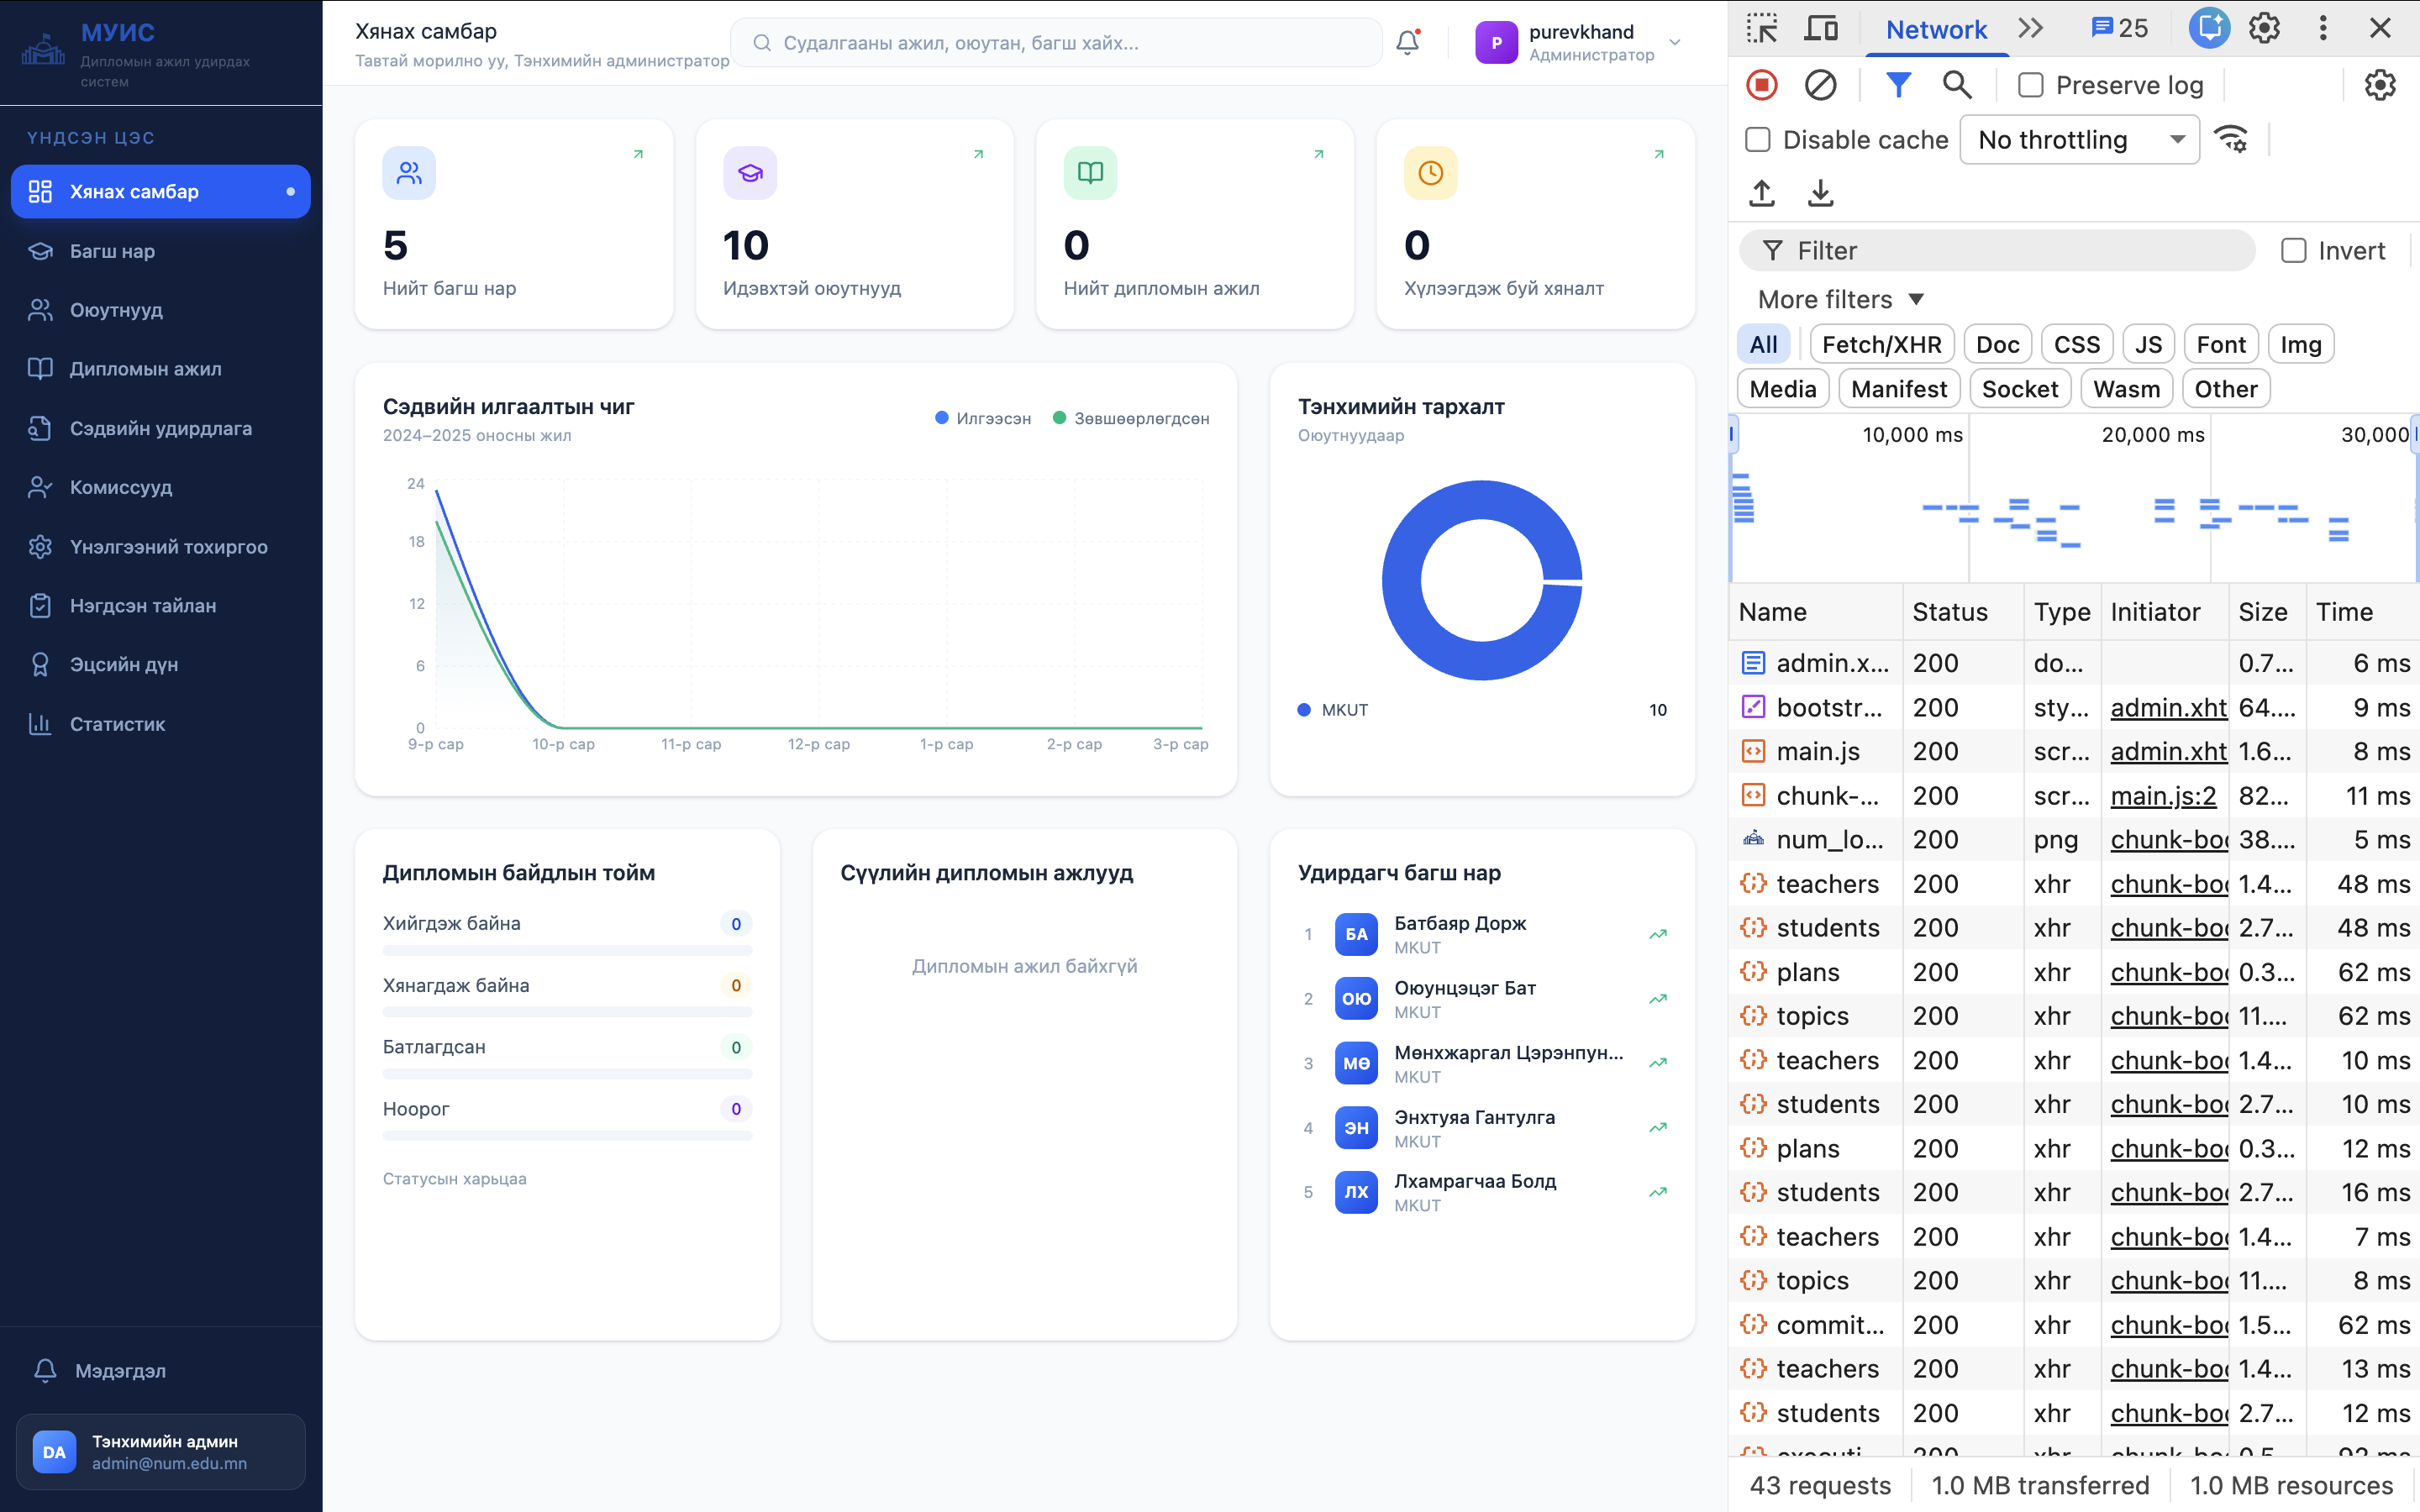
\includegraphics[width=14cm]{images/fig_implementation_summary.png}
    \caption{Зураг 4.10. Системийн хэрэгжүүлэлтийн нэгдсэн бүдүүвч. Frontend MFE давхарга, Tomcat хост, backend микросервис, PostgreSQL өгөгдлийн давхарга нь нэгдсэн байдлаар хамтарч ажилладаг бүрэн дүр зургийг харуулна. Эх сурвалж: зохиогчийн судалгаа, 2026.}
    \label{fig:impl_summary}
\end{figure}
